\section{Definition of $\seqPQ$ and Proof of Lemma \ref{lemma:EPQ rules and semantics}}
\label{sec:appendix definition of seqPQ and proof of Lemma EQP rules and semantics}

A $\textit{labelled transition system}$ ($LTS$) is a tuple $\mathcal{A}=(Q,\Sigma,\rightarrow,q_0)$, where $Q$ is a set of states, $\Sigma$ is an alphabet of transition labels, $\rightarrow\subseteq Q\times\Sigma\times Q$ is a transition relation and $q_0$ is the initial state.

Let us model priority queue as an LTS $\textit{PQ} = (Q,\Sigma,\rightarrow,q_0)$ as follows:

\begin{itemize}
\setlength{\itemsep}{0.5pt}
\item[-] Each state of $Q$ is a function from $\mathbb{P}$ into a finite sequence over $\mathbb{D}$.

\item[-] The initial state $q_0$ is a function that maps each element in $\mathbb{P}$ into $\epsilon$.

\item[-] $\Sigma = \{ \textit{put}(a,p),\textit{rm}(a),\textit{rm}(\textit{empty}) \vert a \in \mathbb{D}, p \in \mathbb{P} \}$.

\item[-] The transition relation $\rightarrow$ is defined as follows:

    \begin{itemize}
    \setlength{\itemsep}{0.5pt}
    \item[-] $q_1 \xrightarrow{\textit{put}(a,p)} q_2$, if $q_1$ maps $p$ into some finite sequence $l$, and $q_2$ is the same as $q_1$, except for $p$, where it maps $p$ into $a \cdot l$.

    \item[-] $q_1 \xrightarrow{\textit{rm}(a)} q_2$, if $q_1$ maps $p$ into $l \cdot a$ for some finite sequence $l$, and $q_2$ is the same as $q_1$, except for $p$, where it maps $p$ into $l$. We also require that for each priority $p'$ such that $p' \prec p$, $q_1$ and $q_2$ map $p'$ into $\epsilon$.

    \item[-] $q_1 \xrightarrow{\textit{rm}(\textit{empty})} q_2$, if $q_1 = q_2$, and they maps each element in $\mathbb{P}$ into $\epsilon$.
    \end{itemize}
\end{itemize}

A path of an LTS is a finite transition sequence $q_0\xrightarrow{\beta_1}q_1\overset{\beta_2}{\longrightarrow}\ldots\overset{\beta_k}{\longrightarrow}q_k$ for $k\geq 0$, where $q_0$ is the initial state of the LTS. A trace of an LTS is a finite sequence $\beta_1 \cdot \beta_2 \cdot \ldots \cdot \beta_k$, where $k \geq 0$ if there exists a path $q_0\overset{\beta_1}{\longrightarrow}q_1\overset{\beta_2}{\longrightarrow}\ldots\overset{\beta_k}{\longrightarrow}q_k$ of the LTS. Let $\seqPQ$ be the set of traces of $\textit{PQ}$. The following lemma states that $\seqPQ$ is indeed the set of sequences obtained by renaming sequences accepted by $\textit{Check-PQ-Seq}$. Given $\Gamma\in \{\mathsf{EmptyRemove}, \mathsf{Unmatched-}$ $\mathsf{MaxPriority}, \mathsf{MatchedMaxPriority}\}$, let us use $l_2 \xrightarrow{\Gamma} l_1$ to mean that when we use $\textit{Check-PQ-Seq}$ to check $l_2$, we choose the branch of $\mathsf{Has\text{-}\Gamma}$ and finally recursively call $\textit{Check-PQ-Seq}$ to check $l_1$.

\EPQRulesAndSemantics*

\begin {proof}

Let $\textit{SeqPQ}_f$ be the set of data-differentiated sequences, such that $e \in \textit{SeqPQ}_f$, if $\textit{Check-PQ-}$ $\textit{Seq}(e)=\mathsf{true}$. We need to prove that $\textit{SeqPQ}_f = \seqPQ_{\neq}$.
We prove $\textit{SeqPQ}_f \subseteq \seqPQ_{\neq}$ by induction.

\begin{itemize}
\setlength{\itemsep}{0.5pt}
\item[-] It is obvious that $\epsilon \in \seqPQ$.

\item[-] If $l_1 \in \seqPQ_{\neq}$ and $l_2 \xrightarrow{\mathsf{MatchedMaxPriority}} l_1$. Then we need to prove that $l_2 \in \seqPQ$. We know that $l_1 = u \cdot v \cdot w$, such that $\mathsf{MatchedMaxPriority\text{-}Seq}(l_2,x)$ holds and $l_2 = u \cdot \textit{put}(x,p) \cdot v \cdot \textit{rm}(x) \cdot w$.

    Assume that $u = \alpha_1 \cdot \ldots \cdot \alpha_i$, $v = \alpha_{\textit{i+1}} \cdot \ldots \cdot \alpha_j$ and $w = \alpha_{\textit{j+1}} \cdot \ldots \cdot \alpha_m$. Assume that $q_0 \xrightarrow{\alpha_1} q_1 \ldots \xrightarrow{\alpha_i} q_i \xrightarrow{\alpha_{\textit{i+1}}} q_{\textit{i+1}} \ldots  \xrightarrow{\alpha_j} q_j \xrightarrow{\alpha_{\textit{j+1}}} q_{\textit{j+1}} \ldots \xrightarrow{\alpha_m} q_m$ is the path of $l_1$ on $\textit{PQ}$. For each $i \leq k \leq j$, let $q'_k$ be the same as $q_k$, except that $q'_k$ maps $p$ into $x \cdot l_k$ and $q_k$ maps $p$ into $l_k$ for some finite sequence $l_k$.

    We already know that $q_0 \xrightarrow{\alpha_1} q_1 \ldots \xrightarrow{\alpha_i} q_i$, and it is obvious that $q_i \xrightarrow{\textit{put}(x,p)} q'_i$. Since (1) all $\textit{put}$ with priority $p$ is in $u$, and (2) in $u \cdot v$, only values with priority either incomparable, or less, or equal than $p$ is removed, we can see that it is safe to add to each $q_k$ ($1 \leq k \leq j$) with a newest $x$ with priority $p$. Or we can say, $q'_i \xrightarrow{\alpha_{\textit{i+1}}} q'_{\textit{i+1}} \ldots \xrightarrow{\alpha_j} q'_j$ are transitions of $\textit{PQ}$. Since $\textit{matched}_{\prec}(u \cdot v,p)$ holds, we can see that $q_j$ maps each priority that is smaller than $p$ into $\epsilon$ and maps $p$ into $\epsilon$, and $q'_j$ maps each priority that is smaller than $p$ into $\epsilon$ and maps $p$ into $x$. Then, we can see that $q'_j \xrightarrow{\textit{rm}(x)} q_j$. We already know that that $q_j \xrightarrow{\alpha_{\textit{j+1}}} q_{\textit{j+1}} \ldots \xrightarrow{\alpha_m} q_m$. Therefore, we can see that $l_2 = u \cdot \textit{put}(x,p) \cdot v \cdot \textit{rm}(x) \in \seqPQ$.

\item[-] If $l_1 \in \seqPQ_{\neq}$ and $l_2 \xrightarrow{\mathsf{UnmatchedMaxPriority}} l_1$. Then we need to prove that $l_2 \in \seqPQ$. We know that $l_1 = u \cdot v$, such that $\mathsf{UnmatchedMaxPriority\text{-}Seq}(l_2,x)$ holds and $l_2 = u \cdot \textit{put}(x,p) \cdot v$.

    Assume that $u = \alpha_1 \cdot \ldots \cdot \alpha_i$ and $v = \alpha_{\textit{i+1}} \cdot \ldots \cdot \alpha_m$. Assume that $q_0 \xrightarrow{\alpha_1} q_1 \ldots \xrightarrow{\alpha_i} q_i \xrightarrow{\alpha_{\textit{i+1}}} q_{\textit{i+1}} \ldots  \xrightarrow{\alpha_m} q_m$ is the path of $l_1$ on $\textit{PQ}$. For each $i \leq k \leq m$, let $q'_k$ be the same as $q_k$, except that $q'_k$ maps $p$ into $x \cdot l_k$ and $q_k$ maps $p$ into $l_k$ for some finite sequence $l_k$.

    We already know that $q_0 \xrightarrow{\alpha_1} q_1 \ldots \xrightarrow{\alpha_i} q_i$, and it is obvious that $q_i \xrightarrow{\textit{put}(x,p)} q'_i$. Since (1) all $\textit{put}$ with priority $p$ is in $u$, (2) in $u \cdot v$, only values with priority either incomparable, or less, or equal than $p$ is removed, we can see that it is safe to add to each $q_k$ ($1 \leq k \leq m$) with a newest $x$ with priority $p$. Or we can say, $q'_i \xrightarrow{\alpha_{\textit{i+1}}} q'_{\textit{i+1}} \ldots \xrightarrow{\alpha_m} q'_m$ are transitions of $\textit{PQ}$. Therefore, we can see that $l_2 = u \cdot \textit{put}(x,p) \cdot v \in \seqPQ$.

\item[-] If $l_1 \in \seqPQ_{\neq}$ and $l_2 \xrightarrow{\mathsf{EmptyRemove}} l_1$. Then we need to prove that $l_2 \in \seqPQ$. We know that $l_1 = u \cdot v$, such that $\mathsf{EmptyRemove\text{-}Seq}(l_2,o)$ holds, and $l_2 = u \cdot \textit{rm}(\textit{empty}) \cdot v$ with $o=\textit{rm}(\textit{empty})$.

    Assume that $u = \alpha_1 \cdot \ldots \cdot \alpha_i$ and $v = \alpha_{\textit{i+1}} \cdot \ldots \cdot \alpha_m$. Assume that $q_0 \xrightarrow{\alpha_1} q_1 \ldots \xrightarrow{\alpha_i} q_i \xrightarrow{\alpha_{\textit{i+1}}} q_{\textit{i+1}} \ldots  \xrightarrow{\alpha_m} q_m$ is the path of $l_1$ on $\textit{PQ}$.

    We already know that $q_0 \xrightarrow{\alpha_1} q_1 \ldots \xrightarrow{\alpha_i} q_i$. Since $\textit{matched}(u)$ holds, we can see that $q_i$ maps each element in $\mathbb{P}$ into $\epsilon$, and then $q_i \xrightarrow{\textit{rm}(\textit{empty})} q_i$. We already know that $q_i \xrightarrow{\alpha_{\textit{i+1}}} q_{\textit{i+1}} \ldots \xrightarrow{\alpha_m} q_m$. Therefore, we can see that $l_2 = u \cdot \textit{rm}(\textit{empty}) \cdot v \in \seqPQ$.
\end{itemize}

To prove that $\seqPQ_{\neq} \subseteq \textit{SeqPQ}_f$, we show that given $l_2 \in \seqPQ_{\neq}$, how to construct a sequence $l_1$, such that $l_2 \xrightarrow{\Gamma} l_1$ for some $\Gamma$, and $l_1 \in \seqPQ$. Based on this, we can decompose a sequence of $\seqPQ$ into $\epsilon$, and this process ensures that this sequence is in $\textit{SeqPQ}_f$. Note that from a $l_2$ we may construct more than one $l_1$, and this does not influence the correctness of our proof.

\begin{itemize}
\setlength{\itemsep}{0.5pt}
\item[-] If $\mathsf{Has\text{-}EmptyRemoves}(l_2)$: Assume that $l_2 = u \cdot \textit{rm}(\textit{empty}) \cdot v$. It is easy to see that $\textit{matched}(u)$ holds. Let $l_1 = u \cdot v$. It is easy to see that $l_2 \xrightarrow{\mathsf{EmptyRemove}} l_1$, and $\mathsf{UnmatchedMaxPriority\text{-}Seq}(l_2,o)$ holds for some $o=\textit{rm}(\textit{empty})$.

    Assume that $u = \alpha_1 \cdot \ldots \cdot \alpha_i$ and $v = \alpha_{\textit{i+1}} \cdot \ldots \cdot \alpha_m$. Since We already know that $q_0 \xrightarrow{\alpha_1} q_1 \ldots \xrightarrow{\alpha_i} q_i \xrightarrow{\textit{rm}(\textit{empty})} q'_i \xrightarrow{\alpha_{\textit{i+1}}} q_{\textit{i+1}} \ldots  \xrightarrow{\alpha_m} q_m$ is transitions of $\textit{PQ}$. It is easy to see that $q_i = q'_i$, and they map each element in $\mathbb{P}$ into $\epsilon$. Then we can see that $q_0 \xrightarrow{\alpha_1} q_1 \ldots \xrightarrow{\alpha_i} q_i \xrightarrow{\alpha_{\textit{i+1}}} q_{\textit{i+1}} \ldots  \xrightarrow{\alpha_m} q_m$ is transitions of $\textit{PQ}$, and $l_1 \in \seqPQ$.

\item[-] If $\mathsf{Has\text{-}UnmatchedMaxPriority}(l_2)$: Assume that $l_2 = u \cdot \textit{put}(x,p) \cdot v$, such that all $\textit{put}$ with priority $p$ of $u \cdot v$ is in $u$. Let $l_1 = u \cdot v$. According to construction of $\textit{PQ}$, we can see that $\mathsf{UnmatchedMaxPriority\text{-}Seq}(l_2,x)$ holds, and $l_2 \xrightarrow{\mathsf{UnmatchedMaxPriority}} l_1$.

    Assume that $u = \alpha_1 \cdot \ldots \cdot \alpha_i$ and $v = \alpha_{\textit{i+1}} \cdot \ldots \cdot \alpha_m$. We already know that $\textit{pa} = q_0 \xrightarrow{\alpha_1} q_1 \ldots \xrightarrow{\alpha_i} q_i \xrightarrow{\textit{put}(x,p)} q_{\textit{i+}} \xrightarrow{\alpha_{\textit{i+1}}} q_{\textit{i+1}} \ldots \xrightarrow{\alpha_m} q_m$ are transitions of $\textit{PQ}$. For each $\textit{i+1} \leq k \leq m$, let $q'_k$ be the same as $q_k$, except that $q_k$ maps $p$ into some $x \cdot l_k$ for some finite sequence $l_k$, and $q'_k$ maps $p$ into $l_k$. Since (1) all $\textit{put}$ with priority $p$ of $u \cdot v$ is in $u$ and (2) $p$ is one of maximal priority of $l_2$, it is safe to remove $x$ without influence other transitions of $\textit{pa}$. Or we can say, $q_0 \xrightarrow{\alpha_1} q_1 \ldots \xrightarrow{\alpha_i} q_i \xrightarrow{\alpha_{\textit{i+1}}} q'_{\textit{i+1}} \ldots \xrightarrow{\alpha_m} q'_m$ are transitions of $\textit{PQ}$. Therefore, $l_1 \in \seqPQ$.


\item[-] If $\mathsf{Has\text{-}MatchedMaxPriority}(l_2)$: Assume that $l_2 = u \cdot \textit{put}(x,p) \cdot v \cdot \textit{rm}(x) \cdot w$, such that all $\textit{put}$ with priority $p$ of $u \cdot v \cdot w$ is in $u$. Let $l_1 = u \cdot v \cdot w$. According to construction of $\textit{PQ}$, we can see that $\mathsf{MatchedMaxPriority\text{-}Seq}(l_2,x)$ holds, and $l_2 \xrightarrow{\mathsf{MatchedMaxPriority}} l_1$.

    Assume that $u = \alpha_1 \cdot \ldots \cdot \alpha_i$, $v = \alpha_{\textit{i+1}} \cdot \ldots \cdot \alpha_j$ and $w = \alpha_{\textit{j+1}} \cdot \ldots \cdot \alpha_m$. We already know that $q_0 \xrightarrow{\alpha_1} q_1 \ldots \xrightarrow{\alpha_i} q_i \xrightarrow{\textit{put}(x,p)} q_{\textit{i+}} \xrightarrow{\alpha_{\textit{i+1}}} q_{\textit{i+1}} \ldots \xrightarrow{\alpha_j} q_j \xrightarrow{\textit{rm}(x)} q_{\textit{j+}} \xrightarrow{\alpha_{\textit{j+1}}} q_{\textit{j+1}} \ldots \xrightarrow{\alpha_m} q_m$. For each $\textit{i+1} \leq k \leq j$, let $q'_k$ be the same as $q_k$, except that $q_k$ maps $p$ into $x \cdot l_k$ for some finite sequence $l_k$, and $q'_k$ maps $p$ into $l_k$. Since (1) $p$ is one of maximal priority in $l_2$, (2) $x$ is the newest value with priority $p$ in $l_2$, and (3) $x$ is not removed until $\textit{rm}(x)$, we know that whether we keep $x$ or remove it will not influence transitions from $q_{\textit{i+1}}$ to $q_j$. Then we can see that $q_0 \xrightarrow{\alpha_1} q_1 \ldots \xrightarrow{\alpha_i} q_i \xrightarrow{\alpha_{\textit{i+1}}} q'_{\textit{i+1}} \ldots \xrightarrow{\alpha_j} q'_j \xrightarrow{\alpha_{\textit{j+1}}} q_{\textit{j+1}} \ldots \xrightarrow{\alpha_m} q_m$ are transitions of $\textit{PQ}$. Therefore, $l_1 \in \seqPQ$.
\end{itemize}

This completes the proof of this lemma. \qed
\end {proof}






\section{Proofs in Section \ref{sec:priority queue and data-independence}}
\label{sec:appendix proofs in section priority queue and data-independence}

\EPQClosedUnderProjection*

\begin {proof}

By Lemma \ref{lemma:EPQ rules and semantics}, $\seqPQ$ is equivalent to the set of sequences obtained by renaming sequences accepted by $\textit{Check-PQ-Seq}$. It is easy to see that for the predicates of $\textit{Check-PQ-Seq}$, if a sequential execution satisfy it, then its sub-sequence also satisfy it. For example, if $\textit{matched}(u)$ holds, then $\textit{matched}(u \vert D)$ holds for each set $D$ of values. This completes the proof of this lemma. \qed
\end {proof}


\DataDifferentiatedisEnoughforPQ*

\begin {proof}

To prove the $\textit{only if}$ direction, given a data-differentiated execution $e \in \mathcal{I}_{\neq}$. By assumption, it is linearizable with respect to a sequential execution $l \in S$, and the bijection between the operations of $e$ and the operations of $l$ ensures that $l$ is differentiated and belongs to $S_{\neq}$.

To prove the $\textit{if}$ direction, given an execution $e \in \mathcal{I}$. By data independence of $\mathcal{I}$, we know that there exists $e' \in \mathcal{I}_{\neq}$ and a renaming function $r$, such that $r(e') = e$. By assumption, $e'$ is linearizable with respect to a sequential execution $l' \in S_{\neq}$. Let $l=r(l')$. By data independence of $S$ it is easy to see that $l \in S$, and it is easy to see that $e \sqsubseteq l$  using the same bijection used for $e' \sqsubseteq l'$. \qed
\end {proof}





\section{Proofs in Section \ref{sec:checking inclusion by recursive procedure}}
\label{sec:appendix in section checking lnclusion by recursive procedure}




\subsection{Definition of Step-by-Step linearizablity}
\label{sec:appendix definition of step-by-step linearizability}


We introduce the notion of step-by-step linearizability, which means that from a linearization of $e \setminus x$ that satisfy the requirements of priority queue, we can obtain a linearization of $e$ that satisfy the requirements of priority queue. Its formal definition is as follows:

%\vspace{-6pt}
\begin{definition}\label{def:step-by-step linearizability}
Given $\Gamma\in \{\mathsf{EmptyRemove}, \mathsf{UnmatchedMaxPriority}, \mathsf{MatchedMaxPriority}\}$, $\Gamma$ is step-by-step linearizability, if for each data-differentiated execution $e$ where $\Gamma\mathsf{\text{-}Conc}(e,\alpha)$ for some $\alpha$, then $e \setminus \alpha \sqsubseteq \seqPQ \Rightarrow e \sqsubseteq \seqPQ$.

$\seqPQ$ is step-by-step linearizability, if each $\Gamma$ is step-by-step linearizability.
\end{definition}

Our notion of step-by-step linearizability is inspired by the step-by-step linearizability in ~\cite{DBLP:conf/icalp/BouajjaniEEH15}.


Given a data-differentiated execution $e$, we can obtain a sequence $e'$ from $e$ by adding $\textit{put}(a,p)$ (resp., $\textit{rm}(a)$, $\textit{rm}(\textit{empty})$) between each pair of $\textit{call}(\textit{put},a,p)$ and $\textit{ret}(\textit{put},a,p)$ (resp., $\textit{call}(\textit{rm},a)$ and $\textit{ret}(\textit{rm},a)$, $\textit{call}(\textit{rm},\textit{empty})$ and $\textit{ret}(\textit{rm},\textit{empty})$). Such $e'$ is called an execution with linearization points, and we call the projection of $e'$ into $m(a,b)$ the linearization of $e$.




\subsection{Obtaining New Sequences while Ensuring that they are in $\seqPQ$}
\label{sec:obtaining new sequences while ensureing that they are in SeqPQ}


Before we prove the step-by-step linearizability of $\seqPQ$, we introduce several lemmas, which are used to ensure some sub-sequences of $\seqPQ$ still belongs to $\seqPQ$. Given a data-differentiated sequence $l$ and one of its maximal priority $p$, let $O_c(l,p)$ and $O_i(l,p)$ be the set of operations with priorities comparable with $p$ and incomparable with $p$ in $l$, respectively. Similarly we can define $D_c(l,p)$ and $D_i(l,p)$ for se of values instead of set of operations. We can see that each priority of values in $O_i(l,p)$ is either larger or incomparable with priorities of values in  $O_c(l,p)$.

The following lemma shows that if a new sequence is generated by erasing some operations in $O_c(l,p)$ while keeping the remaining $O_c(l,p)$ sub-sequences in $\seqPQ$, then this new sequence is still in $\seqPQ$. Note that this is different from projection on value.

\begin{restatable}{lemma}{EraseOcStillinEPQ}
\label{lemma:erase Oc still in EPQ}
Given a data-differentiated sequential execution $l \in \seqPQ$ and a maximal priority $p$ in $l$, where $l$ does not contain $\textit{rm}(\textit{empty})$. Let $l'$ be generated from $l$ by discarding some operations in $O_c(l,p)$, and $l' \vert_{ O_c(l,p) } \in \seqPQ$. Then, $l' \in \seqPQ$.
\end{restatable}

\begin {proof}
Let $l=o_1 \cdot \ldots \cdot o_m$, and $q_0 \xrightarrow{o_1} q_1 \ldots \xrightarrow{o_m} q_m$ be the path of $l$ in $\textit{PQ}$. Assume that $l'$ is generated from $l$ by discarding $o_{\textit{ind1}},\ldots,o_{\textit{indn}}$. Let $D$ be the set such that $D$ contains $a$, if $\textit{put}(a,\_)$ is in $o_{\textit{ind1}},\ldots,o_{\textit{indn}}$. For each $i$, let $q'_i$ be generated from $q_i$ by erasing values in $D$.

For each $q'_j$ with $j \neq \textit{ind}\_\textit{-1}$, if $o_{\textit{j+1}}$ is $\textit{put}$, then it is obvious that $q'_j \xrightarrow{o_{\textit{j+1}}} q'_{\textit{j+1}}$. Else, assume $o_{\textit{j+1}} = \textit{rm}(a)$,

\begin{itemize}
\setlength{\itemsep}{0.5pt}
\item[-] If $\textit{rm}(a) \in O_c(l,p)$: By assumption, $l' \vert_{ O_c(l,p) } \in \seqPQ$. Therefore, $a$ is in $q'_j$ and is the should-be-removed value in $O_c(l,p)$. Since each priority of values in $O_i(l,p)$ is either larger or incomparable with priorities of values in $O_c(l,p)$, we can removed $a_c$ from $q'_j$, and then $q'_j \xrightarrow{o_{\textit{j+1}}} q'_{\textit{j+1}}$.

\item[-] If $\textit{rm}(a) \in O_i(l,p)$: By assumption we know that $q_j \xrightarrow{\textit{rm}(a)} q_{\textit{j+1}}$. Since $q'_j$ contains the same $D_i(l,p)$ values as $q_j$ and $q'_j$ contains less $D_c(l,p)$ values than $q_j$, we can see that $q'_j \xrightarrow{o_{\textit{j+1}}} q'_{\textit{j+1}}$.
\end{itemize}

For each $q'_{\textit{indj-1}}$, it is easy to see that $q'_{\textit{indj-1}} = q'_{\textit{indj}}$. Therefore, we can see that $l' = o_1 \cdot \ldots o_{\textit{ind1-1}} \cdot o_{\textit{ind1+1}} \cdot \ldots \in \seqPQ$. \qed
\end {proof}


The following lemma shows that if a new sequence is generated by from some time point, erasing operations in $O_i(l,p)$, then this new sequence is still in $\seqPQ$.

\begin{restatable}{lemma}{EraseOiFromSomeTimePointStillinEPQ}
\label{lemma:erase Oi from some time point still in EPQ}
Given a data-differentiated sequential execution $l \in \seqPQ$ and a maximal priority $p$ in $l$, where $l$ does not contain $\textit{rm}(\textit{empty})$. Let $l'$ be generated from $l$ by discarding operations in $O_i(l,p)$ from some time point, then, $l' \in \seqPQ$.
\end{restatable}

\begin {proof}
Let $l=o_1 \cdot \ldots \cdot o_m$, and $q_0 \xrightarrow{o_1} q_1 \ldots \xrightarrow{o_m} q_m$ be the path of $l$ in $\textit{PQ}$. Assume that $l'$ is generated from $l$ by discarding all operations $o_i$ if (1) $o_i \in O_i(l,p)$ and (2) $i \geq k$ for a specific index $k$. Let $D$ be a set such that $a \in D$, if $\textit{put}(a,\_)$ is in $l$ and not in $l'$. For each $0 \leq i \leq m$, let $q'_i$ be generated from $q_i$ by erasing values in $D$.

Let $l'=o'_1 \cdot \ldots \cdot o'_n$, and let $f$ be a function, such that $f(i)=j$, if $o'_i = o_j$.

\begin{itemize}
\setlength{\itemsep}{0.5pt}
\item[-] We can see that $f$ maps each $0 \leq i \leq \textit{k-1}$ into $i$, and $q'_0 \xrightarrow{o_1} q'_1 \ldots \xrightarrow{o_{\textit{k-1}}} q'_{\textit{k-1}}$.

\item[-] It is easy to see that $q'_{\textit{k-1}} = q'_{f(k)-1}$, and for each $i>k$, $q'_{f(k)} = q'_{f(k+1)-1}$.

\item[-] If $o_{f(k)}$ is a $\textit{put}$ operation, then it is obvious that $q'_{f(k)-1} \xrightarrow{o_k} q'_{f(k)}$. Else, if $o_{f(k)} = \textit{rm}(a)$, we can see $a$ is in $q'_{f(k)-1}$, and since (1) $q'_{f(k)-1}$ contains the same $D_c(l,p)$ values as $q_{f(k)-1}$ and $q'_{f(k)-1}$ contains less $D_i(l,p)$ values than $q_{f(k)-1}$, and (2) each priority of values in $O_i(l,p)$ is either larger or incomparable with priorities of values in  $O_c(l,p)$, we can see that $q'_{f(k)-1} \xrightarrow{o_k} q'_{f(k)}$. Similarly we can prove the case of $o_{f(j)}$ with $j > k$.
\end{itemize}

This completes the proof of this lemma. \qed
\end {proof}

The following lemma shows that we can make $\textit{put}$ with maximal priority to happen earlier.

\begin{restatable}{lemma}{MakePutWithMaxPriorityHappenEarlier}
\label{lemma:make put with maximal priority happen earlier}
Given a data-differentiated sequential execution $l \in \seqPQ$ and a maximal priority $p$ in $l$, where $l$ does not contain $\textit{rm}(\textit{empty})$. Let $l=l_1 \cdot l_2$. Let $l_3$ be the projection of $l_2$ into $\{ \textit{put}(\_,p) \}$, and $l_4$ be the projection of $l_2$ into other operations. Then, $l'=l_1 \cdot l_3 \cdot l_4 \in \seqPQ$.
\end{restatable}

\begin {proof}
Let $l=o_1 \cdot \ldots \cdot o_m$, and $q_0 \xrightarrow{o_1} q_1 \ldots \xrightarrow{o_m} q_m$ be the path of $l$ in $\textit{PQ}$. Let $l_1 = o_1 \cdot \ldots \cdot o_n$, let $l_2 = o_{\textit{n+1}} \cdot \ldots \cdot o_m$, let $l_3 = o'_{\textit{n+1}} \cdot \ldots \cdot o'_k$, let $l_4 = o'_{\textit{k+1}} \cdot \ldots \cdot o'_m$. Let $f$ be a function, such that $f(i)=j$, if $o'_i = o_j$.

Let $q'_i$ be constructed as follows:

\begin{itemize}
\setlength{\itemsep}{0.5pt}
\item[-] For $0 \leq i \leq n$, let $q'_i = q_i$.

\item[-] For $\textit{n+1} \leq i \leq k$, let $q'_i$ be obtained from $q_n$ by adding values in $o'_{\textit{n+1}} \cdot \ldots \cdot o'_i$ with priority $p$ and in the same order.

\item[-] For $\textit{k+1} \leq i \leq m$, let $q'_i$ be obtained from $q_{f(i)}$ by adding values which are (1) with priority $p$, (2) in $o'_{\textit{n+1}} \cdot \ldots \cdot o'_i$ and not removed by $o_1 \cdot \ldots \cdot o_{f(i)}$. The order of adding them is the same as $o'_{\textit{n+1}} \cdot \ldots \cdot o'_i$.
\end{itemize}

Then, our proof proceeds as follows:

\begin{itemize}
\setlength{\itemsep}{0.5pt}
\item[-] It is obvious that $q'_0 \xrightarrow{o_1} q'_1 \ldots \xrightarrow{o_n} q'_n$ and $q'_n \xrightarrow{o_{\textit{n+1}}} q'_{\textit{n+1}} \ldots \xrightarrow{o_k} q'_k$.

\item[-] For $q'_{\textit{k+1}}$: We already know that $q_{f(k+1)-1} \xrightarrow{o_{f(k+1)}} q_{f(k+1)}$, and it is easy to see that $q_{f(k+1)-1}$ is obtained from $q_n$ by adding values in $o_{\textit{n+1}} \cdot \ldots \cdot o_{f(k+1)-1}$.

    We can see that $q'_k$ is obtained from $q_n$ by adding values in $o'_{\textit{n+1}} \cdot \ldots \cdot o'_k$, and $q'_{k+1}$ is obtained from $q_{f(k+1)}$ by adding values which are (1) with priority $p$, (2) in $o'_{\textit{n+1}} \cdot \ldots \cdot o'_i$ and not removed by $o_1 \cdot \ldots \cdot o_{f(k+1)}$.

    \begin{itemize}
    \setlength{\itemsep}{0.5pt}
    \item[-] If $o_{f(k+1)}$ is an operation of non-$p$ values, then $q'_{k+1}$ is obtained from $q_{f(k+1)}$ by adding values in $o'_{\textit{n+1}} \cdot \ldots \cdot o'_i$. Since non-$p$ priority is either smaller or incomparable with $p$, we can see that $q'_k \xrightarrow{o_{f(k+1)}} q'_{\textit{k+1}}$.

    \item[-] Otherwise, it is only possible that $o_{f(k+1)} = \textit{rm}(a)$ for some value $a$ with priority $p$. We can see that $q'_{k+1}$ is obtained from $q_{f(k+1)}$ by adding values in $o'_{\textit{n+1}} \cdot \ldots \cdot o'_k$ and then remove $a$. Since $q_{f(k+1)-1} \xrightarrow{o_{f(k+1)}} q_{f(k+1)}$, in $q_{f(k+1)-1}$( and also in $q'_k$), there is no value with priority less than $p$, and $a$ is the first-input value of priority $p$. Therefore, we can see that $q'_k \xrightarrow{o_{f(k+1)}} q'_{\textit{k+1}}$.
    \end{itemize}

\item[-] For $q'_{\textit{k+i}}$ with $i>1$: We already know that $q_{f(k+i)-1} \xrightarrow{o_{f(k+i)}} q_{f(k+i)}$, and $q_{f(k+i)-1}$ is obtained from $q_{f(k+i-1)}$ by adding values in $o_{f(k+i-1)+1} \cdot \ldots \cdot o_{f(k+i)-1}$.

    We can see that $q'_{\textit{k+i}-1}$ (resp., $q'_{\textit{k+i}}$) is obtained from $q_{f(k+i-1)}$ (resp., $q_{f(k+i)}$) by adding values which are (1) with priority $p$, (2) in $o'_{\textit{n+1}} \cdot \ldots \cdot o'_i$ and not removed by $o_1 \cdot \ldots \cdot o_{f(k+i-1)}$ (resp., $o_1 \cdot \ldots \cdot o_{f(k+i)}$).

    \begin{itemize}
    \setlength{\itemsep}{0.5pt}
    \item[-] If $o_{f(k+i)}$ is an operation of non-$p$ values, then $q'_{k+i}$ is obtained from $q_{f(k+i)}$ by adding values which are (1) with priority $p$, (2) in $o'_{\textit{n+1}} \cdot \ldots \cdot o'_i$ and not removed by $o_1 \cdot \ldots \cdot o_{f(k+i-1)}$. Since non-$p$ priority is either smaller or incomparable with $p$, we can see that $q'_{\textit{k+i-1}} \xrightarrow{o_{f(k+i)}} q'_{\textit{k+i}}$.

    \item[-] Otherwise, it is only possible that $o_{f(k+i)} = \textit{rm}(a)$ for some value $a$ with priority $p$. We can see that $q'_{k+i}$ is obtained from $q_{f(k+i)}$ by adding values in $o'_{\textit{n+1}} \cdot \ldots \cdot o'_k$ and then remove $a$. Since $q_{f(k+i)-1} \xrightarrow{o_{f(k+i)}} q_{f(k+i)}$, in $q_{f(k+i)-1}$( and also in $q'_{\textit{k+i-1}}$), there is no value with priority less than $p$, and $a$ is the first-input value of priority $p$. Therefore, we can see that $q'_{\textit{k+i-1}} \xrightarrow{o_{f(k+i)}} q'_{\textit{k+i}}$.
    \end{itemize}
\end{itemize}

This completes the proof of this lemma. \qed
\end {proof}



The following lemma shows that if a new sequence is generated by make some $O_i(l,p)$ behaviors to happen earlier, then this new sequence is still in $\seqPQ$.

\begin{restatable}{lemma}{MakeOiHappenEarlierStillinEPQ}
\label{lemma:make Oi happen earlier still in EPQ}
Given a data-differentiated sequential execution $l \in \seqPQ$ and a maximal priority $p$ in $l$, where $l$ does not contain $\textit{rm}(\textit{empty})$. Let $l \vert_{ O_i(l,p) } = l_1 \cdot l_2$, let $l' = l_1 \cdot l_3$, where $l_3$ is the projection of $l$ into non-$l_1$ operations. Then, $l' \in \seqPQ$.
\end{restatable}

\begin {proof}
Let $l=o_1 \cdot \ldots \cdot o_m$, and $q_0 \xrightarrow{o_1} q_1 \ldots \xrightarrow{o_m} q_m$ be the path of $l$ in $\textit{PQ}$. Let $l_1 = o'_1 \cdot \ldots \cdot o'_n$, let $l_3 = o'_{\textit{n+1}} \cdot \ldots \cdot o'_m$. Let $f$ be a function, such that $f(i)=j$, if $o'_i = o_j$. Let $D$ be the set of values which are added and not removed in $o'_1 \cdot \ldots \cdot o'_n$.

Let $q'_i$ be constructed as follows:

\begin{itemize}
\setlength{\itemsep}{0.5pt}
\item[-] It is easy to see that $l_1 \in \seqPQ$, and let $q'_0 \xrightarrow{o'_1} q'_1 \ldots \xrightarrow{o'_n} q'_n$ be the path of $l_1$ in $\textit{PQ}$.

\item[-] For $\textit{n+1} \leq i \leq m$, let $q'_i$ be obtained from $q_{f(i)}$ by adding values in $D$. The order of adding them is the same as $o'_1 \cdot \ldots \cdot o'_n$.
\end{itemize}

Then, our proof proceeds as follows:

\begin{itemize}
\setlength{\itemsep}{0.5pt}
\item[-] We already know that $q'_0 \xrightarrow{o'_1} q'_1 \ldots \xrightarrow{o'_n} q'_n$.

\item[-] For $q'_{\textit{n+i}}$: We already know that $q_{f(n+i)-1} \xrightarrow{o_{f(n+i)}} q_{f(n+i)}$, and it is easy to see that $q_{f(n+i)-1}$ is obtained from $q_{f(n+i-1)}$ by adding $D$-values in $o_{f(n+i-1)+1} \cdot \ldots \cdot q_{f(n+i)-1}$.

     We can see that $q'_{\textit{n+i}-1}$ (resp., $q'_{\textit{n+i}}$) is obtained from $q_{f(n+i-1)}$ (resp., $q_{f(n+i)}$) by adding remanning values in $D$.

    \begin{itemize}
    \setlength{\itemsep}{0.5pt}
    \item[-] If $o_{f(n+1)}$ is an operation of $O_c(l,p)$ values, since priority in $O_i(l,p)$ is either larger or incomparable with priority in $O_c(l,p)$, we can see that $q'_n \xrightarrow{o_{f(n+1)}} q'_{\textit{n+1}}$.

    \item[-] Otherwise, it is only possible that $o_{f(k+1)} = \textit{rm}(a)$ for some value $a$ in $O_c(l,p)$. Since $q_{f(n+i)-1} \xrightarrow{o_{f(n+i)}} q_{f(n+i)}$, in $q_{f(n+i)-1}$( and also in $q'_{\textit{n+i-1}}$), there is no value with priority less than $p$, and $a$ is the first-input value of priority $p$. Therefore, we can see that $q'_{\textit{n+i-1}} \xrightarrow{o_{f(n+i)}} q'_{\textit{n+i}}$.
    \end{itemize}
\end{itemize}

This completes the proof of this lemma. \qed
\end {proof}

The following lemma shows that if a new sequence is generated by replacing a prefix with another one which make the priority queue has same content, then this new sequence is still in $\seqPQ$.

\begin{restatable}{lemma}{ReplaceEquivalentPrefixStillinEPQ}
\label{lemma:replace equivalent prefix still in EPQ}
Given a data-differentiated sequential execution $l \in \seqPQ$. Let $l=l_1 \cdot l_2$. Given $l_3 \in \seqPQ$. Assume that the priority queue has same content after executing $l_1$ and $l_3$. Let $l' = l_3 \cdot l_2$. Then, $l' \in \seqPQ$.
\end{restatable}

\begin {proof}
Let $l=o_1 \cdot \ldots \cdot o_m$ and let $q_0 \xrightarrow{o_1} q_1 \ldots \xrightarrow{o_m} q_m$ be the path of $l$ in $\textit{PQ}$. Let $l_1 = o_1 \cdot \ldots \cdot l_k$, $l_3 = o'_1 \cdot \ldots \cdot o'_n$ and let $q_0 \xrightarrow{o'_1} q'_1 \ldots \xrightarrow{o'_n} q'_n$ be the path of $l_3$ in $\textit{PQ}$.

By assumption we know that $q_k = q'_n$. Then it is not hard to see that $q_0 \xrightarrow{o'_1} q'_1 \ldots \xrightarrow{o'_n} q'_n \xrightarrow{o_{\textit{k+1}}} q_{\textit{k+1}} \ldots \xrightarrow{o_m} q_m$ is a path in $\textit{PQ}$, and then $l' \in \seqPQ_s$. By Lemma \ref{lemma:EPQ rules and semantics}, we know that $l' \in \seqPQ$. \qed
\end {proof}




\subsection{Proving Step-by-Step Linearizability of $\seqPQ$}
\label{sec:obtaining new sequences while ensureing that they are in SeqPQ}


With the help of Lemma \ref{lemma:erase Oc still in EPQ}, Lemma \ref{lemma:erase Oi from some time point still in EPQ}, Lemma \ref{lemma:make put with maximal priority happen earlier}, Lemma \ref{lemma:make Oi happen earlier still in EPQ} and Lemma \ref{lemma:replace equivalent prefix still in EPQ}, we can now prove that $\mathsf{MatchedMaxPriority}$ is step-by-step linearizability. Here we use $\textit{call}(o)$ and $\textit{ret}(o)$ as the call and return action of operation $o$, respectively.

\begin{restatable}{lemma}{EPQ1isStepByStepLinearizability}
\label{lemma:EPQ1 is step-by-step linearizability}
For each data-differentiated execution $e$ where $\mathsf{MatchedMaxPriority}\mathsf{\text{-}Conc}(e,x)$ for some $x$, then $e \setminus x \sqsubseteq \seqPQ \Rightarrow e \sqsubseteq \seqPQ$.
\end{restatable}

\begin {proof}

By assumption we know that there exists $l$, such that $e \sqsubseteq l$ and $\mathsf{MatchedMaxPriority\text{-}Seq}(l,x)$ holds. Let $p$ be the priority of $x$, then $l=u \cdot \textit{put}(x,p) \cdot v \cdot \textit{rm}(x) \cdot w$ for some $u$, $v$ and $w$. Let $e' = e \setminus x$. By assumption there exists sequence $l'$, such that $e' \sqsubseteq l' \in \seqPQ$. Let $e_{\textit{lp}}$ be an execution with linearization points of $e$ and the linearization points is added according to $l'$. Or we can say, $e_{\textit{lp}}$ is generated from $e$ by instrumenting linearization points, and the projection of $e_{\textit{lp}}$ into operations is $l'$. Let $l'_v$ be the shortest prefix of $l'$ that contains all operation of $u \cdot v$.

Let $U$, $V$ and $W$ be the set of operations of $u$, $v$ and $w$, respectively. Let us change $O_i(l,p)$ elements in $U$, $V$ and $W$, while keep $O_c(l,p)$ elements unchanged. We proceed by a loop: In the first round of the loop, we start from the first $O_i(l,p)$-value of $l'_v$, and let it be $o_h$,

\begin{itemize}
\setlength{\itemsep}{0.5pt}
\item[-] Case $1$: If in $e_{\textit{lp}}$, the linearization point of $o_h$ is before $\textit{ret}(\textit{rm},x)$, and no $O_c(l,p)$-value in $W$ happens before $o_h$. Then, $o_h$ is in the new version of $U \cup V$.

\item[-] Case $2$: Else, if in $e_{\textit{lp}}$, the linearization point of $o_h$ is before $\textit{ret}(\textit{rm},x)$, and there exists $O_c(l,p)$-value $o_w$ in $W$, such that $o_w <_{\textit{hb}} o_h$. Then, in $l'_v$, we put $o_h$ and all $O_i(l,p)$-value whose linearization points is after the linearization point of $o_h$ into new version of $W$, and then stop the process of changing $U$, $V$ and $W$.

\item[-] Case $3$: Else, if in $e_{\textit{lp}}$, the linearization point of $o_h$ is after $\textit{ret}(\textit{rm},x)$. Then, in $l'_v$, we put $o_h$ and all $O_i(l,p)$-value whose linearization points is after the linearization point of $o_h$ into new version of $W$, and then stop the process of changing $U$, $V$ and $W$.
\end{itemize}

In the next round of the loop, we consider the second $O_i(l,p)$-value of $l'_v$, and so on. Our process proceed, until either all element in $l'_v$ are in new version of $U \cup V$, or case $2$ or case $3$ happens and this process terminates. Let $U' \cup V'$ and $W'$ be the new version of $U \cup V$ and $W$ after the process terminates, respectively. Let $O_+$ be the set of operations that are moved into $U' \cup V'$ in the process, and let $O_-$ be the set of operations that are moved into $W'$ in the process.

Let $l'_{\textit{u'v'}}$ be the projection of $l'$ into $U' \cup V'$, let $O_x$ be the set of $\textit{put}(\_,p)$ while the item is not $x$ in $h$. Let $l''_a$ be the longest prefix of $l'_{\textit{u'v'}}$, where linearization of each operation of $l''_a$ is before $\textit{ret}(\textit{put},b)$ in $e_{\textit{lp}}$. Let $l''_d$ be the projection of $l'$ into operations of $O_x$ that are not in $l''_a$. Let $l''_1 = l''_a \cdot l''_d$. Let $l''_2$ be the projection of $l'$ into operations of $l'_{\textit{u'v'}}$ that are not in $l''_1$. Let $l''_3$ be the projection of $l'$ into operations which are not in $l'_{\textit{u'v'}}$. Let $l'' = l''_1 \cdot \textit{put}(x,p) \cdot l''_2 \cdot \textit{rm}(x) \cdot l''_3$.

To prove $e \sqsubseteq l''$, we define a graph $G$ whose nodes are the operations of $h$ and there is an edge from operation $o_1$ to $o_2$, if one of the following case holds

\begin{itemize}
\setlength{\itemsep}{0.5pt}
\item[-] $o_1$ happens-before $o_2$ in h,

\item[-] the operation corresponding to $o_1$ in $l''$ is before the one corresponding to $o_2$.
\end{itemize}

Assume there is a cycle in $G$. According the the property of interval order and the fact that the order of $l''$ is total, we know that there must exists $o_1$ and $o_2$, such that $o_1$ happens-before $o_2$ in $h$, but the corresponding operations are in the opposite order in $l''$. Then, we consider all possible case of $o_1$ and $o_2$ as follows: Let $O_a$ and $O_d$ be the set of operations in $l''_a$ and $l''_d$, respectively.

\begin{itemize}
\setlength{\itemsep}{0.5pt}
\item[-] If $o_2 \in l''_1 \wedge o_1 \in l''_1$:
    \begin{itemize}
    \setlength{\itemsep}{0.5pt}
    \item[-] If $o_1,o_2 \in O_a$ or $o_1,o_2 \in O_d$: Then $l'$ contradicts with happen before relation of $h$.

    \item[-] If $o_2 \in O_a \wedge o_1 \in O_d$: Then the order of linearization points of $e_{\textit{lp}}$ contradicts with happen before relation of $h$.
    \end{itemize}

\item[-] If $o_2 \in l''_1 \wedge o_1 = \textit{put}(x,p)$:
    \begin{itemize}
    \setlength{\itemsep}{0.5pt}
    \item[-] If $o_2 \in O_a$: This is impossible, since the linearization point of operations in $O_a$ is before $\textit{ret}(\textit{put},x,p)$ in $e_{\textit{lp}}$.

    \item[-] If $o_2 \in O_d$: Then $l$ contradicts with happen before relation of $h$.
    \end{itemize}

\item[-] If $o_2 \in l''_1 \wedge o_1 \in l''_2$:
    \begin{itemize}
    \setlength{\itemsep}{0.5pt}
    \item[-] If $o_2 \in O_a$: This violates the order of linearization point in $e_{\textit{lp}}$.

    \item[-] If $o_2 \in O_d$: According to $l$, we can see that $\textit{put}(x,p)$ does not happen before any operation in $O_x$. Then we can see that the linearization point of $o_1$ is before $\textit{ret}(\textit{put},x,p)$ and $o_1 \in O_a$. This violates that $o_1 \in l''_2$.
    \end{itemize}

\item[-] If $o_2 \in l''_1 \wedge o_1 = \textit{rm}(x)$:
    \begin{itemize}
    \setlength{\itemsep}{0.5pt}
    \item[-] If $o_2 \in U \cup V$: Then $l$ contradicts with happen before relation of $h$.

    \item[-] If $o_2 \in O_+$: This is impossible, since the linearization point of operations in $O_+$ is before $\textit{ret}(\textit{rm},x)$ in $e_{\textit{lp}}$.
    \end{itemize}

\item[-] If $o_2 \in l''_1 \wedge o_1 \in l''_3$:
    \begin{itemize}
    \setlength{\itemsep}{0.5pt}
    \item[-] If $o_1 \in W \wedge o_2 \in U \cup V$: Then $l$ contradicts with happen before relation of $h$.

    \item[-] If $o_1 \in W \wedge o_2 \in O_+$:

    \begin{itemize}
    \setlength{\itemsep}{0.5pt}
    \item[-] If $o_1 \in O_i(l,p)$: Then according to the construction process of $U' \cup V'$ and $W'$, we can see that $o_1 \in O_+$ and then $o_1 \in U' \cup V'$, which contradicts that $o_1 \in l''_3$.

    \item[-] If $o_1 \in O_c(l,p)$: Then according to the construction process of $U' \cup V'$ and $W'$, we can see that $o_2 \in O_-$, which contradicts that $o_2 \in O_+$.
    \end{itemize}

    \item[-] If $o_1 \in O_- \wedge o_2 \in U \cup V$:
        \begin{itemize}
        \setlength{\itemsep}{0.5pt}
        \item[-] If the reason of $o_1 \in O_-$ is case $2$: Let $o_h$ be as in case $2$. Then there exists $O_c(l,p)$-value $o_w \in W$, and in $e_{\textit{lp}}$, $\textit{ret}(o_w)$ is before $\textit{call}(o_h)$, the linearization point of $o_h$ is before the linearization point of $o_1$, and $\textit{ret}(o_1)$ is before $\textit{call}(o_2)$. Therefore, we can see that $o_w <_{\textit{hb}} o_2$, and then $l$ contradicts with happen before relation of $h$.

        \item[-] If the reason of $o_1 \in O_-$ is case $3$: Let $o_h$ be as in case $3$. Then in $e_{\textit{lp}}$, $\textit{ret}(\textit{rm},x)$ is before the linearization point of $o_h$, the linearization point of $o_h$ is before the linearization point of $o_1$, and $\textit{ret}(o_1)$ is before $\textit{call}(o_2)$. Therefore, we can see that $\textit{rm}(x) <_{\textit{hb}} o_2$, and then $l$ contradicts with happen before relation of $h$.
        \end{itemize}
    \item[-] If $o_1 \in O_- \wedge O_2 \in O_+$: This is impossible, since in $e_{\textit{lp}}$, the linearization points of operations in $O_+$ is before the linearization points of operations in $O_-$.
    \end{itemize}

\item[-] If $o_2 = \textit{put}(x,p) \wedge o_1 \in l''_2$: This is impossible, since in $e_{\textit{lp}}$, the linearization points of operations in $l''_2$ is after $\textit{ret}(\textit{put},x,p)$.

\item[-] If $o_2 = \textit{put}(x,p) \wedge o_1 = \textit{rm}(x)$: Then $l$ contradicts with happen before relation of $h$.

\item[-] If $o_2 = \textit{put}(x,p) \wedge o_1 \in l''_3$:
    \begin{itemize}
    \setlength{\itemsep}{0.5pt}
    \item[-] If $o_1 \in W$: Then $l$ contradicts with happen before relation of $h$.

    \item[-] If $o_1 \in O_-$:
         \begin{itemize}
         \setlength{\itemsep}{0.5pt}
         \item[-] If the reason of $o_1 \in O_-$ is case $2$: Let $o_h$ be as in case $2$. Then there exists $O_c(l,p)$-value $o_w \in W$, and in $e_{\textit{lp}}$, $\textit{ret}(o_w)$ is before $\textit{call}(o_h)$, the linearization point of $o_h$ is before the linearization point of $o_1$, and $\textit{ret}(o_1)$ is before $\textit{call}(\textit{put},x,p)$. Therefore, we can see that $o_w <_{\textit{hb}} \textit{put}(x,p)$, and then $l$ contradicts with happen before relation of $h$.

         \item[-] If the reason of $o_1 \in O_-$ is case $3$: Let $o_h$ be as in case $3$. Then in $e_{\textit{lp}}$, $\textit{ret}(\textit{rm},x)$ is before the linearization point of $o_h$, the linearization point of $o_h$ is before the linearization point of $o_1$, and $\textit{ret}(o_1)$ is before $\textit{call}(\textit{put},x,p)$. Therefore, we can see that $\textit{rm}(x) <_{\textit{hb}} \textit{put}(x,p)$, and then $l$ contradicts with happen before relation of $h$.
         \end{itemize}
    \end{itemize}

\item[-] If $o_2 \in l''_2 \wedge o_1 \in l''_2$: Then $l'$ contradicts with happen before relation of $h$.

\item[-] If $o_2 \in l''_2 \wedge o_1 = \textit{rm}(x)$: We can prove this similarly as the case of $o_2 \in l''_1 \wedge o_1 = \textit{rm}(x)$.

\item[-] If $o_2 \in l''_2 \wedge o_1 \in l''_3$: We can prove this similarly as the case of $o_2 \in l''_1 \wedge o_1 \in l''_3$.

\item[-] If $o_2 = \textit{rm}(x) \wedge o_1 \in l''_3$:
    \begin{itemize}
    \setlength{\itemsep}{0.5pt}
    \item[-] If $o_1 \in W$: Then $l$ contradicts with happen before relation of $h$.

    \item[-] If $o_1 \in O_-$:
         \begin{itemize}
         \setlength{\itemsep}{0.5pt}
         \item[-] If the reason of $o_1 \in O_-$ is case $2$: Let $o_h$ be as in case $2$. Then there exists $O_c(l,p)$-value $o_w \in W$, and in $e_{\textit{lp}}$, $\textit{ret}(o_w)$ is before $\textit{call}(o_h)$, the linearization point of $o_h$ is before the linearization point of $o_1$.

             Since $l$ is consistent with the happen before order of $h$, we can see that $\textit{call}(\textit{rm},x)$ is before $\textit{ret}(o_w)$. Therefore, we can see that the linearization point of $o_1$ is after $\textit{call}(\textit{rm},x)$, and then it is impossible that $o_1 <_{\textit{hb}} \textit{rm}(x)$.

         \item[-] If the reason of $o_1 \in O_-$ is case $3$: Let $o_h$ be as in case $3$. Then in $e_{\textit{lp}}$, $\textit{ret}(\textit{rm},x)$ is before the linearization point of $o_h$, and the linearization point of $o_h$ is before the linearization point of $o_1$. Therefore, we can see that the linearization point of $o_1$ is after $\textit{ret}(\textit{rm},x)$, and then it is impossible that $o_1 <_{\textit{hb}} \textit{rm}(x)$.
         \end{itemize}
    \end{itemize}

\item[-] If $o_2 \in l''_3 \wedge o_1 \in l''_3$: Then $l'$ contradicts with happen before relation of $h$.
\end{itemize}

Therefore, we know that $G$ is acyclic, and then we know that $h \sqsubseteq l''$.

It remains to prove that $l'' \in \seqPQ$. The process for proving $l'' \in \seqPQ$ is as follows:

\begin{itemize}
\setlength{\itemsep}{0.5pt}
\item[-] Since $l' \in \seqPQ$ and $l'_v$ is a prefix of $l'$, it is obvious that $l'_v \in \seqPQ$.

\item[-] $l'_{\textit{u'v'}}$ can be obtained from $l'_v$ as follows:
    \begin{itemize}
    \setlength{\itemsep}{0.5pt}
    \item[-] Discard $O_c(l,p)$-value that are in $W$ and keep $O_c(l,p)$-value in $U \cup V$ unchanged.

    \item[-] From some time point, discard all the $O_i(l,p)$ operations after this time point.
    \end{itemize}

From $\textit{matched}_{\prec}(u \cdot v,p)$, we can see that $O_c(l,p)$-value in $U \cdot V$ is matched, and then it is easy to see that the projection of $l'_v$ in to $O_c(l,p)$-value in $U \cdot V$ is still in $\seqPQ$. By Lemma \ref{lemma:erase Oc still in EPQ} and Lemma \ref{lemma:erase Oi from some time point still in EPQ}, we can see that $l'_{\textit{u'v'}} \in \seqPQ$.

\item[-] $l''_1 \cdot l''_2$ can be obtained from $l'_{\textit{u'v'}}$ as follows: Execute until reaching some time point $t$, then first execute all $O_x$ operations after $t$, and then execute remanning operations. By Lemma \ref{lemma:make put with maximal priority happen earlier}, we can see that $l''_1 \cdot l''_2 \in \seqPQ$.

\item[-] Let $l'_e$ be obtained from $l'$ by discarding $O_c(l,p)$-value in $U \cdot V$. By Lemma \ref{lem:closure_proj}, we can see that $l'_e \in \seqPQ$.

\item[-] Let $l'_e \vert_{O_i(l,p)}  = l'_f \cdot l'_g$, where $l'_f$ is the projection of $O_i(l,p)$-value in $U \cdot V$. Let $l'_h$ be obtained from $l'_e$ by discarding operations in $l'_f$. By Lemma \ref{lemma:make Oi happen earlier still in EPQ}, we can see that $l'_f \cdot l'_h \in \seqPQ$.


\item[-] By Lemma \ref{lem:closure_proj}, it is obvious that $l'_f \in \seqPQ$. From $\textit{matched}_{\prec}(u \cdot v,p)$, we can see that the content of priority queue after executing $l''_1 \cdot l''_2$ is the same as after executing $l'_f$. By Lemma \ref{lemma:replace equivalent prefix still in EPQ}, we can see that $l''_1 \cdot l''_2 \cdot l'_h \in \seqPQ$. It is easy to see that $l'_h = l''_3$, and then $l''_1 \cdot l''_2 \cdot l''_3 \in \seqPQ$.

\item[-] Since $\mathsf{MatchedMaxPriority\text{-}Seq}(l,x)$ holds, it is easy to see that $l'' = l''_1 \cdot \textit{put}(x,p) \cdot l''_2 \cdot \textit{rm}(x) \cdot l''_3 \in \seqPQ$.
\end{itemize}

Therefore, we prove that $e \sqsubseteq l'' \in \seqPQ$. This completes the proof of this lemma. \qed
\end {proof}


\begin{restatable}{lemma}{EPQ2isStepByStepLinearizability}
\label{lemma:EPQ2 is step-by-step linearizability}
For each data-differentiated execution $e$ where $\mathsf{UnmatchedMaxPriority}\mathsf{\text{-}Conc}(e,x)$ for some $x$, then $e \setminus x \sqsubseteq \seqPQ \Rightarrow e \sqsubseteq \seqPQ$.
\end{restatable}

\begin {proof}

By assumption we know that there exists $l$, such that $e \sqsubseteq l$ and $\mathsf{UnmatchedMaxPriority\text{-}Seq}(l,x)$ holds. Let $p$ be the priority of $x$, then $l=u \cdot \textit{put}(x,p) \cdot v$ for some $u$ and $v$. Let $e' = e \setminus x$. By assumption there exists sequence $l'$, such that $e' \sqsubseteq l' \in \seqPQ$. Let $e_{\textit{lp}}$ be an execution with linearization points of $e$ and the linearization points is added according to $l'$. Or we can say, $e_{\textit{lp}}$ is generated from $e$ by instrumenting linearization points, and the projection of $e_{\textit{lp}}$ into operations is $l'$. Let $l'_v$ be the shortest prefix of $l'$ that contains all operations of $u \cdot v$.


Let $l''_a$ be the longest prefix of $l'$ such that linearization point of each operation of $l''_a$ is before $\textit{ret}(\textit{put},x,p)$ in $e_{\textit{lp}}$. Let $O_x$ be the set of $\textit{put}(\_,p)$ while the value is not $x$ in $h$. Let $l''_s$ be the projection of $l'$ into operations of $O_x$ that are not in $l''_a$. Let $l''_1 = l''_a \cdot l''_s$. Let $l''_2$ be the projection of $l'$ into operations of $l'$ that are not in $l''_1$. Let $l'' = l''_1 \cdot \textit{put}(x,p) \cdot l''_2$.

To prove $h \sqsubseteq l''$, we define graph $G$ as in Lemma \ref{lemma:EPQ1 is step-by-step linearizability}. Assume that there is a cycle in $G$, then there must exists $o_1$ and $o_2$, such that $o_1$ happens-before $o_2$ in $h$, but the corresponding operations are in the opposite order in $l''$. Then, we consider all possible case of $o_1$ and $o_2$ as follows: Let $O_a$ and $O_s$ be the set of operations in $l''_a$ and $l''_s$, respectively.

\begin{itemize}
\setlength{\itemsep}{0.5pt}
\item[-] If $o_2 \in l''_1 \wedge o_1 \in l''_1$:
    \begin{itemize}
    \setlength{\itemsep}{0.5pt}
    \item[-] If $o_1,o_2 \in O_a$ or $o_1,o_2 \in O_s$: Then $l'$ contradicts with happen before relation of $h$.

    \item[-] If $o_2 \in O_a \wedge o_1 \in O_s$: It is not hard to see that $\textit{put}(x,p) <_{\textit{hb}} o_2$. Then, it is impossible to locate the linearization point of $o_2$ before $\textit{ret}(\textit{put},x,p)$ in $e_{\textit{lp}}$.
    \end{itemize}

\item[-] If $o_2 \in l''_1 \wedge o_1 = \textit{put}(x,p)$:
    \begin{itemize}
    \setlength{\itemsep}{0.5pt}
    \item[-] If $o_2 \in O_a$: This is impossible, since in $e_{\textit{lp}}$, the linearization point of $o_1$ is before $\textit{ret}(\textit{put},x,p)$.

    \item[-] If $o_2 \in O_s$: This is impossible, since $o_2 = \textit{put}(\_,p)$, and $l$ is consistent with happen before relation of $h$.
    \end{itemize}

\item[-] If $o_2 \in l''_1 \wedge o_1 \in l''_2$:
    \begin{itemize}
    \setlength{\itemsep}{0.5pt}
    \item[-] If $o_2 \in O_a$: This is impossible, since in $e_{\textit{lp}}$, the linearization point of operation in $l''_a$ is before the linearization point of operations in $l''_2$.

    \item[-] If $o_2 \in O_s$: Since no $\textit{put}(\_,p)$ happens before $\textit{put}(x,p)$ in $h$, $\textit{call}(o_2)$ is before $\textit{ret}(\textit{put},x,p)$. Since $o_1 <_{\textit{hb}} o_2$, we can see that $\textit{ret}(o_1)$ is before $\textit{call}(o_2)$, and then $\textit{ret}(o_1)$ is before $\textit{ret}(\textit{put},x,p)$. Then the linearization point of $o_1$ can only be before $\textit{ret}(\textit{put},x,p)$, and $o_1 \in l''_a$, which contradicts that $o_1 \in l''_2$.
    \end{itemize}

\item[-] If $o_2 = \textit{put}(x,p) \wedge o_1 \in l''_2$: Then since the linearization point of $o_1$ can only be before $\textit{ret}(\textit{put},x,p)$, we can see that $o_1 \in l''_a$, which contradicts that $o_1 \in l''_2$.

\item[-] If $o_2 \in l''_2 \wedge o_1 \in l''_2$: Then $l'$ contradicts with happen before relation of $h$.
\end{itemize}

Therefore, we know that $G$ is acyclic, and then we know that $e \sqsubseteq l''$.

It remains to prove that $l'' \in \seqPQ$. $l''_a \cdot l''_s \cdot l''_2$ can be obtained from $l'$ as follows: Execute until reaching some time point $t$, then first execute all $O_x$ operations after $t$, and then execute remanning operations. By Lemma \ref{lemma:make put with maximal priority happen earlier}, we can see that $l''_1 \cdot l''_2 = l''_a \cdot l''_s \cdot l''_2 \in \seqPQ$. Since $\mathsf{UnmatchedMaxPriority\text{-}Seq}(l,x)$ holds, it is easy to see that $l'' = l''_1 \cdot \textit{put}(x,p) \cdot l''_2 \in \seqPQ$.

Therefore, we prove that $e \sqsubseteq l'' \in \seqPQ$. This completes the proof of this lemma.\qed
\end {proof}


\begin{restatable}{lemma}{EPQ3isStepByStepLinearizability}
\label{lemma:EPQ3 is step-by-step linearizability}
For each data-differentiated execution $e$ where $\mathsf{EmptyRemove}\mathsf{\text{-}Conc}(e,x)$ for some $o=\textit{rm}(\textit{empty})$, then $e \setminus o \sqsubseteq \seqPQ \Rightarrow e \sqsubseteq \seqPQ$.
\end{restatable}

\begin {proof}

By assumption we know that there exists $l$, such that $e \sqsubseteq l$ and $\mathsf{EmptyRemove\text{-}Seq}(l,o)$ holds. Then $l=u \cdot o \cdot v$ for some $u$ and $v$. Let $e' = e \setminus o$. By assumption there exists sequence $l'$, such that $e' \sqsubseteq l' \in \seqPQ$.

Let $E_L$ be the set of operations in $u$ and $E_R$ be the set of operations in $v$. Let $l'_L = l' \vert_{E_L}$ and $l'_R = l' \vert_{E_R}$. Let sequence $l'' = l'_L \cdot o \cdot L'_R$. Since priority queue is closed under projection (Lemma \ref{lem:closure_proj}) and all the $\textit{put}$ operations and $\textit{rm}$ in $u$ are matched, we know that $l'_L \in \seqPQ$ and the the priority queue is empty after executing $l'_L$. Then we know that $l'_L \cdot \textit{rm}(\textit{empty}) \in \seqPQ$. Since $l'_R$ is obtained from $l'$ by discarding pairs of matched $\textit{put}$ and $\textit{rm}$ operations, it is easy to see that $L'_R \in \seqPQ$, and then we know that $l'' = l'_L \cdot o \cdot L'_R \in \seqPQ$.

It remains to prove that $h \sqsubseteq l''$. To prove $h \sqsubseteq l''$, we define graph $G$ as in Lemma \ref{lemma:EPQ1 is step-by-step linearizability}. Assume that there is a cycle in $G$, then there must exists $o_1$ and $o_2$, such that $o_1$ happens-before $o_2$ in $h$, but the corresponding operations are in the opposite order in $l''$. Then, we consider all possible case of $o_1$ and $o_2$ as follows:

\begin{itemize}
\setlength{\itemsep}{0.5pt}
\item[-] $o_1,o_2 \in l'_L$, or $o_1,o_2 \in l'_R$: Then $l'$ contradicts with happen before relation of $h$.

\item[-] If $o_1=o \wedge o_2 \in l'_L$, or $o_1 \in l'_R \wedge o_2 \in l'_L$, or $o_1 \in l'_R \wedge o_2 = o$, then $l$ contradicts with happen before relation of $h$.
\end{itemize}

Therefore, we know that $G$ is acyclic, and then we know that $h \sqsubseteq \seqPQ$. \qed
\end {proof}

The following lemma states that $\seqPQ$ is step-by-step linearizability, which is a direct consequence of Lemma \ref{lemma:EPQ1 is step-by-step linearizability}, Lemma \ref{lemma:EPQ2 is step-by-step linearizability} and Lemma \ref{lemma:EPQ3 is step-by-step linearizability}.


%\EPQueueisStepByStepLinearizability*

\begin{restatable}{lemma}{EPQueueisStepByStepLinearizability}
\label{lemma:EPQ is step-by-step linearizability}
$\seqPQ$ is step-by-step linearizability.
\end{restatable}

\begin {proof}
This is a direct consequence of Lemma \ref{lemma:EPQ1 is step-by-step linearizability}, Lemma \ref{lemma:EPQ2 is step-by-step linearizability} and Lemma \ref{lemma:EPQ3 is step-by-step linearizability}. \qed
\end {proof}



\subsection{Proof of Lemma \ref{lemma:con-check-EPQ is correct}}
\label{sec:appendix subsection proof of lemma con-check-EPQ is correct}


\ConCheckEPQIsCorrect*

\begin {proof}

To prove the $\textit{if}$ direction, given a data-differentiated $e \sqsubseteq l \in \seqPQ$. Then we being a loop as follows,

\begin{itemize}
\setlength{\itemsep}{0.5pt}
\item[-] If $\mathsf{Has\text{-}EmptyRemoves}(e)$ holds, then $l = u \cdot o \cdot v$ for some $o=\textit{rm}(\textit{empty})$. It is not hard to see that $\mathsf{EmptyRemove\text{-}Seq}(l,o)$ holds. Let $e'$ be the projection of $e$ into operations of $u \cdot v$. It is easy to see that $e' \sqsubseteq u \cdot v$ and then $e' \sqsubseteq \seqPQ$. Then we start the next round and choose $e'$ to be the ``$e$ in the next round''.

\item[-] If $\mathsf{Has\text{-}UnmatchedMaxPriority}(e)$ holds, then there exists a maximal priority $p$ in $e$, such that $p$ has unmatched $\textit{put}$. Let $l = u \cdot \textit{put}(x,p) \cdot v$, where in $v$ there is no $\textit{put}$ with priority $p$. It is not hard to see that $\mathsf{UnmatchedMaxPriority\text{-}Seq}(l,x)$ holds. Let $e'$ be the projection of $e$ into operations of $u \cdot v$. It is easy to see that $e' \sqsubseteq u \cdot v$ and then $e' \sqsubseteq \seqPQ$. Then we start the next round and choose $e'$ to be the ``$e$ in the next round''.

\item[-] If $\mathsf{Has\text{-}MatchedMaxPriority}(e)$ holds, then there exists a maximal priority $p$ in $e$, such that $p$ has only matched $\textit{put}$. Let $l = u \cdot \textit{put}(x,p) \cdot v \cdot \textit{rm}(x) \cdot w$, where in $v \cdot w$ there is no $\textit{put}$ with priority $p$. It is not hard to see that $\mathsf{MatchedMaxPriority\text{-}Seq}(l,x)$ holds. Let $e'$ be the projection of $e$ into operations of $u \cdot v \cdot w$. It is easy to see that $e' \sqsubseteq u \cdot v \cdot w$ and then $e' \sqsubseteq \seqPQ$. Then we start the next round and choose $e'$ to be the ``$e$ in the next round''.
\end{itemize}

The loop terminates when at some round $e=\epsilon$. This process ensures that $\textit{Check-PQ-Conc}(e)=\mathsf{true}$.

To prove the $\textit{only if}$ direction, given a data-differentiated execution $e$ and assume that $\textit{Check-PQ-}$ $\textit{Conc}(e)=\mathsf{true}$. Then we have $e \xrightarrow{\Gamma_1} e_1 \ldots \xrightarrow{\Gamma_m} e_m$ with $e_0=e$ and $e_m=\epsilon$. Assume that for each $i$, we found $\mathsf{\Gamma\text{-}Seq}(e_i,\alpha_i)$ holds for some $\alpha_i$. From $\mathsf{\Gamma\text{-}Seq}(e_{\textit{m-1}},\alpha_{\textit{m-1}})$ holds and $e_m = e_{\textit{m-1}} \setminus \alpha_{\textit{m-1}} \sqsubseteq \seqPQ$, by Lemma \ref{lemma:EPQ is step-by-step linearizability}, we can see that $e_{\textit{m-1}} \sqsubseteq \seqPQ$. Similarly, we can prove that $e_{\textit{m-2}},\ldots,e_0=e \sqsubseteq \seqPQ$. \qed
\end {proof}




\subsection{Proof of Lemma \ref{lemma:EPQ as multi in MRpri for history}}

\EPQasMultiInMRpriforHistory*

\begin {proof}

To prove the $\textit{only if}$ direction, assume that $e \sqsubseteq l \in \seqPQ$. Given $e' = e \vert_{D}$ and $l' = l \vert_{D}$, it is easy to see that $e' \sqsubseteq l'$, and by Lemma \ref{lem:closure_proj}, we can see that $l' \in \seqPQ$. Then it is obvious that $\textit{Check-PQ-Conc-NonRec}(e')$ returns $\mathsf{true}$.

To prove the $\textit{if}$ direction, assume that for each $e' \in \textit{proj}(e)$, $\textit{Check-PQ-Conc-NonRec}(e')$ returns $\mathsf{true}$. Then similarly as by Lemma \ref{lemma:con-check-EPQ is correct}, we can implies that $\textit{Check-PQ-Conc}(e)=\mathsf{true}$, and then by Lemma \ref{lemma:con-check-EPQ is correct}, we know that $e \sqsubseteq \seqPQ$. \qed
\end {proof}







\section{Proofs and Definitions in Section \ref{sec:co-regular of extended priority queues}}
\label{sec:appendix proof and definition in section co-regular of extended priority queues}

To facilitate our proof, we consider two cases of $\mathsf{MatchedMaxPriority\text{-}Seq}(e,x)$ depending on whether $e$ contains exactly one value with priority $p$ or at least two values. We denote by $\mathsf{MatchedMax-}$ $\mathsf{Priority}^{>}(e,x)$ the strengthening of $\mathsf{MatchedMaxPriority}(e,x)$ with the condition that all the values other than $x$ have a priority strictly smaller than $p$, and by $\mathsf{MatchedMaxPriority}^{=}(e,x)$ the strengthening of the same formula with the negation of this condition.

Similarly, we consider two cases of $\mathsf{UnmatchedMaxPriority\text{-}Seq}(e,x)$ depending on whether $e$ some values of priority $p$ has matched $\textit{put}$. We denote by $\mathsf{UnmatchedMaxPriority}^{>}(e,x)$ the strengthening of $\mathsf{UnmatchedMaxPriority}(e,x)$ with the condition that non value of priority $p$ has matched $\textit{put}$, and by $\mathsf{UnmatchedMaxPriority}^{=}(e,x)$ the strengthening of the same formula with the negation of this condition.




\subsection{Lemma and Register Automata For FIFO of Single-Priority Executions}
\label{sec:appendix lemma and register automata for FIFO of single-priority executions}

Before we go to investigate $\Gamma$-linearizable, we can use the result in \cite{DBLP:conf/icalp/BouajjaniEEH15} to simplify our work. \cite{DBLP:conf/icalp/BouajjaniEEH15} states that checking linearizability w.r.t queue can be reduced into checking emptiness of intersection between $\mathcal{I}$ and a set of automata. Given a data-differentiated execution $e$, let $e \vert_{i}$ be an execution generated from $e$ by erasing call and return actions of values that does not use priority $i$ (does not influence $\textit{rm}(\textit{empty})$). We call a extended priority queue execution with only one priority a single-priority execution. Let $\textit{transToQueue}(e)$ be an execution generated from $e$ by transforming $\textit{put}$ and $\textit{rm}$ into $\textit{enq}$ and $\textit{deq}$, respectively, and then discarding priorities. We can see that for each $e \in \seqPQ$ and each priority $i$, $\textit{transToQueue}(e \vert_{i})$ satisfy FIFO (first in first out) property.

Given an execution of queue, we say that it is differentiated, if each item is enqueued at most once. \cite{DBLP:conf/icalp/BouajjaniEEH15} states that, given a differentiated queue execution $e$ without $\textit{deq}(\textit{empty})$, $e$ is not linearizable with respect to queue, if one of the following cases holds for some $a,b$: (1) $\textit{deq}(b) <_{hb} \textit{enq}(b)$, (2) there are no $\textit{enq}(b)$ and at least one $\textit{deq}(b)$, (3) there are one $\textit{enq}(b)$ and more than one $\textit{deq}(b)$, and (4) $\textit{enq}(a) <_{\textit{hb}} \textit{enq}(b)$, and $\textit{deq}(b) <_{\textit{hb}} \textit{deq}(a)$, or $\textit{deq}(a)$ does not exists. For each such case, we can construct a register automata for extended priority queue.

We generate register automata $\mathcal{A}_{\textit{SinPri}}^1$ for the first case, and it is shown in \figurename~\ref{fig:automata for FIFO-1 in appendix}. Here $C_1 = \{ \textit{call}(\textit{put},a,\textit{true})$, $\textit{ret}(\textit{put},a,\textit{true}), \textit{call}(\textit{rm},a),\textit{ret}(\textit{rm},a),\textit{call}(\textit{rm},b),\textit{call}(\textit{rm},\textit{empty}),\textit{ret}(\textit{rm},\textit{empty}) \}$, $C_2$ $= C_1 \cup \{ \textit{ret}(\textit{rm},b) \}$, $C_3 = C_2 \cup \{ \textit{ret}(\textit{put},b,\textit{true}) \}$.


\begin{figure}[htbp]
  \centering
  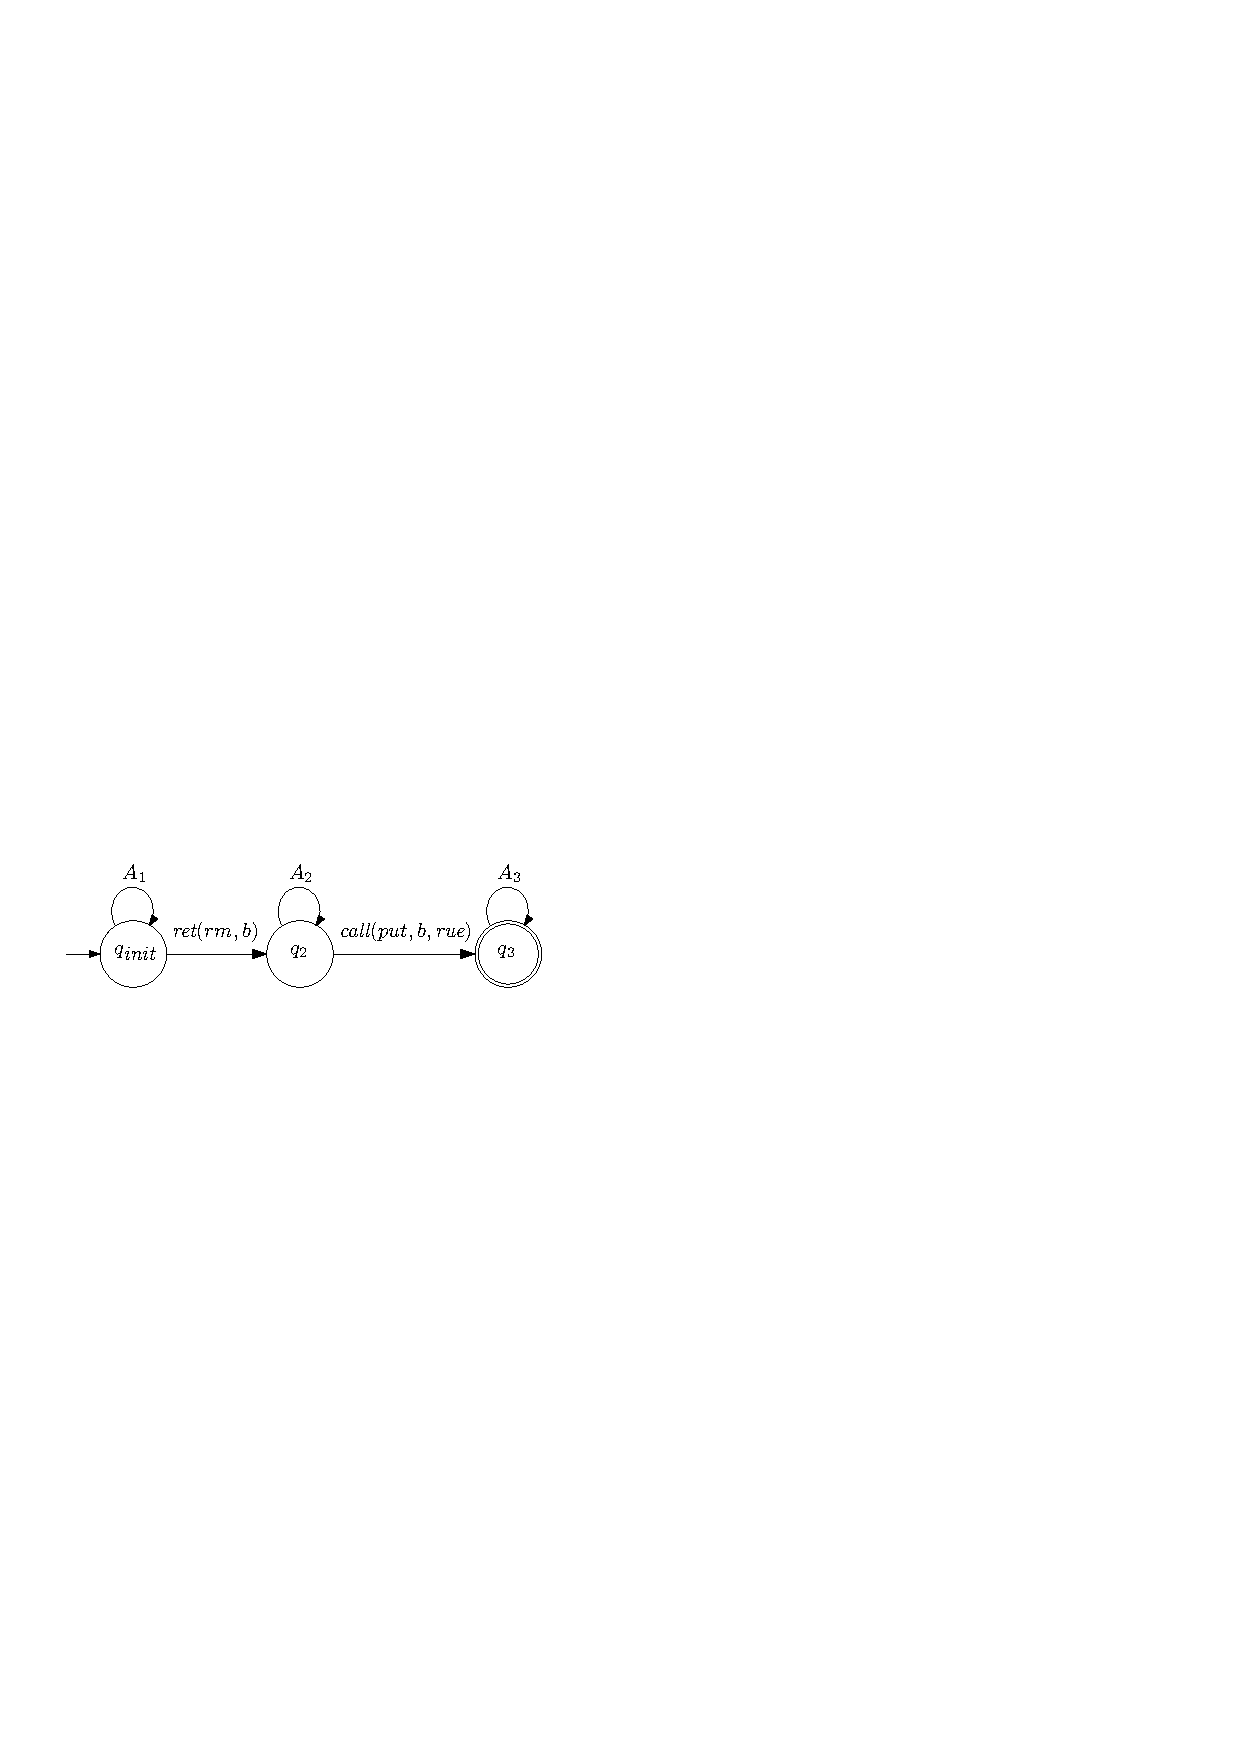
\includegraphics[width=0.5 \textwidth]{figures/PIC_AUTO_FIFO_1.pdf}
%\vspace{-10pt}
  \caption{Automaton $\mathcal{A}_{\textit{SinPri}}^1$}
  \label{fig:automata for FIFO-1 in appendix}
\end{figure}


We generate register automata $\mathcal{A}_{\textit{SinPri}}^2$ for the second case, and it is shown in \figurename~\ref{fig:automata for FIFO-2}. Here $C_1 = \{ \textit{call}(\textit{put},a,\textit{true}),\textit{ret}(\textit{put},a,\textit{true}), \textit{call}(\textit{rm},a),\textit{ret}(\textit{rm},a),\textit{call}(\textit{rm},\textit{empty}),\textit{ret}(\textit{rm},\textit{empty}) \}$, $C_2 = C_1 \cup \{ \textit{call}(\textit{rm},b) + \textit{ret}(\textit{rm},b) \}$.


\begin{figure}[htbp]
  \centering
  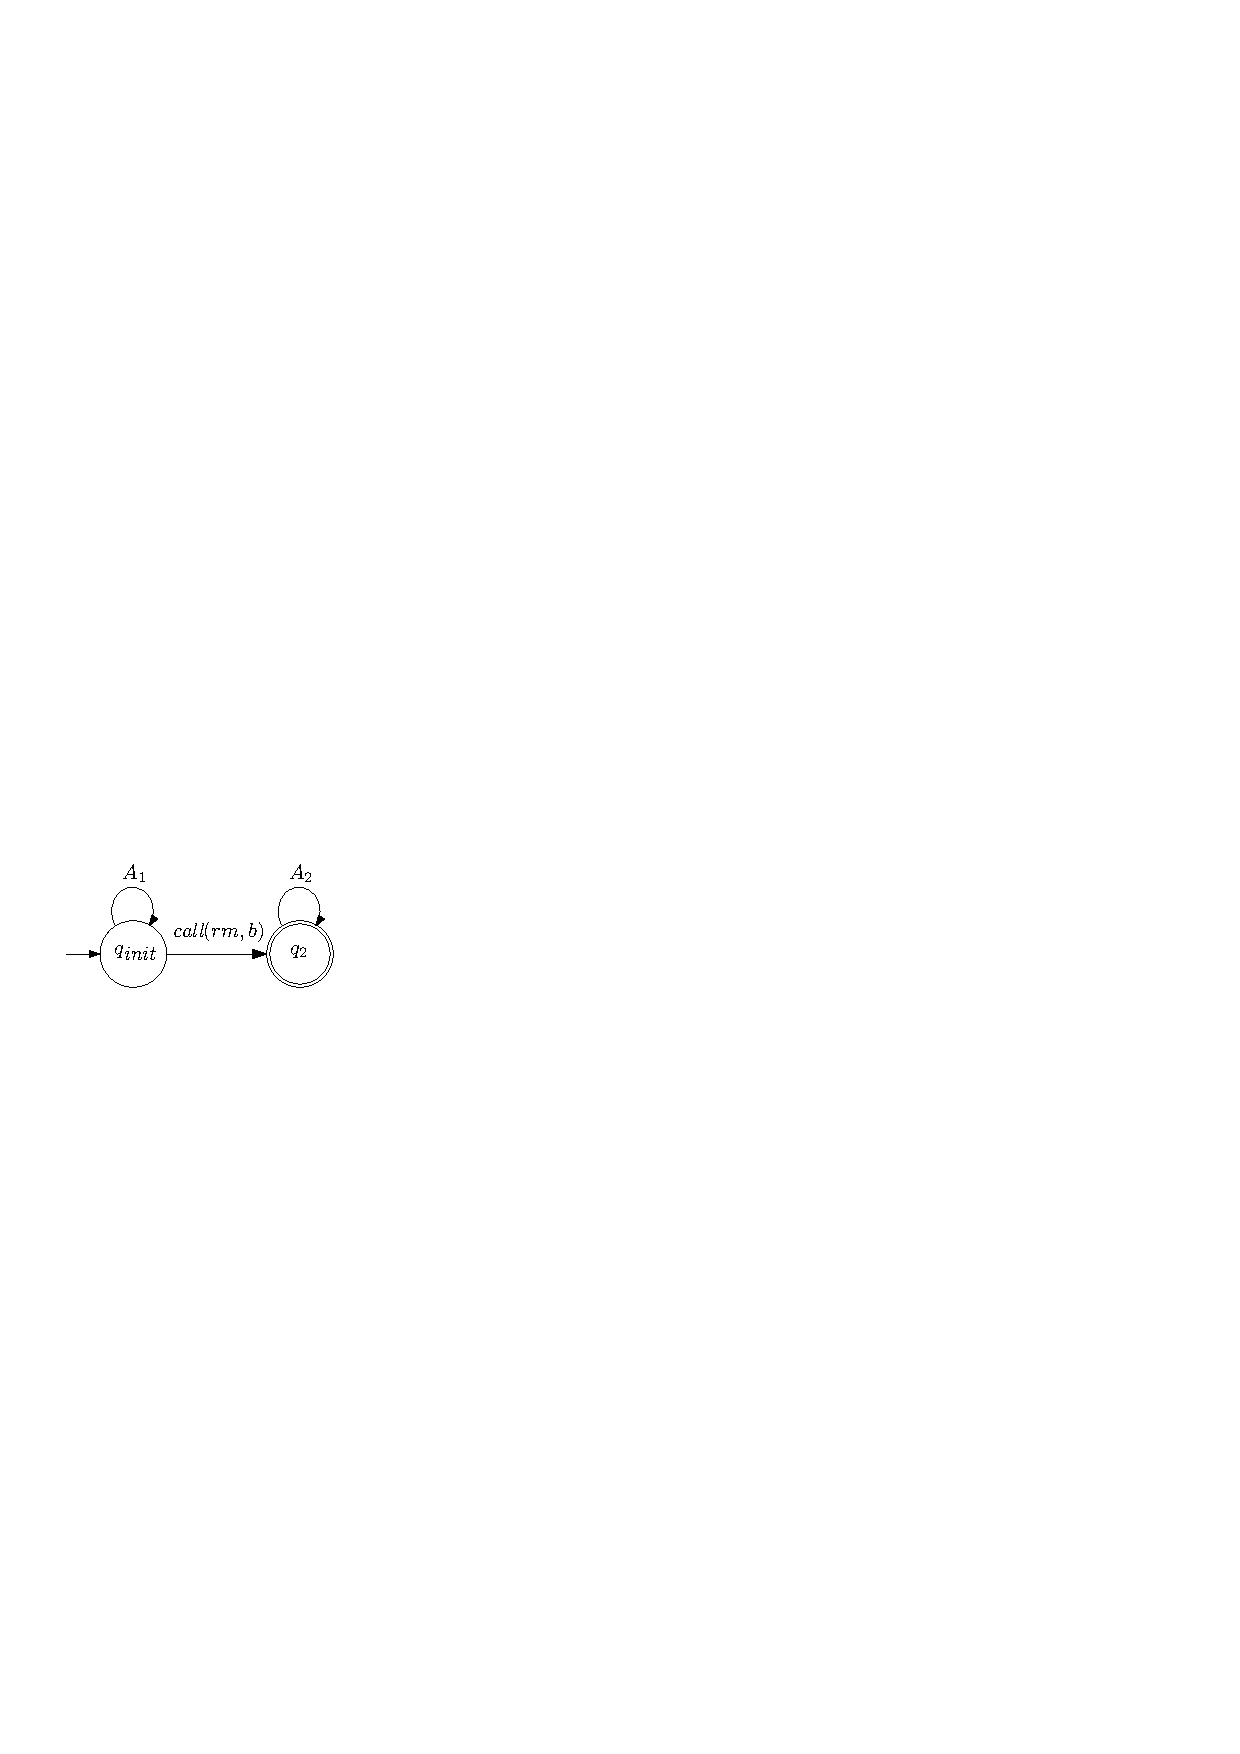
\includegraphics[width=0.3 \textwidth]{figures/PIC_AUTO_FIFO_2.pdf}
%\vspace{-10pt}
  \caption{Automaton $\mathcal{A}_{\textit{SinPri}}^2$}
  \label{fig:automata for FIFO-2}
\end{figure}

We generate register automata $\mathcal{A}_{\textit{SinPri}}^3$ for the third case, and it is shown in \figurename~\ref{fig:automata for FIFO-3}. Here $C_1 = \{ \textit{call}(\textit{put},a,\textit{true}),\textit{ret}(\textit{put},a,\textit{true}), \textit{call}(\textit{rm},a),\textit{ret}(\textit{rm},a),\textit{call}(\textit{rm},\textit{empty}),\textit{ret}(\textit{rm},\textit{empty}) \}$, $C_2 = C_1 \cup \{ \textit{ret}(\textit{put},b,\textit{true}) \}$, $C_3 = C_2 \cup \{ \textit{ret}(\textit{rm},b) \}$, $C_4 = C_3 \cup \{ \textit{call}(\textit{rm},b) \}$, $C_5 = C_1 \cup \{ \textit{ret}(\textit{rm},b) \}$, $C_6 = C_5 \cup \{ \textit{call}(\textit{rm},b) \}$.

\begin{figure}[htbp]
  \centering
  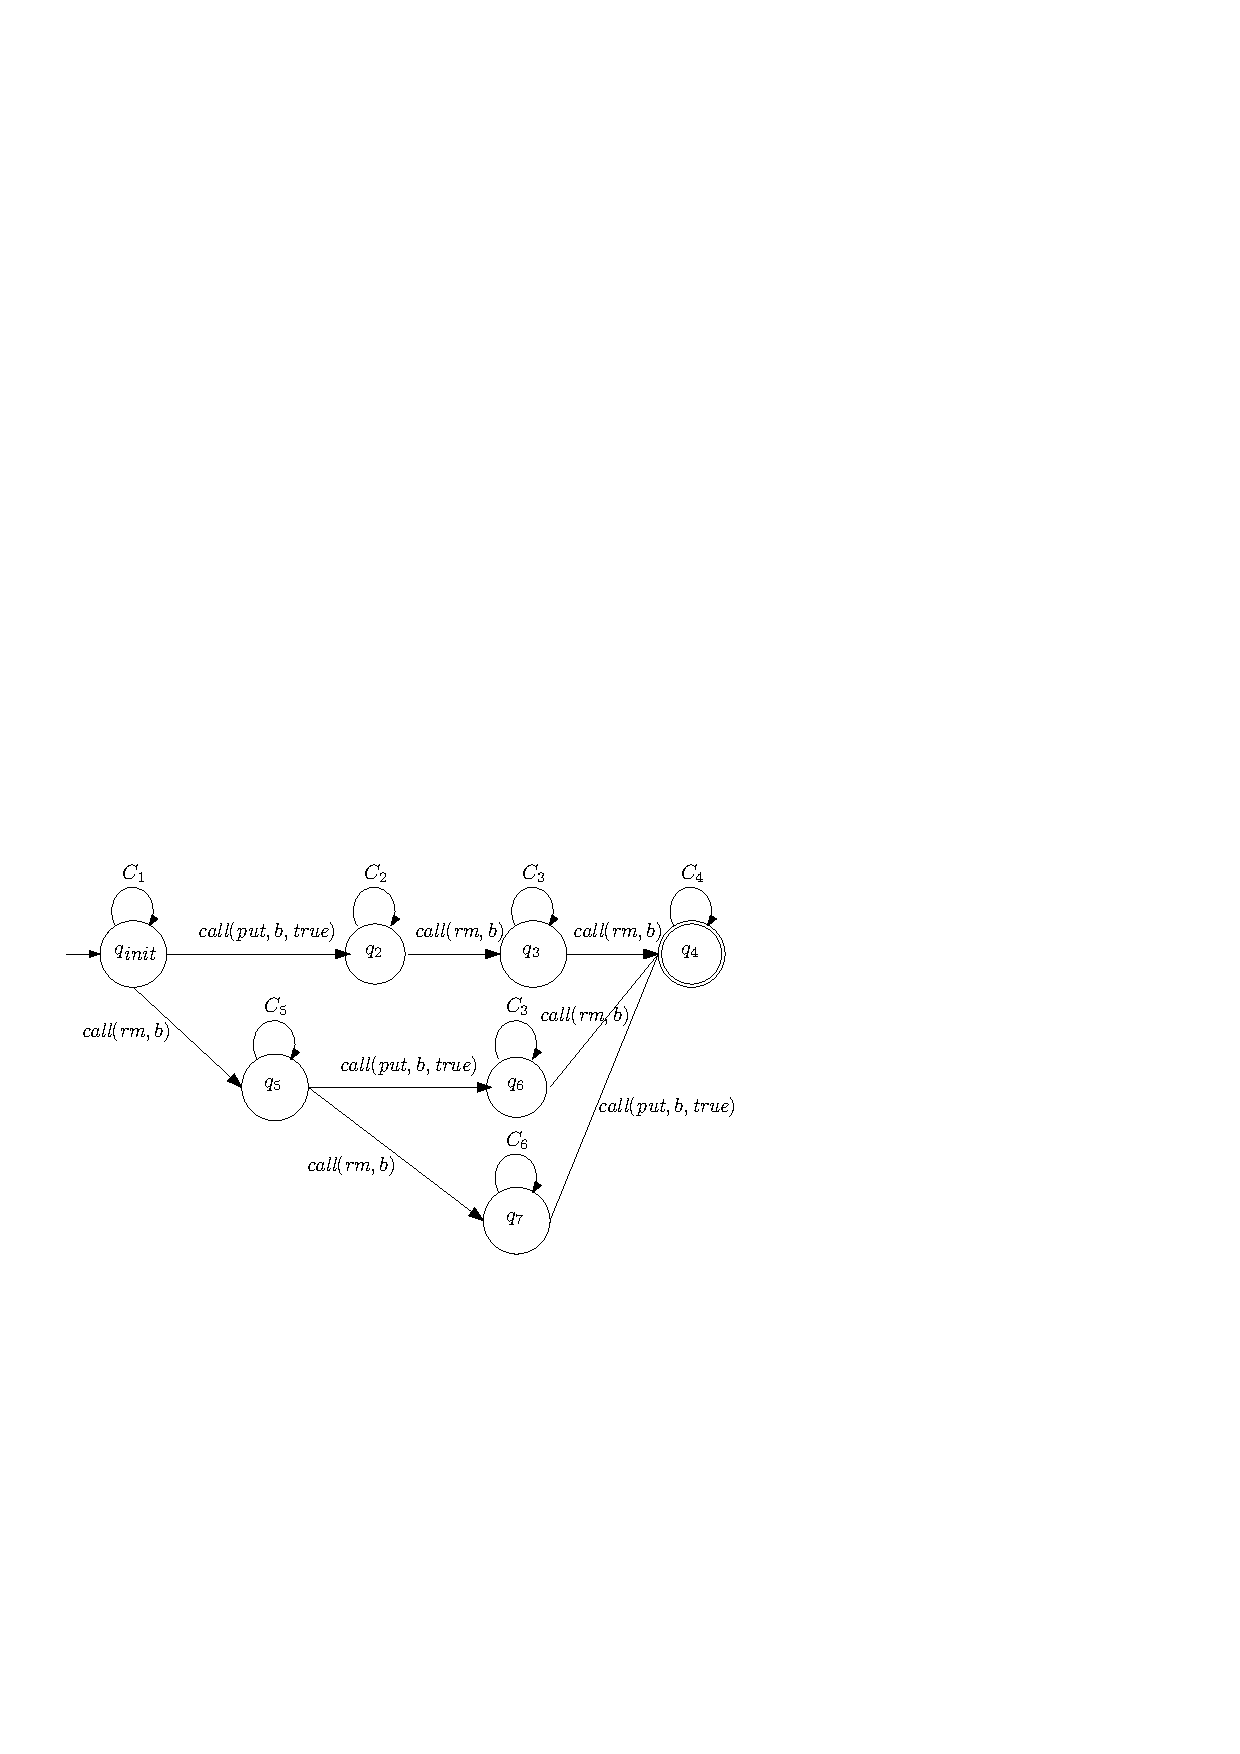
\includegraphics[width=0.7 \textwidth]{figures/PIC_AUTO_FIFO_3.pdf}
%\vspace{-10pt}
  \caption{Automaton $\mathcal{A}_{\textit{SinPri}}^3$}
  \label{fig:automata for FIFO-3}
\end{figure}

We generate register automata $\mathcal{A}_{\textit{SinPri}}^4$ for the forth case, and it is shown in \figurename~\ref{fig:automata for FIFO-4}. Here $C_1 = C \cup \{ \textit{call}(\textit{rm},b) \}$, and $C_2 = C \cup \{ \textit{ret}(\textit{put},b,=r), \textit{call}(\textit{rm},a), \textit{ret}(\textit{rm},a) \}$, where $C = \{ \textit{call}(\textit{put},d,\textit{true}),\textit{ret}(\textit{put},d,\textit{true}), \textit{call}(\textit{rm},d),\textit{ret}(\textit{rm},d),\textit{call}(\textit{rm},\textit{empty}),\textit{ret}(\textit{rm},\textit{empty}) \}$.

\begin{figure}[htbp]
  \centering
  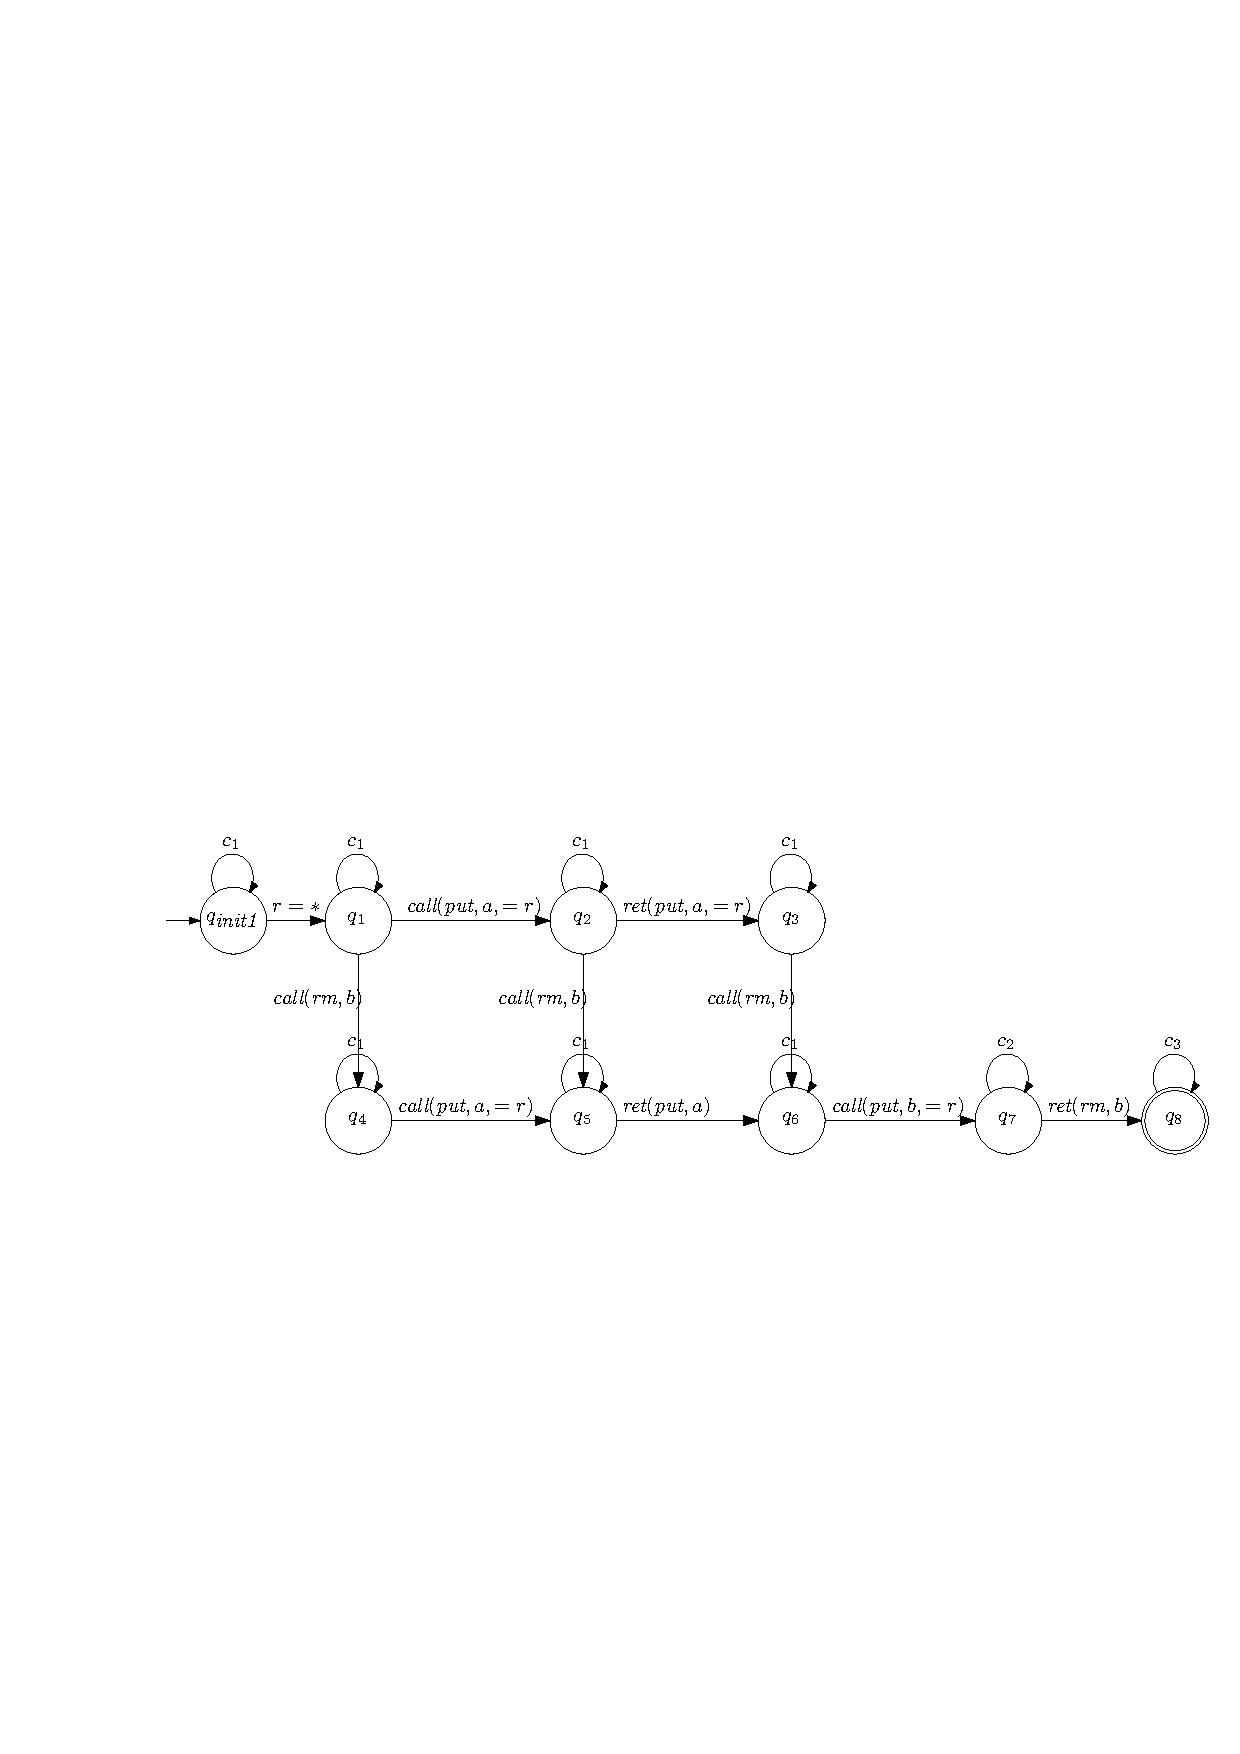
\includegraphics[width=0.9 \textwidth]{figures/PIC_AUTO_FIFO_4.pdf}
%\vspace{-10pt}
  \caption{Automaton $\mathcal{A}_{\textit{SinPri}}^4$}
  \label{fig:automata for FIFO-4}
\end{figure}

Let $\mathcal{A}_{\textit{sinPri}}$ be the union of $\mathcal{A}_{\textit{SinPri}}^1, \mathcal{A}_{\textit{SinPri}}^2, \mathcal{A}_{\textit{SinPri}}^3, \mathcal{A}_{\textit{SinPri}}^4$. Let us prove Lemma \ref{lemma:automata for extended priority queue with single priority}.

\begin{lemma}\label{lemma:automata for extended priority queue with single priority}
Given a data-independent implementations $\mathcal{I}$ of extended priority queue, $\mathcal{I} \cap \mathcal{A}_{\textit{sinPri}} \neq \emptyset$, if and only if there exists $e \in \mathcal{I}_{\neq}$, $e' \in \textit{proj}(e)$, such that $e'$ is single-priority  without $\textit{rm}(\textit{empty})$, and $\textit{transToQueue}(e')$ does not linearizable to queue.
\end{lemma}

%\begin{restatable}{lemma}{AutoForEPQwithSignlePri}
%\label{lemma:automata for extended priority queue with single priority}
%
%Given a data-independent implementations $\mathcal{I}$ of extended priority queue, $\mathcal{I} \cap \textit{Auts}_{\textit{sinPri}} \neq \emptyset$, if and only if there exists $e \in \mathcal{I}_{\neq}$, $e' \in \textit{proj}(e)$, such that $e'$ is single-priority  without $\textit{rm}(\textit{empty})$, and $\textit{toQueue}(e')$ does not linearizable to queue.
%\end{restatable}

%\AutoForEPQwithSignlePri*

\begin {proof}

\cite{DBLP:conf/icalp/BouajjaniEEH15} states that, given a differentiated queue execution $e$ without $\textit{deq}(\textit{empty})$, $e$ is not linearizable with respect to queue, if one of the following cases holds for some $v_a,v_b$: (1) $\textit{deq}(v_b) <_{hb} \textit{enq}(v_b)$, (2) there are are no $\textit{enq}(v_b)$ and at least one $\textit{deq}(v_b)$, (3) there are are one $\textit{enq}(v_b)$ and more than one $\textit{deq}(v_b)$, and (4) $\textit{enq}(v_a) <_{\textit{hb}} \textit{enq}(v_b)$, and $\textit{deq}(v_b) <_{\textit{hb}} \textit{deq}(v_a)$, or $\textit{deq}(v_a)$ does not exists.

Let us prove the $\textit{only if}$ direction. Assume that there exists execution $e_0 \in \mathcal{I}$ and $e_0$ is accepted by $\mathcal{A}_{\textit{SinPri}}^1, \mathcal{A}_{\textit{SinPri}}^2, \mathcal{A}_{\textit{SinPri}}^3$ or $\mathcal{A}_{\textit{SinPri}}^4$. By data-independence, we can see that there exists a data-differentiated $e \in \mathcal{I}$ and renaming function, such that $e_0=r(e)$. Let $e'$ be obtained from $e$ by first removing $\textit{rm}(\textit{empty})$, and then,

\begin{itemize}
\setlength{\itemsep}{0.5pt}
\item[-] If $e_0$ is accepted by $\mathcal{A}_{\textit{SinPri}}^1$, $\mathcal{A}_{\textit{SinPri}}^2$ or $\mathcal{A}_{\textit{SinPri}}^3$: Then remove all items that are not renamed into $b$ by $r$.

\item[-] If $e_0$ is accepted by $\mathcal{A}_{\textit{SinPri}}^4$: Then remove all items that are not renamed into $a$ or $b$ by $r$.
\end{itemize}

It is obvious that $e' \in \textit{proj}(e)$. It is easy to see that $\textit{transToQueue}(e')$ satisfies one of above conditions, and then $\textit{transToQueue}(e')$ is not linearizable w.r.t queue.

Let us prove the $\textit{if}$ direction. Assume that exists $e \in \mathcal{I}_{\neq}$, $e' \in \textit{proj}(e)$, such that $e'$ is single-priority  without $\textit{rm}(\textit{empty})$, and $\textit{transToQueue}(e')$ does not linearizable to queue. Then we construct a renaming function $r$ as follows:

\begin{itemize}
\setlength{\itemsep}{0.5pt}
\item[-] If this is because case $1$, case $2$ or case $3$: $r$ maps $v_b$ into $b$ and maps all other values into $a$.

\item[-] If this is because case $4$: $r$ maps $v_a$ and $v_b$ into $a$ and $b$, respectively, and maps all other values into $d$.
\end{itemize}

Then it is not hard to see that $r(e) \in \mathcal{I}$ and it is accepted by $\mathcal{A}_{\textit{SinPri}}^1, \mathcal{A}_{\textit{SinPri}}^2, \mathcal{A}_{\textit{SinPri}}^3$ or $\mathcal{A}_{\textit{SinPri}}^4$. This completes the proof of this lemma. \qed
\end {proof}




\subsection{Proof of Lemma \ref{lemma:pri execution is enough}}
\label{sec:appendix proof of Lemma pri execution is enough}

The following lemma states that, from linearization of sub-histories, we can merge them and obtain a linearization (regardless of whether it belongs to sequential specification) of the whole history.

\begin{restatable}{lemma}{MergeTwoLinearization}
\label{lemma:merge two linearization}

Given an execution $e$, operation sets $S_1$, $S_2$ and sequences $l_1$ and $l_2$. Let $e_1 = e \vert{S_1}$ and $e_2 = e \vert{S_2}$. Assume that $e_1 \sqsubseteq l_1$, $e_2 \sqsubseteq l_2$, and $S_1 \cup S_2$ contains all operations of $e$. Then, there exists a sequence $l$, such that $e \sqsubseteq l$, $l \vert{S_1} = l_1$ and $l \vert{S_2} = l_2$.
\end{restatable}

\begin {proof}

Given an execution $e$ and a operation $o \in S_2$, let $\textit{MB}(o) = \{ o' \vert o' \in S_1$ and $o'$ happens before $o$ in $h \}$, let $\textit{SBI}(o) = \textit{min}\{ i \vert l_1[0,i]$ contains all elements of $\textit{MB}(o) \}$.

Let $l = s_1 \cdot l_2[1] \cdot \ldots \cdot l_2[n] \cdot s_{\textit{n+1}}$ be generated as follows, where $n = \vert l_2 \vert$:

\begin{itemize}
\setlength{\itemsep}{0.5pt}
\item[-] $s_1 = l_1[0, \textit{SBI}(l_2[1])]$,

\item[-] If $s_1 \cdot l_2[1] \cdot \ldots \cdot l_2[i]$ already contains $l_1(\textit{SBI}(l_2[\textit{i+1}]))$, then $s_{\textit{i+1}} = \epsilon$. Otherwise, $s_{\textit{i+1}}$ is a subsequence of $l_1$, which starts from the next of last elements of $s_1 \cdot l_2[1] \cdot \ldots \cdot l_2[i]$ in $l_1$ and ends in $l_1(\textit{SBI}(l_2[\textit{i+1}]))$.
\end{itemize}

It is obvious that $l \vert{S_1} = l_1$ and $l \vert{S_2} = l_2$, and it remains to prove that $e \sqsubseteq l$. We prove this by contradiction. Assume that $e \not \sqsubseteq l$. Then there must be two operations $o_1$, $o_2$ of $e$, such that $o_1 <_{hb} o_2$ in $e$ but $o_2$ before $0_1$ in $l$. Since $l \vert{S_1} = l_1$, $l \vert{S_2} = l_2$, and $h_1 \sqsubseteq l_1$, $h_2 \sqsubseteq l_2$, it is easy to see that it is impossible that $o_1,o_2 \in S_1$ or $o_1,o_2 \in S_2$. There are only two possibilities:

\begin{itemize}
\setlength{\itemsep}{0.5pt}
\item[-] $o_1 \in S_1 \wedge o_2 \in S_2$. Then we can see that $o_2=l_2[i]$ and $o_1 \in s_j$ for some $i < j$. Since $o_1 <_{hb} o_2$, we know that $o_1 \in \textit{SBI}(o_2)$. By the construction of $l$, we know that $o_1$ must be in $s_k$ for some $k \leq i$, contradicts that $o_1 \in s_j$ with $i < j$.

\item[-] $o_1 \in S_2 \wedge o_2 \in S_1$. Then we can see that $o_2 \in s_i$ and $o_1 = l_2[j]$ for some $i \leq j$. It is easy to see that this leads to contradiction when $i = j$. For the case of $i \neq j$, we need to satisfy the following requirements: (1) $o_1$ ($l_2[j]$) does not happen before $l_2[i]$, (2) $l_2[i]$ does not happen before $o_2$, (3) $o_2$ is either overlap or happens before $o' \in \textit{MB}(l_2[i])$, and (4) $o' <_{hb} l_2[i]$. By enumeration we can see that it is impossible that above four conditions be satisfied while $o_1 <_{hb} o_2$.
\end{itemize}

This completes the proof of this lemma. \qed
\end {proof}

With Lemma \ref{lemma:merge two linearization}, we can now prove Lemma \ref{lemma:pri execution is enough}.

\priExecutionIsEnough*
\begin {proof}

We deal with the case of $\Gamma = \mathsf{MatchedMaxPriority}^{>}$ , and other cases can be similarly dealt with.

To prove the $\textit{only if}$ direction, assume that $e \sqsubseteq l$, $\mathsf{MatchedMaxPriority\text{-}Seq}(l,x)$ holds and $p$ is the priority of $x$. We can see that $e \sqsubseteq u \cdot \textit{put}(x,p) \cdot v \cdot \textit{rm}(x) \cdot w$. Let $u'$, $v'$ and $w'$ be obtained from $u$, $v$ and $w$ by erasing all items with priority incomparable with $p$, respectively. Since the predicates in $\mathsf{MatchedMaxPriority\text{-}Seq}(l,x)$ does not restrict the values of priorities incomparable with $p$, is not hard to see that $e \sqsubseteq l'$ and $\mathsf{MatchedMaxPriority\text{-}Seq}(l',x)$ holds, where $l' = u' \cdot \textit{put}(x,\textit{pri}) \cdot v' \cdot \textit{rm}(x) \cdot w'$.

To prove the $\textit{if}$ direction, given $e' = e \vert_{\prec p}$. By assumption, $e' \sqsubseteq l$, $\mathsf{MatchedMaxPriority\text{-}Seq}(l,x)$ holds and $p$ is the priority of $x$, and then we can see that $e' \sqsubseteq l_1 = u \cdot \textit{put}(x,p) \cdot v \cdot \textit{rm}(x) \cdot w$. Let $O_c$ be the set of operations in $e$ that have priorities comparable with $p$, and Let $O_i$ be the set of operations in $e$ that have priorities incomparable with $p$. It is obvious that $l_1$ is the linearization of $e \vert_{O_c}$. By Lemma \ref{lemma:merge two linearization}, there exists sequence $l$, such that $e \sqsubseteq l$, and $l \vert_{O_c} = l_1$. Then $l = u' \cdot \textit{put}(x,p) \cdot v' \cdot \textit{rm}(x) \cdot w'$, where $u' \vert_{O_c} = u$, $v' \vert_{O_c} = v$ and $w' \vert_{O_c} = w$. Since $p$ is one of maximal priorities in $e$, and the predicates in $\mathsf{MatchedMaxPriority\text{-}Seq}(l,x)$ does not restrict the values with priority $O_i$, it is easy to see that $\mathsf{MatchedMaxPriority\text{-}Seq}(l,x)$ holds. \qed
\end {proof}

Therefore, from now on, it is safe to consider only the data-differentiated sequences with only one maximal priority. 





\subsection{Proofs, Definitions and Register Automata in Subsection \ref{subsec:co-regular of EPQ1Lar}}
\label{sec:appendix proof and definition in section co-regular of EPQ1Lar}


Let us introduce $\textit{UVSet}(e,x)$, which intuitively contains all pairs of operations that should be putted before $\textit{rm}(x)$ when construction linearization of $x$ according to $\mathsf{MatchedMaxPriority}$. Let $\textit{UVSet}_1(e$, $x) = o \vert$ either $o <{\textit{hb}} \textit{put}(x,\_)$ or $\textit{rm}(x)$, or there exists $o'$ with the same value of $o$, such that $o' <{\textit{hb}} \textit{put}(x)$ or $\textit{rm}(x) \}$. For each $i > 1$, let $\textit{UVSet}_{\textit{i+1}}(e,x) = o \vert$ $o \notin \textit{UVSet}_k$ for each $k \leq i$, and either $o$ happens before some operation $o' \in \textit{UVSet}_i(e,x)$, or there exists $o''$ with the same value of $o$, and $o''$ happens before some operation $o' \in \textit{UVSet}_i(e,x) \}$. Let $\textit{UVSet}(e,x) = \textit{UVSet}_1(e,x) \cup \ldots$. Note that it is possible that $\textit{UVSet}_i(e,x) \cap \textit{UVSet}_j(e,x) = \emptyset$ for any $i \neq j$.

The following lemma states that $\textit{UVSet}(e,x)$ contains only matched $\textit{put}$ and $\textit{rm}$.

\begin{restatable}{lemma}{UVSetHasMatchedPutandRm}
\label{lemma:UVSet has matched put and rm}
Given a data-differentiated execution $e$ where $\mathsf{Has\text{-}MatchedMaxPriority}(e)$ holds, let $p$ be its maximal priority and $\textit{put}(x,p),\textit{rm}(x)$ are only operations of priority $p$ in $e$. Let $G$ be the graph representing the left-right constraint of $x$. Assume that $G$ has no cycle going through $x$. Then, $\textit{UVSet}(e,x)$ contains only matched $\textit{put}$ and $\textit{rm}$.
\end{restatable}
\begin {proof}

We prove this lemma by contradiction. Assume that there exists a value, such that $\textit{UVSet}(e,x)$ contains only its $\textit{put}$ and does not contain its $\textit{rm}$. Then we can see that there exists $d_1,\ldots,d_j$. Intuitively, $d_1,\ldots,d_j$ are elements in $\textit{UVSet}_1(e,x), \ldots, \textit{UVSet}_i(e,x)$, respectively. $\textit{UVSet}(e,x)$ contains $\textit{put}(d_j,\_)$ and does not contain $\textit{rm}(d_j)$. And each $d_i$ is the reason of $d_{\textit{i+1}} \in \textit{UVSet}_{\textit{i+1}}(e,x)$. Formally, we require that

\begin{itemize}
\setlength{\itemsep}{0.5pt}
\item[-] For each $1 \leq i \leq j$, operations of $d_i$ belongs to $\textit{UVSet}_i(e,x)$.

\item[-] For each $i \neq j$, $\textit{put}(d_i,\_),\textit{rm}(d_i) \in \textit{UVSet}_i(e,x)$. $\textit{put}(d_j,\_) \in \textit{UVSet}_j(e,x)$, and $e$ does not contain $\textit{rm}(d_j)$.

\item[-] An operation of $d_1$ happens before an operations of $x$. For each $1 < i \leq j$, an operation of $d_i$ happens an operation of $d_{\textit{i-1}}$.

\item[-] For each $k$ and $\textit{ind}$, if $k > \textit{ind+1}$, then no operation of $d_k$ happens before operation of $d_{\textit{ind}}$.
\end{itemize}

According to the definition of $\textit{UVSet}(e,x)$, it is easy to see that such $d_1,\ldots,d_j$ exists. Let us prove the following fact:

\noindent {\bf $\textit{fact}_1$}: Given $1 \leq i < j$, it can not be the case that $\textit{put}(d_i,\_)$ and $\textit{rm}(d_i)$ overlap.

Proof of $\textit{fact}_1$: We prove $\textit{fact}_1$ by contradiction. Assume that for some $i \neq j$, $\textit{put}(d_i,\_)$ and $\textit{rm}(d_i)$ overlap. Since $\textit{put}(d_i,\_), \textit{rm}(d_i) \in \textit{UVSet}_i(h,x)$, we know that an operation $o_i$ of $d_i$ happens before operation $o_{\textit{i-1}}$ of $d_{\textit{i-1}}$. Moreover, since $\textit{put}(d_i,\_)$ and $\textit{rm}(d_i)$ overlap, it is not hard to see that the call action of $\textit{put}(d_i,\_)$ and the call action of $\textit{rm}(d_i)$ is before the call action of $o_{\textit{i-1}}$. Since operations of $d_{\textit{i+1}}$ is in $\textit{UVSet}_{\textit{i+1}}(e,x)$, we know that an operation $o'_{\textit{i+1}}$ of $d_{\textit{i+1}}$ happens before operation $o'_i$ of $d_i$. Then, it is not hard to see that $o'_{\textit{i+1}}$ also happens before $o_{\textit{i-1}}$, which contradicts that for each $k > \textit{ind+1}$, no operation of $d_k$ happens before operation of $d_{\textit{ind}}$.

We already know that an operation of $d_1$ happens before an operation of $x$. By $\textit{fact}_1$, we can ensure that $\textit{put}(d_1,\_)$ happens before an operation of $x$, and then $d_1 \rightarrow x$ in $G$. For each $1 < i \leq j$, we know that an operation $o_i$ of $d_i$ happens before an operation $o_{\textit{i-1}}$ of $d_{\textit{i-1}}$. By $\textit{fact}_1$, we can ensure that $o_i=\textit{put}(d_i,\_)$ and $o_{\textit{i-1}}=\textit{rm}(d_{\textit{i-1}})$, and then $d_i \rightarrow d_{\textit{i-1}}$ in $G$. Since $h$ contains $\textit{put}(d_j,\_)$ and does not contain $\textit{rm}(d_j)$, we know that $x \rightarrow d_j$ in $G$. Then $G$ has a cycle going through $x$, contradicts that $G$ has no cycle going through $x$. \qed
\end {proof}


The following lemma states that $\textit{UVSet}(e,x)$ does not happen before $\textit{rm}(x)$ when the left-right constraint has no cycle going through $x$.

\begin{restatable}{lemma}{RmxDoesNotHappenBeforeUVSetForEPQ1Lar}
\label{lemma:Rmx does not happen before UVSet for EPQ1Lar}

Given a data-differentiated execution $e$ where $\mathsf{Has\text{-}MatchedMaxPriority}(e)$ holds, let $p$ be its maximal priority and $\textit{put}(x,p),\textit{rm}(x)$ are only operations of priority $p$ in $e$. Let $G$ be the graph representing the left-right constraint of x. Assume that $G$ has no cycle going through $x$. Then, $\textit{rm}(x)$ does not happen before any operation in $\textit{UVSet}(e,x)$.
\end{restatable}

\begin {proof}

We prove this lemma by induction, and prove that $\textit{rm}(x)$ does not happen before any operation in $\textit{UVSet}_1(e,x)$, in $\textit{UVSet}_2(e,x)$, $\ldots$. Note that, by Lemma \ref{lemma:UVSet has matched put and rm}, $\textit{UVSet}(e,x)$ contains only matched $\textit{put}$ and $\textit{rm}$, and it is easy to see that for each $i$, $\textit{UVSet}_i(e,x)$ contains only matched $\textit{put}$ and $\textit{rm}$.

\noindent (1) Let us prove that $\textit{rm}(x)$ does not happen before any operation in $\textit{UVSet}_1(e,x)$ by contradiction. Assume that $\textit{rm}(x) <_{hb} o$, where $o \in \textit{UVSet}_1(e,x)$ is an operation of item $d$. 

We use a triple $(t_1,t_2,t_3)$ to represent related information. $t_1,t_2,t_3$ are chosen from $\{ \textit{put},\textit{rm} \}$. $t_1$ represents whether $o$ is a $\textit{put}$ operation or a $\textit{rm}$ operation. $t_2$ and $t_3$ is used for the reason of $o \in \textit{UVSet}_1(e,x)$: $o \in \textit{UVSet}_1(e,x)$, since an operation (of kind $t_2$) of $d$ happens before an operation (of kind $t_3$) of $x$. Let us consider all the possible cases of $(t_1,t_2,t_3)$:

\begin{itemize}
\setlength{\itemsep}{0.5pt}
\item[-] $(\textit{put},\textit{put},\textit{put})$: Then $\textit{rm}(x) <_{hb} \textit{put}(d,\_) <_{hb} \textit{put}(x,p)$, contradicts that $\textit{rm}(x)$ does not happen before $\textit{put}(x,p)$.

\item[-] $(\textit{put},\textit{put},\textit{rm})$: Then $\textit{rm}(x) <_{hb} \textit{put}(d,\_) <_{hb} \textit{rm}(x)$, contradicts that $\textit{rm}(x)$ does not happen before $\textit{rm}(x)$.

\item[-] $(\textit{put},\textit{rm},\textit{put})$: Then $( \textit{rm}(x) <_{hb} \textit{put}(d,\_) ) \wedge ( \textit{rm}(d) <_{hb} \textit{put}(x,p) )$. By interval order, we know that $( \textit{rm}(x) <_{hb} \textit{put}(x,p) ) \vee ( \textit{rm}(d) <_{hb} \textit{put}(d,\_) )$, which is impossible.

\item[-] $(\textit{put},\textit{rm},\textit{rm})$: Then $( \textit{rm}(x) <_{hb} \textit{put}(d,\_) ) \wedge ( \textit{rm}(d) <_{hb} \textit{rm}(x) )$. We can see that $\textit{rm}(d) <_{hb} \textit{rm}(x) <_{hb} \textit{put}(d,\_)$, which contradicts that $\textit{rm}(d)$ does not happen before $\textit{put}(d,\_)$.

\item[-] $(\textit{rm},\textit{put},\textit{put})$: Then $( \textit{rm}(x) <_{hb} \textit{rm}(d) ) \wedge ( \textit{put}(d,\_) <_{hb} \textit{put}(x,p) )$. We can see that $x$ and $d$ has circle in $G$, contradicts that $G$ has no cycle going through $x$.

\item[-] $(\textit{rm},\textit{put},\textit{rm})$: Then $( \textit{rm}(x) <_{hb} \textit{rm}(d) ) \wedge ( \textit{put}(d,\_) <_{hb} \textit{rm}(x) )$. We can see that $x$ and $d$ has circle in $G$, contradicts that $G$ has no cycle going through $x$.

\item[-] $(\textit{rm},\textit{rm},\textit{put})$: Then $\textit{rm}(x) <_{hb} \textit{rm}(d) <_{hb} \textit{put}(x,p)$, contradicts that $\textit{rm}(x)$ does not happen before $\textit{put}(x,p)$.

\item[-] $(\textit{rm},\textit{rm},\textit{rm})$: Then $\textit{rm}(x) <_{hb} \textit{rm}(d) <_{hb} \textit{rm}(x)$, contradicts that $\textit{rm}(x)$ does not happen before $\textit{rm}(x)$.
\end{itemize}

This completes the proof for $\textit{UVSet}_1(e,x)$.

\noindent (2) Assume we already prove that for some $j \geq 1$, $\textit{rm}(x)$ does not happen before any operation in $\textit{UVSet}_1(e,x) \cup \ldots \cup \textit{UVSet}_j(e,x)$. Let us prove that $\textit{rm}(x)$ does not happen before any operation in $\textit{UVSet}_{\textit{j+1}}(e,x)$ by contradiction. Assume that $\textit{rm}(x) <_{hb} o$, where $o \in \textit{UVSet}_{\textit{j+1}}(e,x)$ is an operation of item $d_{\textit{j+1}}$. We use a triple $(t_1,t_2,t_3)$ to represent related information. $t_1,t_2,t_3$ are chosen from $\{ \textit{put},\textit{rm} \}$. $t_1$ represents whether $o$ is a $\textit{put}$ operation or a $\textit{rm}$ operation. $t_2$ and $t_3$ is used for the reason of $o \in \textit{UVSet}_{\textit{j+1}}(e,x)$: $o \in \textit{UVSet}_{\textit{j+1}}(e,x)$, since an operation (of kind $t_2$) of $d_{\textit{j+1}}$ happens before an operation (of kind $t_3$) of $d_j$, where $\textit{put}(d_j,\_), \textit{rm}(d_j) \in \textit{UVSet}_j(e,x)$. Let us consider all the possible cases of $(t_1,t_2,t_3)$:

\begin{itemize}
\setlength{\itemsep}{0.5pt}
\item[-] $(\textit{put},\textit{put},\textit{put})$: Then $\textit{rm}(x) <_{hb} \textit{put}(d_{\textit{j+1}},\_) <_{hb} \textit{put}(d_j,\_)$. We can see that $( \textit{rm}(x) <_{hb} \textit{put}(d_j,\_) ) \wedge ( \textit{put}(d_j,\_) \in \textit{UVSet}_j(e,x) )$, which contradicts that $\textit{rm}(x)$ does not happen before any operation in $\textit{UVSet}_1(e,x) \cup \ldots \cup \textit{UVSet}_j(e,x)$.

\item[-] $(\textit{put},\textit{put},\textit{rm})$: Then $\textit{rm}(x) <_{hb} \textit{put}(d_{\textit{j+1}},\_) <_{hb} \textit{rm}(d_j,\_)$. We can see that $( \textit{rm}(x) <_{hb} \textit{rm}(d_j,\_) ) \wedge ( \textit{rm}(d_j) \in \textit{UVSet}_j(e,x) )$, which contradicts that $\textit{rm}(x)$ does not happen before any operation in $\textit{UVSet}_1(e,x) \cup \ldots \cup \textit{UVSet}_j(e,x)$.

\item[-] $(\textit{put},\textit{rm},\textit{put})$: Then $( \textit{rm}(x) <_{hb} \textit{put}(d_{\textit{j+1}},\_) ) \wedge ( \textit{rm}(d_{\textit{j+1}}) <_{hb} \textit{put}(d_j,\_) )$. By interval order, we know that $( \textit{rm}(x) <_{hb} \textit{put}(d_j,\_) ) \vee ( \textit{rm}(d_{\textit{j+1}}) <_{hb} \textit{put}(d_{\textit{j+1}},\_) )$, which is impossible.

\item[-] $(\textit{put},\textit{rm},\textit{rm})$: Then $( \textit{rm}(x) <_{hb} \textit{put}(d_{\textit{j+1}},\_) ) \wedge ( \textit{rm}(d_{\textit{j+1}}) <_{hb} \textit{rm}(d_j) )$. By interval order, we know that $( \textit{rm}(x) <_{hb} \textit{rm}(d_j) ) \vee ( \textit{rm}(d_{\textit{j+1}}) <_{hb} \textit{put}(d_{\textit{j+1}},\_) )$, which is impossible.

\item[-] $(\textit{rm},\textit{put},\textit{put})$: Then $( \textit{rm}(x) <_{hb} \textit{rm}(d_{\textit{j+1}}) ) \wedge ( \textit{put}(d_{\textit{j+1}},\_) <_{hb} \textit{put}(d_j,\_) )$. Let us consider the reason of $\textit{put}(d_j,\_), \textit{rm}(d_j) \in \textit{UVSet}_j(e,x)$:
    \begin{itemize}
    \setlength{\itemsep}{0.5pt}
    \item[-] If $( j > 1 ) \wedge ( \textit{put}(d_j,\_) <_{hb} o'' )$, where $o''$ is an operation of item $d_{\textit{j-1}}$ and $\textit{put}(d_{\textit{j-1}},\_), \textit{rm}(d_{\textit{j-1}}) \in \textit{UVSet}_{\textit{j-1}}(e,x)$: Then since $( \textit{put}(d_{\textit{j+1}},\_) <_{hb} \textit{put}(d_j,\_) ) \wedge ( \textit{put}(d_j,\_) <_{hb} o'' )$, we can see that $\textit{put}(d_{\textit{j+1}},\_) <_{hb} o''$, and then operations of $d_{\textit{j+1}}$ is in $\textit{UVSet}_j(e,x)$, contradicts that operations of $d_{\textit{j+1}}$ is in $\textit{UVSet}_{\textit{j+1}}(e,x)$.

    \item[-] If $( j = 1 ) \wedge ( \textit{put}(d_j,\_) <_{hb} o'' )$, where $o''$ is an operation of $x$: Similar to above case.

    \item[-] If $( j > 1 ) \wedge ( \textit{rm}(d_j) <_{hb} o'' )$, where $o''$ is an operation of item $d_{\textit{j-1}}$ and $\textit{put}(d_{\textit{j-1}},\_), \textit{rm}(d_{\textit{j-1}}) \in \textit{UVSet}_{\textit{j-1}}(e,x)$: Then since $( \textit{put}(d_{\textit{j+1}},\_) <_{hb} \textit{put}(d_j,\_) ) \wedge ( \textit{rm}(d_j) <_{hb} o'' )$, we can see that $( \textit{put}(d_{\textit{j+1}},\_) <_{hb} o'' ) \vee ( \textit{rm}(d_j) <_{hb} \textit{put}(d_j,\_) )$, which is impossible.

    \item[-] If $( j > 1 ) \wedge ( \textit{rm}(d_j) <_{hb} o'' )$, where $o''$ is an operation of $x$: Similar to above case.
    \end{itemize}

\item[-] $(\textit{rm},\textit{put},\textit{rm})$: Let $T_{\textit{ind}}$ be the set of sentences $\{ \textit{rm}(x) <_{hb} \textit{rm}(d_{\textit{j+1}}), \textit{put}(d_{\textit{j+1}},\_) <_{hb} \textit{rm}(d_j),\ldots, \textit{put}(d_{\textit{ind+1}},\_) <_{hb} \textit{rm}(d_{\textit{ind}}) \}$. Here each $d_i$ is a item of some operation in $\textit{UVSet}_i(e,x)$. Let us prove that from $T_j$ we can obtain contradiction by induction:

    {\bf Base case $1$}: From $T_1$ we can obtain contradiction.

    Let us prove base case $1$:

    \begin{itemize}
    \setlength{\itemsep}{0.5pt}
    \item[-] If $\textit{put}(d_1,\_)$ happens $o$, and $o$ is an operation of $x$. Then there is a cycle $x \rightarrow d_{\textit{j+1}} \rightarrow \ldots \rightarrow d_1 \rightarrow x$ in $G$, contradicts that $G$ has no cycle going through $x$.

    \item[-] If $\textit{rm}(d_1)$ happens before $o$, and $o$ is an operation of $x$. Then since $\textit{put}(d_2,\_) <_{hb} \textit{rm}(d_1)$ and $\textit{rm}(d_1) <_{hb} o$, we can see that $\textit{put}(d_2,\_) <_{hb} o$, and then $\textit{put}(d_2,\_) \in \textit{UVSet}_1(e,x)$, contradicts that $\textit{put}(d_2,\_) \in \textit{UVSet}_2(e,x)$.
    \end{itemize}

    {\bf Base case $2$}: From $T_2$ we can obtain contradiction.

    Let us prove base case $2$: If $\textit{rm}(d_2) <_{hb} o$, and $o$ is an operation of $d_1$, then since $( \textit{put}(d_3,\_) <_{hb} \textit{rm}(d_2) ) \wedge ( \textit{rm}(d_2) <_{hb} o )$, we know that $\textit{put}(d_3,\_) <_{hb} o$. This implies that $\textit{put}(d_3,\_) \in \textit{UVSet}_2(e,x)$, contradicts that $\textit{rm}(d_3,\_) \in \textit{UVSet}_3(e,x)$. Therefore, it is only possible that $\textit{put}(d_2,\_)$ happens before an operation of $d_1$.

    \begin{itemize}
    \setlength{\itemsep}{0.5pt}
    \item[-] If $\textit{put}(d_2,\_) <_{hb} \textit{put}(d_1,\_)$ and $\textit{put}(d_1,\_)$ happens before operations of $x$, then we know that $\textit{put}(d_2,\_)$ happens before operation of $x$, which is impossible.

    \item[-] If $\textit{put}(d_2,\_) <_{hb} \textit{put}(d_1,\_)$ and $\textit{rm}(d_1)$ happens before operations of $x$, then by interval order, we know that $\textit{put}(d_2,\_)$ happens before operation of $x$, or $\textit{rm}(d_1) <_{hb} \textit{put}(d_1,\_)$, which is impossible.

    \item[-] If $\textit{put}(d_2,\_) <_{hb} \textit{rm}(d_1)$ and $\textit{put}(d_1,\_)$ happens before operations of $x$, then $x \rightarrow d_{\textit{j+1}} \rightarrow \ldots \rightarrow d_1 \rightarrow x$ in $G$, contradicts that $G$ has no cycle going through $x$.

    \item[-] If $\textit{put}(d_2,\_) <_{hb} \textit{rm}(d_1)$ and $\textit{rm}(d_1)$ happens before operations of $x$, then we know that $\textit{put}(d_2,\_)$ happens before operation of $x$, which is impossible.
    \end{itemize}

    {\bf induction step}: Given $\textit{ind} \geq 3$, if from $T_{\textit{ind-1}}$ we can obtain contradiction, then from $T_{\textit{ind}}$ we can also contain contradiction.


    Prove of the induction step: Similarly as base case $2$, we can prove that it is only possible that $\textit{put}(d_{\textit{ind}},\_)$ happens before operations of $d_{\textit{ind-1}}$.

    \begin{itemize}
    \setlength{\itemsep}{0.5pt}
    \item[-] If $\textit{put}(d_{\textit{ind}},\_) <_{hb} \textit{put}(d_{\textit{ind-1}},\_)$ and $\textit{put}(d_{\textit{ind-1}},\_)$ happens before operations of $d_{\textit{ind-2}}$, then we know that $\textit{put}(d_{\textit{ind}})$ happens before operation of $d_{\textit{ind-2}}$, which is impossible.

    \item[-] If $\textit{put}(d_{\textit{ind}},\_) <_{hb} \textit{put}(d_{\textit{ind-1}},\_)$ and $\textit{rm}(d_{\textit{ind-1}})$ happens before operations of $d_{\textit{ind-2}}$, then by interval order, we know that $\textit{put}(d_{\textit{ind}},\_)$ happens before operation of $d_{\textit{ind-2}}$, or $\textit{rm}(d_{\textit{ind-1}}) <_{hb} \textit{put}(d_{\textit{ind-1}},\_)$, which is impossible.

    \item[-] If $\textit{put}(d_{\textit{ind}},\_) <_{hb} \textit{rm}(d_{\textit{ind-1}})$, then we obtain $T_{\textit{ind-1}}$, which already contain contradiction.
    \end{itemize}

    By base case $1$, base case $2$ and the induction step, it is easy to see that for each $i$, $T_i$ contains contradiction. Therefore, $T_j$, the case of $(\textit{rm},\textit{put},\textit{rm})$, contains contradiction.

\item[-] $(\textit{rm},\textit{rm},\textit{put})$: Then $( \textit{rm}(x) <_{hb} \textit{rm}(d_{\textit{j+1}}) ) \wedge ( \textit{rm}(d_{\textit{j+1}}) <_{hb} \textit{put}(d_j,\_) )$. We can see that $( \textit{rm}(x) <_{hb} \textit{put}(d_j,\_) ) \wedge ( \textit{put}(d_j,\_) \in \textit{UVSet}_j(e,x) )$, which contradicts that $\textit{rm}(x)$ does not happen before any operation in $\textit{UVSet}_1(e,x) \cup \ldots \cup \textit{UVSet}_j(e,x)$.

\item[-] $(\textit{rm},\textit{rm},\textit{rm})$: Then $( \textit{rm}(x) <_{hb} \textit{rm}(d_{\textit{j+1}}) ) \wedge ( \textit{rm}(d_{\textit{j+1}}) <_{hb} \textit{rm}(d_j) )$. We can see that $( \textit{rm}(x) <_{hb} \textit{rm}(d_j) ) \wedge ( \textit{rm}(d_j) \in \textit{UVSet}_j(e,x) )$, which contradicts that $\textit{rm}(x)$ does not happen before any operation in $\textit{UVSet}_1(e,x) \cup \ldots \cup \textit{UVSet}_j(e,x)$.
\end{itemize}

This completes the proof for $\textit{UVSet}_{\textit{j+1}}(e,x)$. Therefore, $\textit{rm}(x)$ does not happen before any operation in $\textit{UVSet}(e,x) = \textit{UVSet}_1(e,x) \cup \textit{UVSet}_2(e,x) \cup \ldots$. \qed
\end {proof}

With Lemma \ref{lemma:UVSet has matched put and rm} and Lemma \ref{lemma:Rmx does not happen before UVSet for EPQ1Lar}, we can now prove Lemma \ref{lemma:Lin Equals Constraint for EPQ1Lar}, which give the equivalent characterization of non $\mathsf{MatchedMaxPriority}$-linearizable executions. 

\begin{restatable}{lemma}{LinEqualsConstraintforEPQOneLar}
\label{lemma:Lin Equals Constraint for EPQ1Lar}
Given a data-differentiated execution $e$ where $\mathsf{Has\text{-}MatchedMaxPriority}(e)$ holds, let $p$ be its maximal priority and $\textit{put}(x,p),\textit{rm}(x)$ are only operations of priority $p$ in $e$. Let $G$ be the graph representing the left-right constraint of $x$. $e$ is $\mathsf{MatchedMaxPriority}$-linearizable, if and only if $G$ has no cycle going through $x$. 
\end{restatable}

\begin {proof}

To prove the $\textit{only if}$ direction, assume that $e \sqsubseteq l$ and $\mathsf{MatchedMaxPriority\text{-}Seq}(l,x)$ holds. Then $l = u \cdot \textit{put}(x,p) \cdot v \cdot \textit{rm}(x) \cdot w$, and let $U$, $V$ and $W$ be the set of operations of $u$, $v$ and $w$, respectively. Assume by contradiction that, there is a cycle $d_1 \rightarrow d_2 \rightarrow \ldots \rightarrow d_m \rightarrow x \rightarrow d_1$ in $G$. It is obvious that the priority of each $d_i$ is smaller than $p$. Then our proof proceeds as follows:

According to the definition of left-right constraint, there are two possibilities. The first possibility is that, $\textit{rm}(x)$ happens before $\textit{rm}(d_1)$. It is obvious that $\textit{rm}(d_1) \in W$, and then since $U \cup V$ contains matched $\textit{put}$ and $\textit{rm}$, we can see that $\textit{put}(d_1),\textit{rm}(d_1) \in W$. Then,

\begin{itemize}
\setlength{\itemsep}{0.5pt}
\item[-] Since $d_1 \rightarrow d_2$, by definition of $G$, we know that $\textit{put}(d_1)$ happens before $\textit{rm}(d_2)$. Since $\textit{put}(d_1) \in W$ and $U \cup V$ contains matched $\textit{put}$ and $\textit{rm}$, we know that $\textit{put}(d_2),\textit{rm}(d_2) \in W$. Similarly, for each $1 \leq i \leq m$, we know that $\textit{put}(d_i),\textit{rm}(d_i) \in W$.

\item[-] Since $d_m \rightarrow x$,
    \begin{itemize}
    \setlength{\itemsep}{0.5pt}
    \item[-] if $\textit{put}(d_m)$ happens before $\textit{put}(x)$, then we can see that $\textit{put}(d_m) \in U$, which contradicts that $\textit{put}(d_m) \in W$.

    \item[-] if $\textit{put}(d_m)$ happens before $\textit{rm}(x)$, then we can see that $\textit{put}(d_m) \in U \cup V$, which contradicts that $\textit{put}(d_m) \in W$.
    \end{itemize}
\end{itemize}

The second possibility is that, $e$ contains one $\textit{put}(d_1,\_)$ and no $\textit{rm}(d_1)$. Note that for each $j > 1$, $e$ contains $\textit{put}(d_j,\_)$ and $\textit{rm}(d_j)$. Since $d_m \rightarrow x$, is is obvious that $\textit{put}(d_m) \in U \cup V$. Since $U \cup V$ contains matched $\textit{put}$ and $\textit{rm}$, we know that $\textit{put}(d_m),\textit{rm}(d_m) \in U \cup V$. Then, since $d_{\textit{m-1}} \rightarrow d_m$, by definition of $G$, we know that $\textit{put}(d_{\textit{m-1}})$ happens before $\textit{rm}(d_m)$. Since $\textit{rm}(d_m) \in U \cup V$ and $U \cup V$ contains matched $\textit{put}$ and $\textit{rm}$, we know that $\textit{put}(d_{\textit{m-1}}),\textit{rm}(d_{\textit{m-1}}) \in U \cup V$. Similarly, for each $1 < i \leq m$, we know that $\textit{put}(d_i),\textit{rm}(d_i) \in U \cup V$, and also $\textit{put}(d_1)\in U \cup V$. However, there is one $\textit{put}(d_1,\_)$ and no $\textit{rm}(d_1)$ in $e$, contradicts that $U \cup V$ contains matched $\textit{put}$ and $\textit{rm}$.

This completes the proof of the $\textit{only if}$ direction.

To prove the $\textit{if}$ direction, assume that $G$ has no cycle going through $x$. Let $E_u$ be the set of operations that happen before $\textit{put}(x)$ in $e$. It is easy to see that $E_u \subseteq \textit{UVSet}(e,x)$. Let $E_v = \textit{UVSet}(e,x) \setminus E_u$. Let $E_e$ be the set of operations of $e$, and let $E_w = E_e \setminus \textit{UVSet}(e,x)$.

By Lemma \ref{lemma:UVSet has matched put and rm}, we can see that $E_u \cup E_v$ contains matched $\textit{put}$ and $\textit{rm}$ operations. It remains to prove that for $E_u$, $\{ \textit{put}(x,p) \}$, $E_v$, $\{ \textit{rm}(x) \}$, $E_w$, no elements of the latter set happens before elements of the former set. We prove this by showing that all the following cases are impossible:

\begin{itemize}
\setlength{\itemsep}{0.5pt}
\item[-] Case $1$: Some operation $o_w \in E_w$ happens before $\textit{rm}(x)$. Then we know that $o_w \in \textit{UVSet}(e,x) = E_u \cup E_v$, which contradicts that $o_w \in E_w$.

\item[-] Case $2$: Some operation $o_w \in E_w$ happens before some operation $o_{\textit{uv}} \in E_u \cup E_v$. Then we know that $o_w \in \textit{UVSet}(e,x) = E_u \cup E_v$, which contradicts that $o_w \in E_w$.

\item[-] Case $3$: Some operation $o_w \in E_w$ happens before $\textit{put}(x)$. Then we know that $o_w \in \textit{UVSet}(e,x) = E_u \cup E_v$, which contradicts that $o_w \in E_w$.

\item[-] Case $4$: $\textit{rm}(x)$ happens before some $o_{\textit{uv}} \in \textit{UVSet}(e,x) = E_u \cup E_v$. By Lemma \ref{lemma:Rmx does not happen before UVSet for EPQ1Lar} we know that this is impossible.

\item[-] Case $5$: $\textit{rm}(x)$ happens before $\textit{put}(x)$. This contradicts that each single-priority projection satisfy the FIFO property.

\item[-] Case $6$: Some operation $o_v \in E_v$ happens before $\textit{put}(x)$. Then we know that $o_v \in E_u$, which contradicts that $o_v \in E_v$.

\item[-] Case $7$: Some operation $o_v \in E_v$ happens before some operation $o_u \in E_u$. Then we know that $o_v \in E_u$, which contradicts that $o_v \in E_v$.

\item[-] Case $8$: $\textit{put}(x)$ happens before some operation $o_u \in E_u$. This is impossible.
\end{itemize}

This completes the proof of the $\textit{if}$ direction.

\qed
\end {proof}


Let us begin to represent register automata that is used for capture the existence of a data-differentiated execution $e$, let $p$ be a maximal priority of $e$, and $e'$ be the projection of $e$ into values with priorities comparable with $p$. We also require that $\mathsf{Has\text{-}MatchedMaxPriority}(e')$ holds and there exists a cycle going through the value with maximal priority in $e'$. By data-independence, we can obtain $e_r$ from $e$ by renaming function, which maps such item to be $b$, maps items that cover it to be $a$, and maps other items into $d$. There are four possible enumeration of call and return actions of $\textit{put}(b,p)$ and $\textit{rm}(b)$. For each of them, we generate a register automaton.

For the case when $e_r \vert_{b} = \textit{call}(\textit{put},b,p) \cdot \textit{ret}(\textit{put},b,p) \cdot \textit{call}(\textit{rm},b) \cdot \textit{ret}(\textit{rm},b)$, we generate register automaton $\mathcal{A}_{\textit{l-lar}}^1$, as shown in \figurename~\ref{fig:automata APQ1Lar-1}. Here $C_1 = C \cup \{ \textit{ret}(\textit{rm},a) \}$, $C_2 = C \cup \{ \textit{call}(\textit{put},a,<r) \}$, $C_3 = C_2 \cup \{ \textit{ret}(\textit{rm},a) \}$, where $C = \{ \textit{call}(\textit{put},\top,\textit{true}),\textit{ret}(\textit{put},\top,\textit{true}), \textit{call}(\textit{rm},\top)$, $\textit{ret}(\textit{rm},\top),$ $\textit{call}(\textit{rm},\textit{empty}),\textit{ret}(\textit{rm},\textit{empty})$. The differentiated branch in $\mathcal{A}_{\textit{l-lar}}^1$ comes from the positions of the first $\textit{ret}(\textit{put},a,\_)$.

\begin{figure}[htbp]
  \centering
  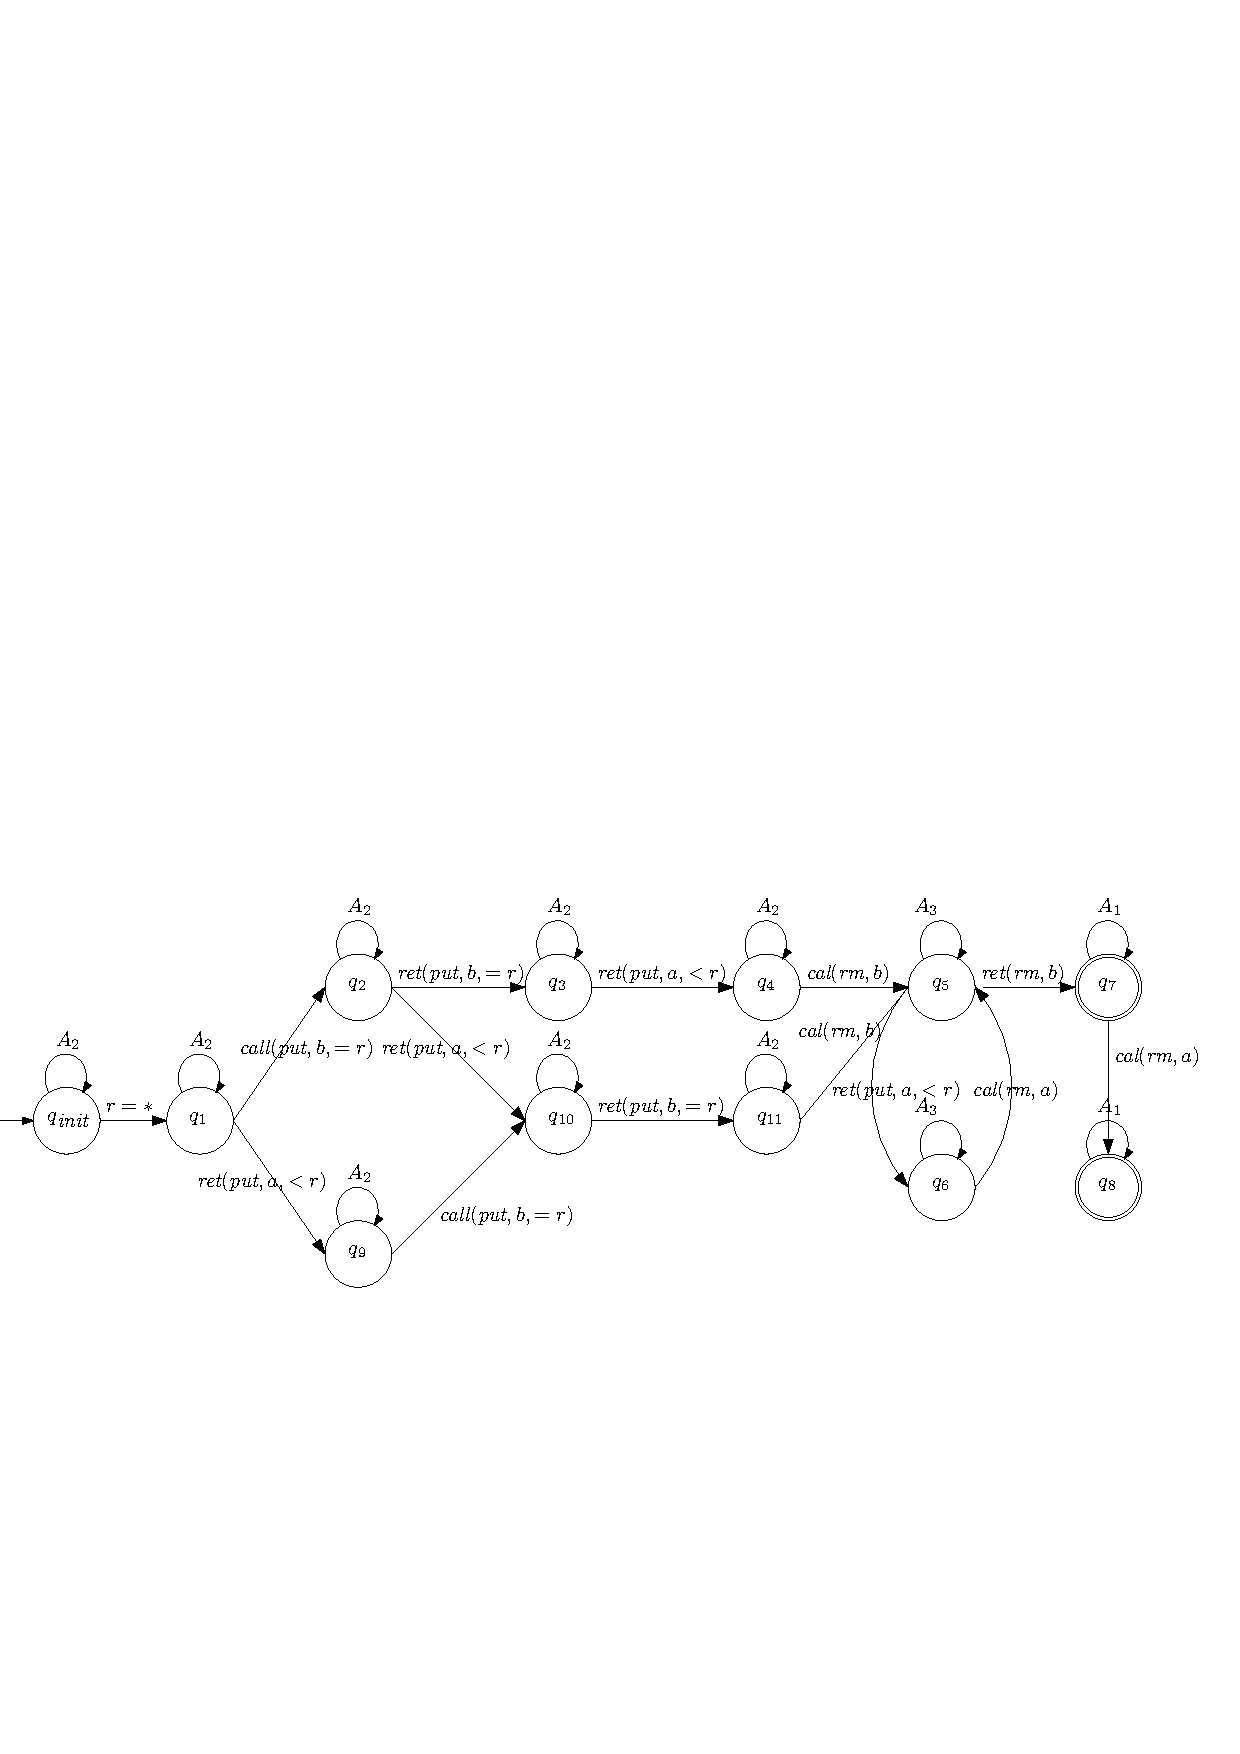
\includegraphics[width=1 \textwidth]{figures/PIC_AUTO_PQ1Lar-pprr.pdf}
%\vspace{-10pt}
  \caption{Automaton $\mathcal{A}_{\textit{l-lar}}^1$}
  \label{fig:automata APQ1Lar-1}
\end{figure}

$\mathcal{A}_{\textit{l-lar}}^1$ is used to recognize conditions in \figurename~\ref{fig:his for APQ1Lar-1}. Here for simplicity, we only draw operation of $b$, and the first $\textit{ret}(\textit{put},a,\_)$.


\begin{figure}[htbp]
  \centering
  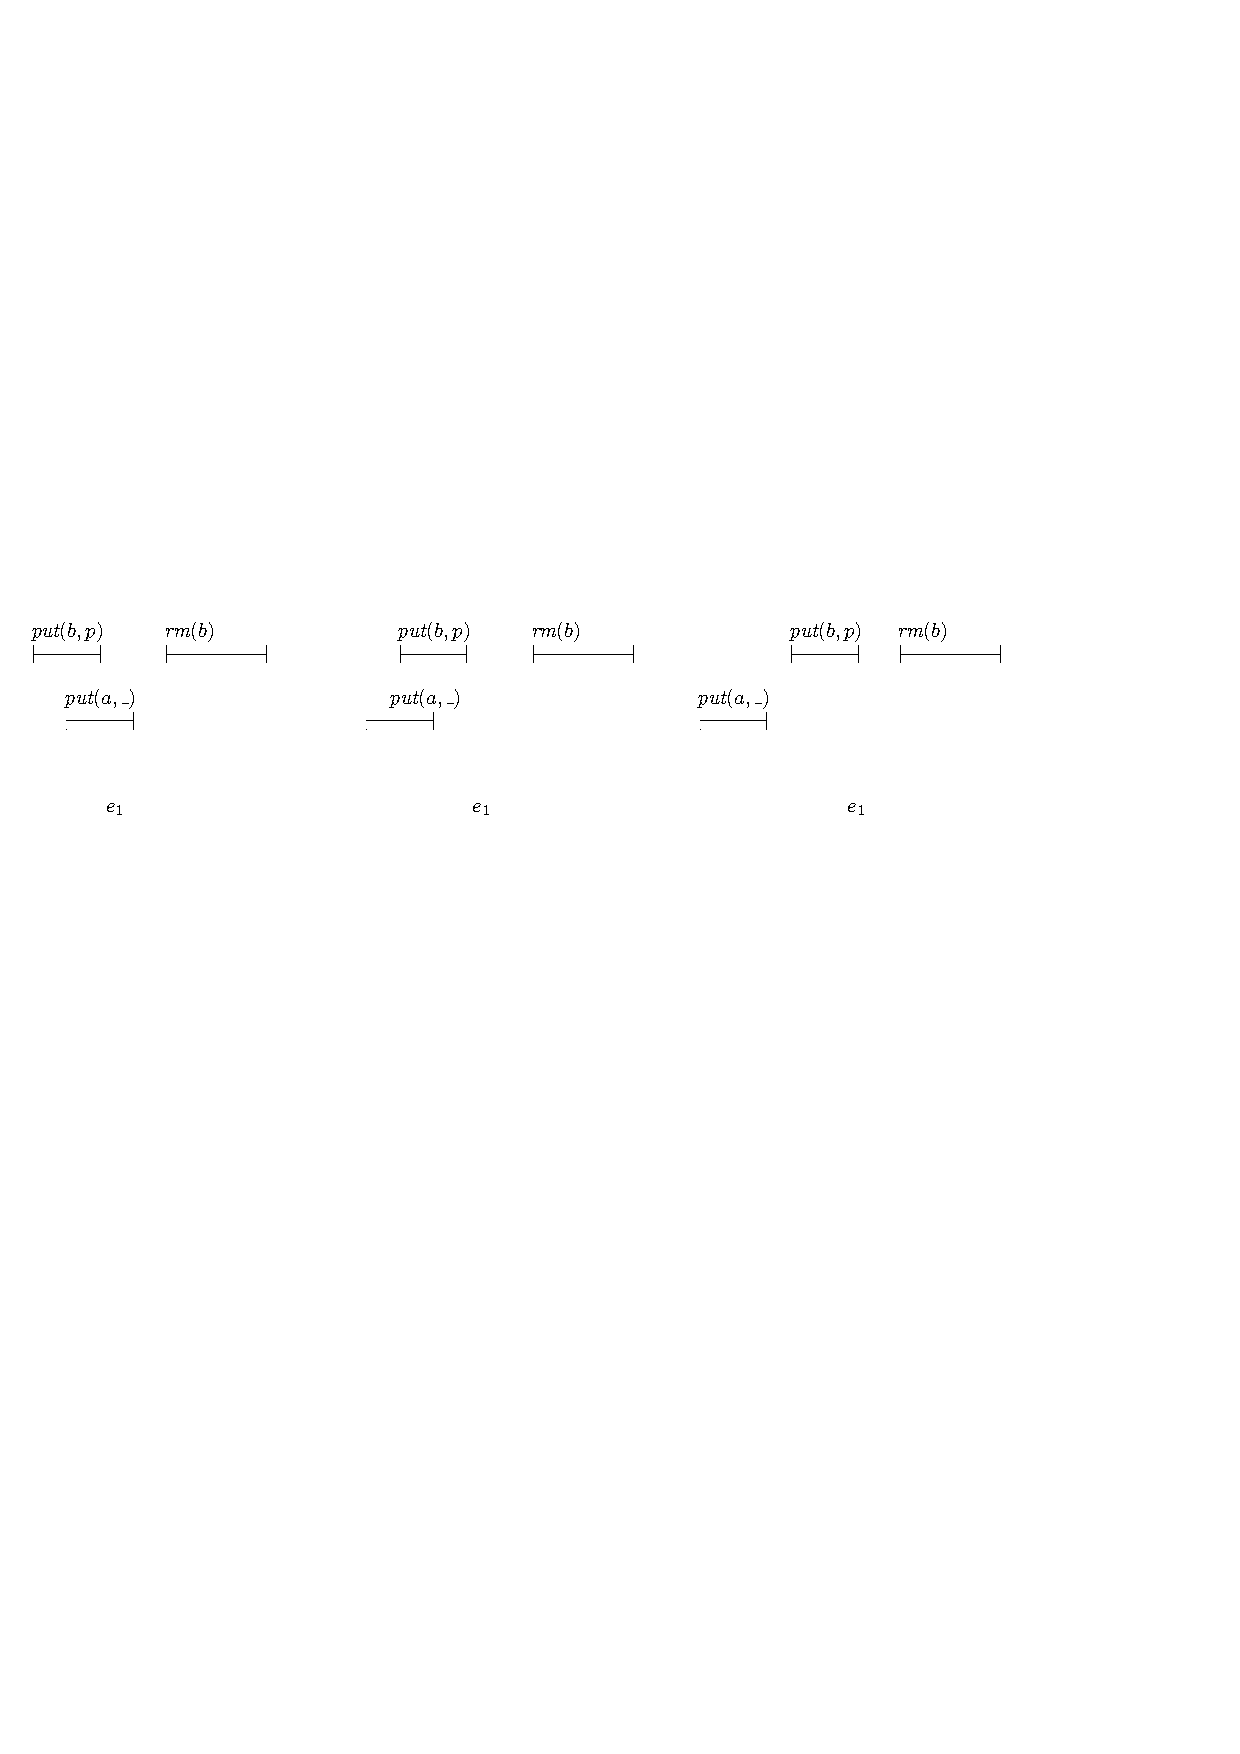
\includegraphics[width=1 \textwidth]{figures/PIC_HIS_PQ1Lar-pprr.pdf}
%\vspace{-10pt}
  \caption{Conditions recognized by $\mathcal{A}_{\textit{l-lar}}^1$}
  \label{fig:his for APQ1Lar-1}
\end{figure}


For the case when $e_r \vert_{b} = \textit{call}(\textit{put},b,p) \cdot \textit{call}(\textit{rm},b) \cdot \textit{ret}(\textit{put},b,p) \cdot \textit{ret}(\textit{rm},b)$, we generate register automaton $\mathcal{A}_{\textit{l-lar}}^2$, as shown in \figurename~\ref{fig:automata APQ1Lar-2}. Here $C_1,C_2,C_3$ is the same as that in $\mathcal{A}_{\textit{l-lar}}^1$. The differentiated branch in $\mathcal{A}_{\textit{l-lar}}^2$ comes from the positions of the first $\textit{ret}(\textit{put},a,\_)$.

\begin{figure}[htbp]
  \centering
  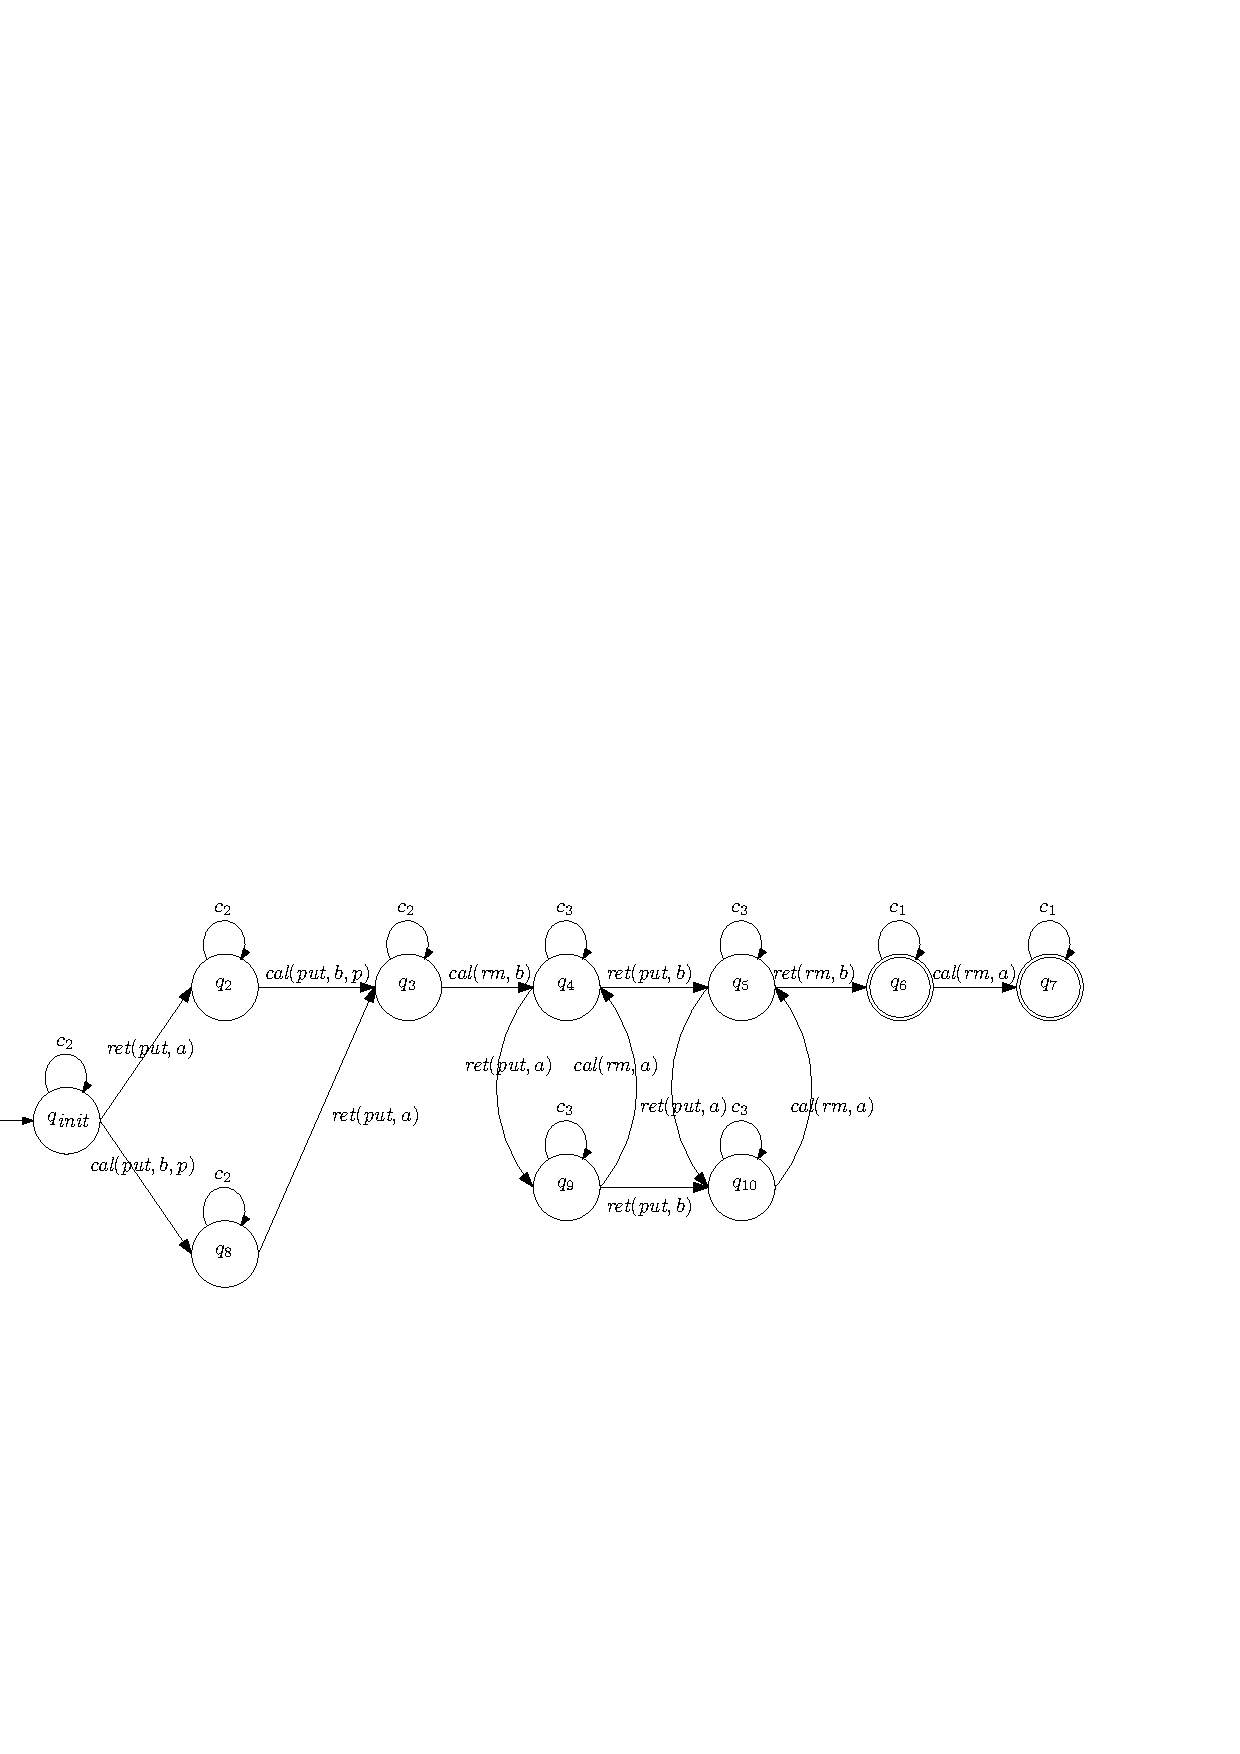
\includegraphics[width=1 \textwidth]{figures/PIC_AUTO_PQ1Lar-prpr.pdf}
%\vspace{-10pt}
  \caption{Automaton $\mathcal{A}_{\textit{l-lar}}^2$}
  \label{fig:automata APQ1Lar-2}
\end{figure}


$\mathcal{A}_{\textit{l-lar}}^2$ is used to recognize conditions in \figurename~\ref{fig:his for APQ1Lar-2}. Here for simplicity, we only draw operation of $b$, and the first $\textit{ret}(\textit{put},a,\_)$.


\begin{figure}[htbp]
  \centering
  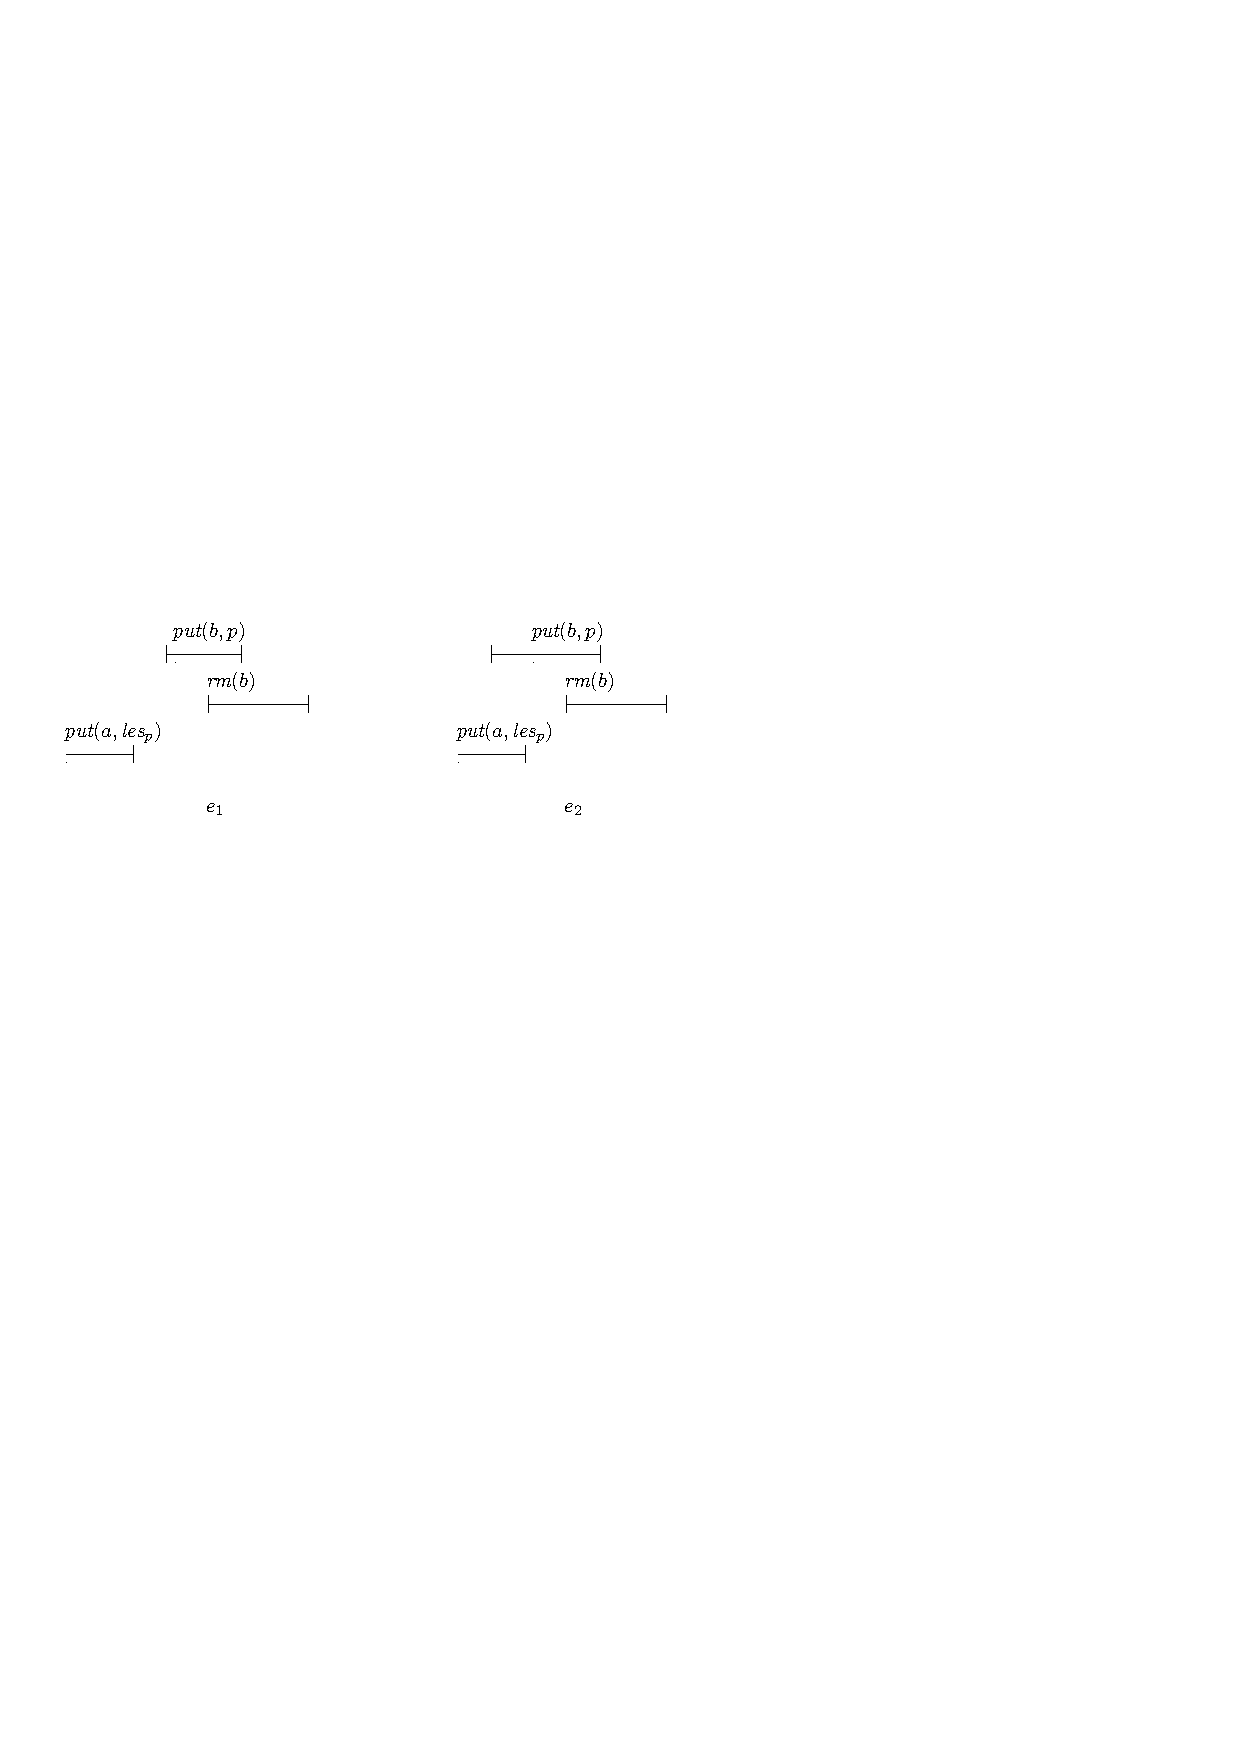
\includegraphics[width=0.7 \textwidth]{figures/PIC_HIS_PQ1Lar-prpr.pdf}
%\vspace{-10pt}
  \caption{Conditions recognized by $\mathcal{A}_{\textit{l-lar}}^2$}
  \label{fig:his for APQ1Lar-2}
\end{figure}

For the case when $e_r \vert_{b} = \textit{call}(\textit{rm},b) \cdot \textit{call}(\textit{put},b,p) \cdot \textit{ret}(\textit{put},b,p) \cdot \textit{ret}(\textit{rm},b)$, we generate register automaton $\mathcal{A}_{\textit{l-lar}}^3$, as shown in \figurename~\ref{fig:automata APQ1Lar-3}. Here $C_1,C_2,C_3$ is the same as that in $\mathcal{A}_{\textit{l-lar}}^1$. The differentiated branch in $\mathcal{A}_{\textit{l-lar}}^3$ comes from the positions of the first $\textit{ret}(\textit{put},a,\_)$.

\begin{figure}[htbp]
  \centering
  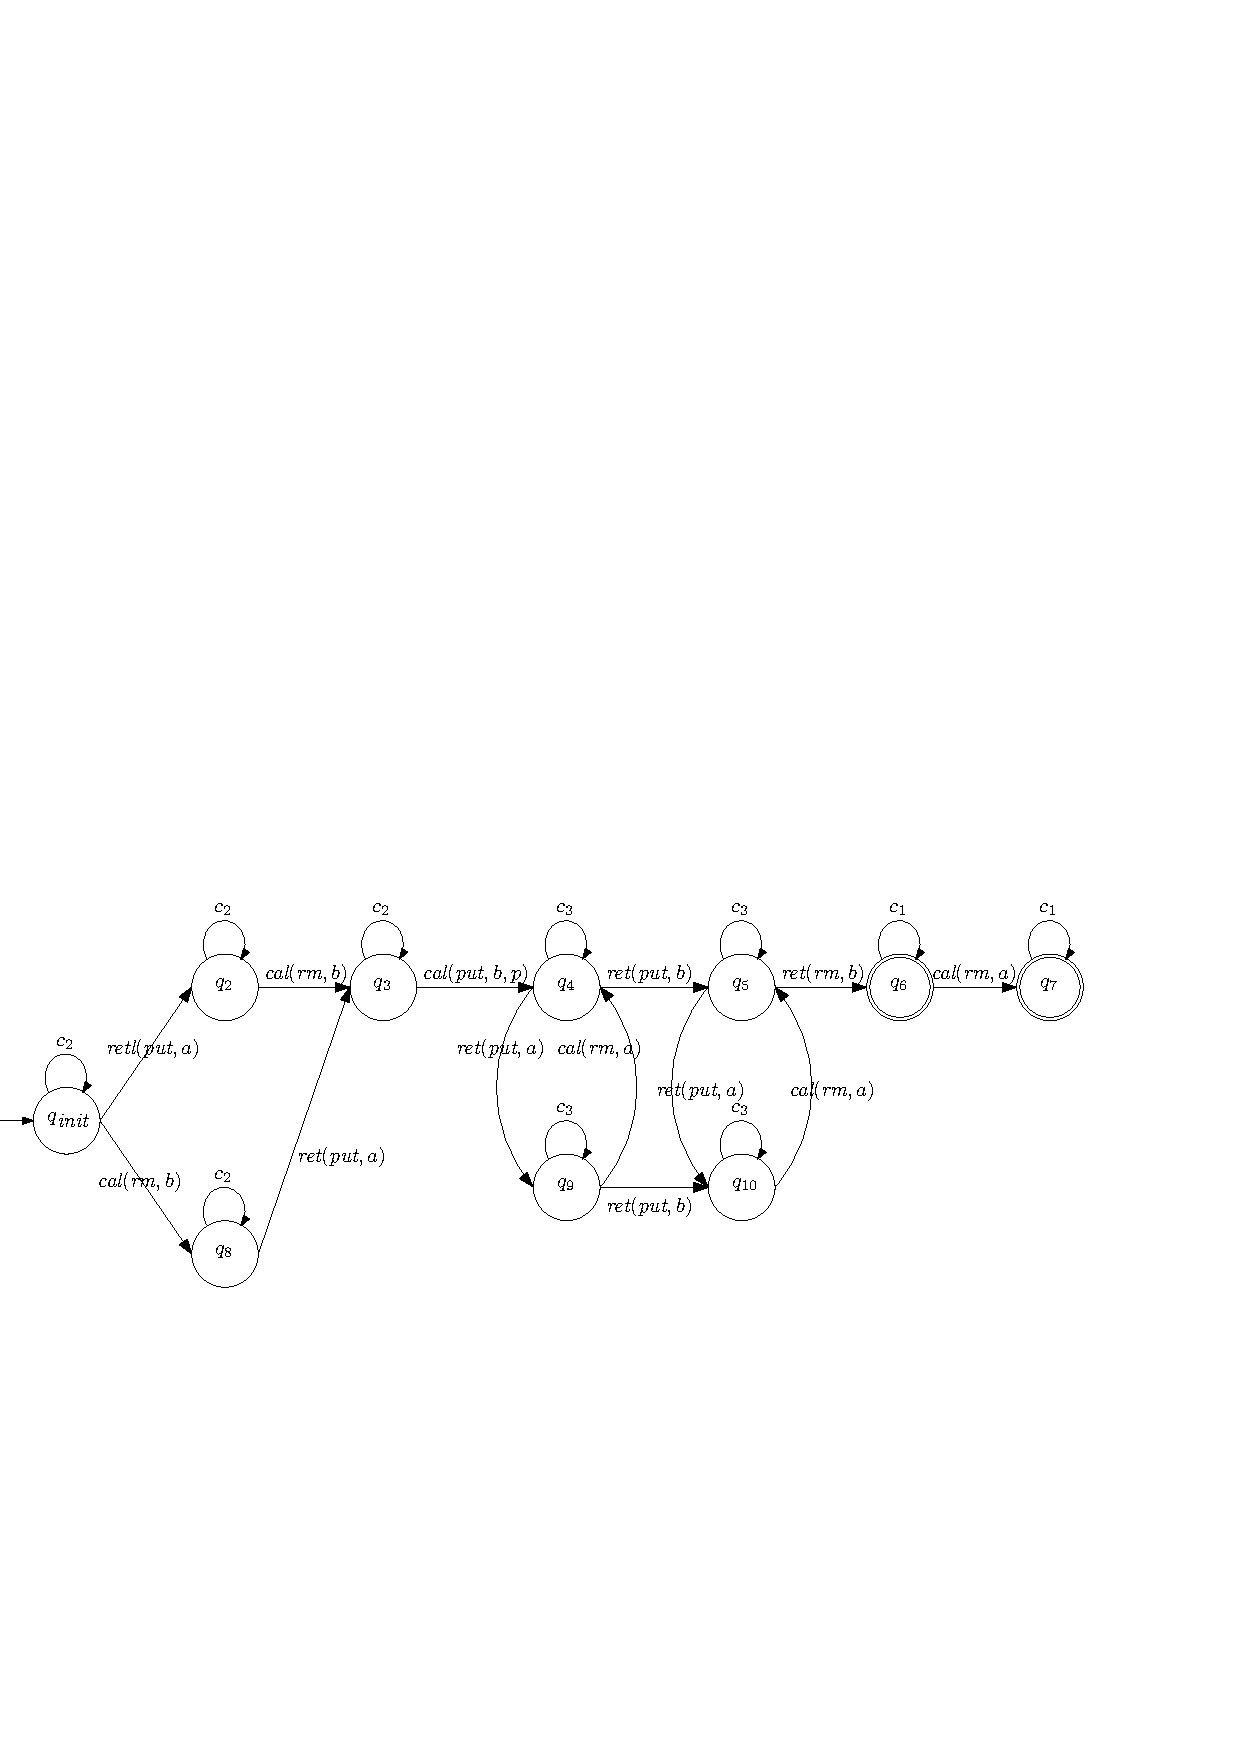
\includegraphics[width=1 \textwidth]{figures/PIC_AUTO_PQ1Lar-rppr.pdf}
%\vspace{-10pt}
  \caption{Automaton $\mathcal{A}_{\textit{l-lar}}^3$}
  \label{fig:automata APQ1Lar-3}
\end{figure}


$\mathcal{A}_{\textit{l-lar}}^3$ is used to recognize conditions in \figurename~\ref{fig:his for APQ1Lar-3}. Here for simplicity, we only draw operation of $b$, and the first $\textit{ret}(\textit{put},a,\_)$.


\begin{figure}[htbp]
  \centering
  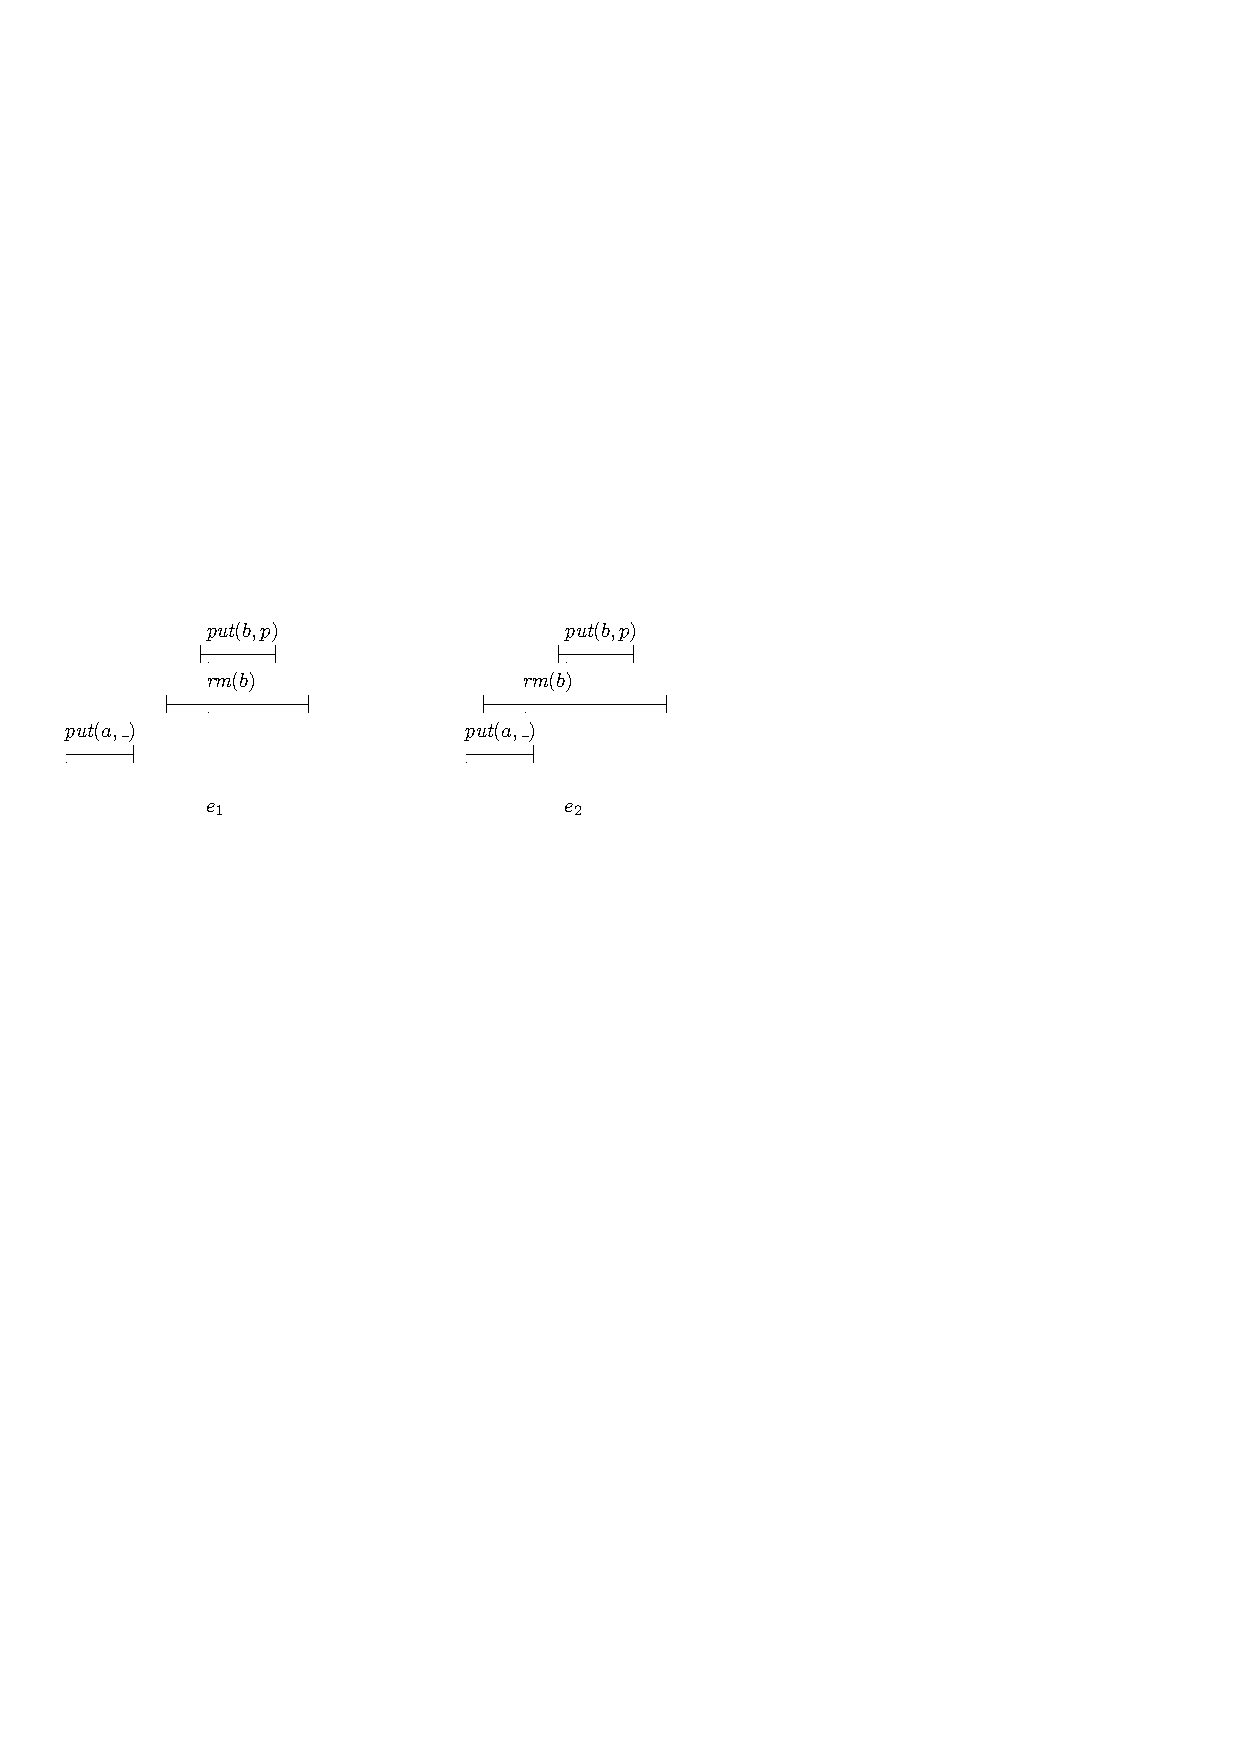
\includegraphics[width=0.7 \textwidth]{figures/PIC_HIS_PQ1Lar-rppr.pdf}
%\vspace{-10pt}
  \caption{Conditions recognized by $\mathcal{A}_{\textit{l-lar}}^3$}
  \label{fig:his for APQ1Lar-3}
\end{figure}


For the case when $e_r \vert_{b} = \textit{call}(\textit{rm},b) \cdot \textit{call}(\textit{put},b,p) \cdot \textit{ret}(\textit{rm},b) \cdot \textit{ret}(\textit{put},b,p)$, we generate register automaton $\mathcal{A}_{\textit{l-lar}}^4$, as shown in \figurename~\ref{fig:automata APQ1Lar-4}. Here $C_1,C_2,C_3$ is the same as that in $\mathcal{A}_{\textit{l-lar}}^1$, and $C_4 = C_1 \cup \{ \textit{ret}(\textit{put},b,=r) \}$. The differentiated branch in $\mathcal{A}_{\textit{l-lar}}^4$ comes from the positions of the first $\textit{ret}(\textit{put},a,\_)$.

\begin{figure}[htbp]
  \centering
  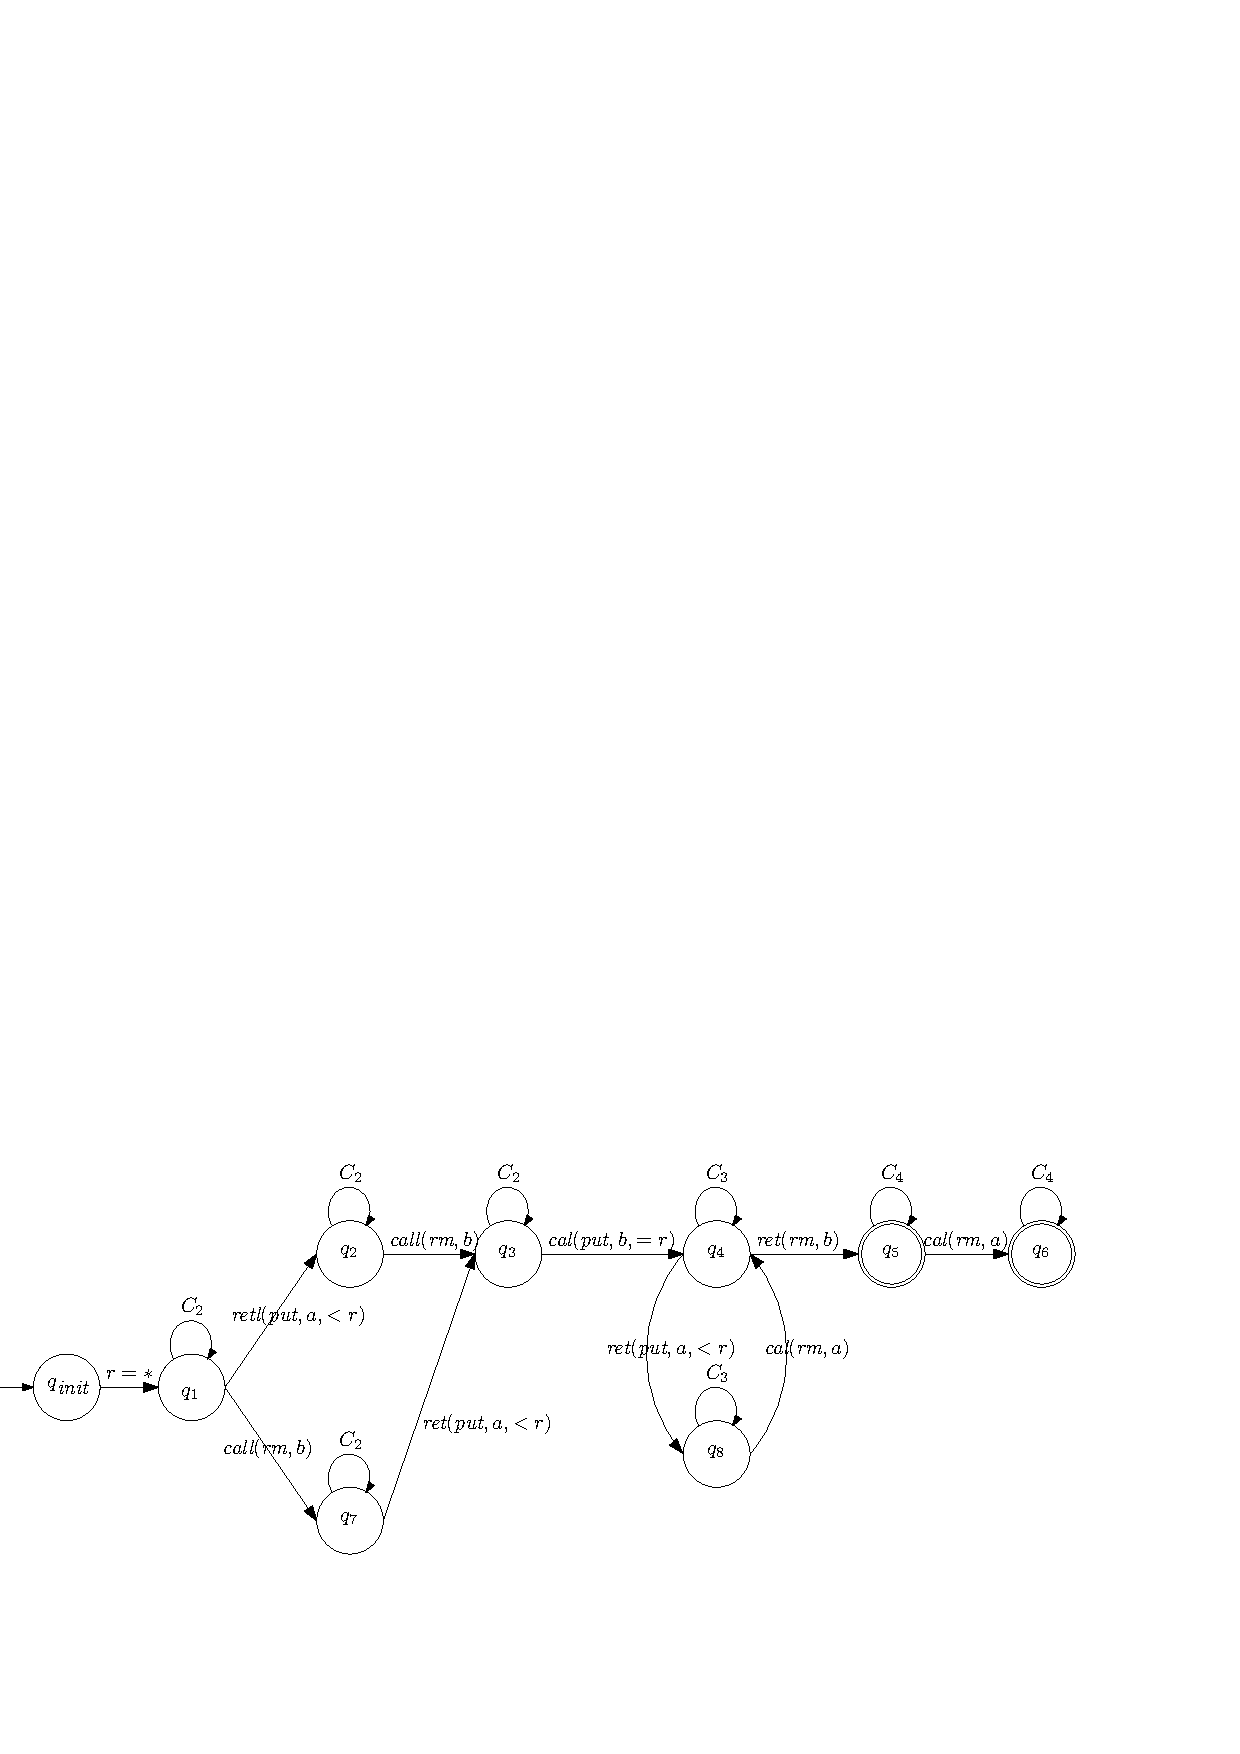
\includegraphics[width=0.9 \textwidth]{figures/PIC_AUTO_PQ1Lar-rprp.pdf}
%\vspace{-10pt}
  \caption{Automaton $\mathcal{A}_{\textit{l-lar}}^4$}
  \label{fig:automata APQ1Lar-4}
\end{figure}


$\mathcal{A}_{\textit{l-lar}}^4$ is used to recognize conditions in \figurename~\ref{fig:his for APQ1Lar-4}. Here for simplicity, we only draw operation of $b$, and the first $\textit{ret}(\textit{put},a,\_)$.


\begin{figure}[htbp]
  \centering
  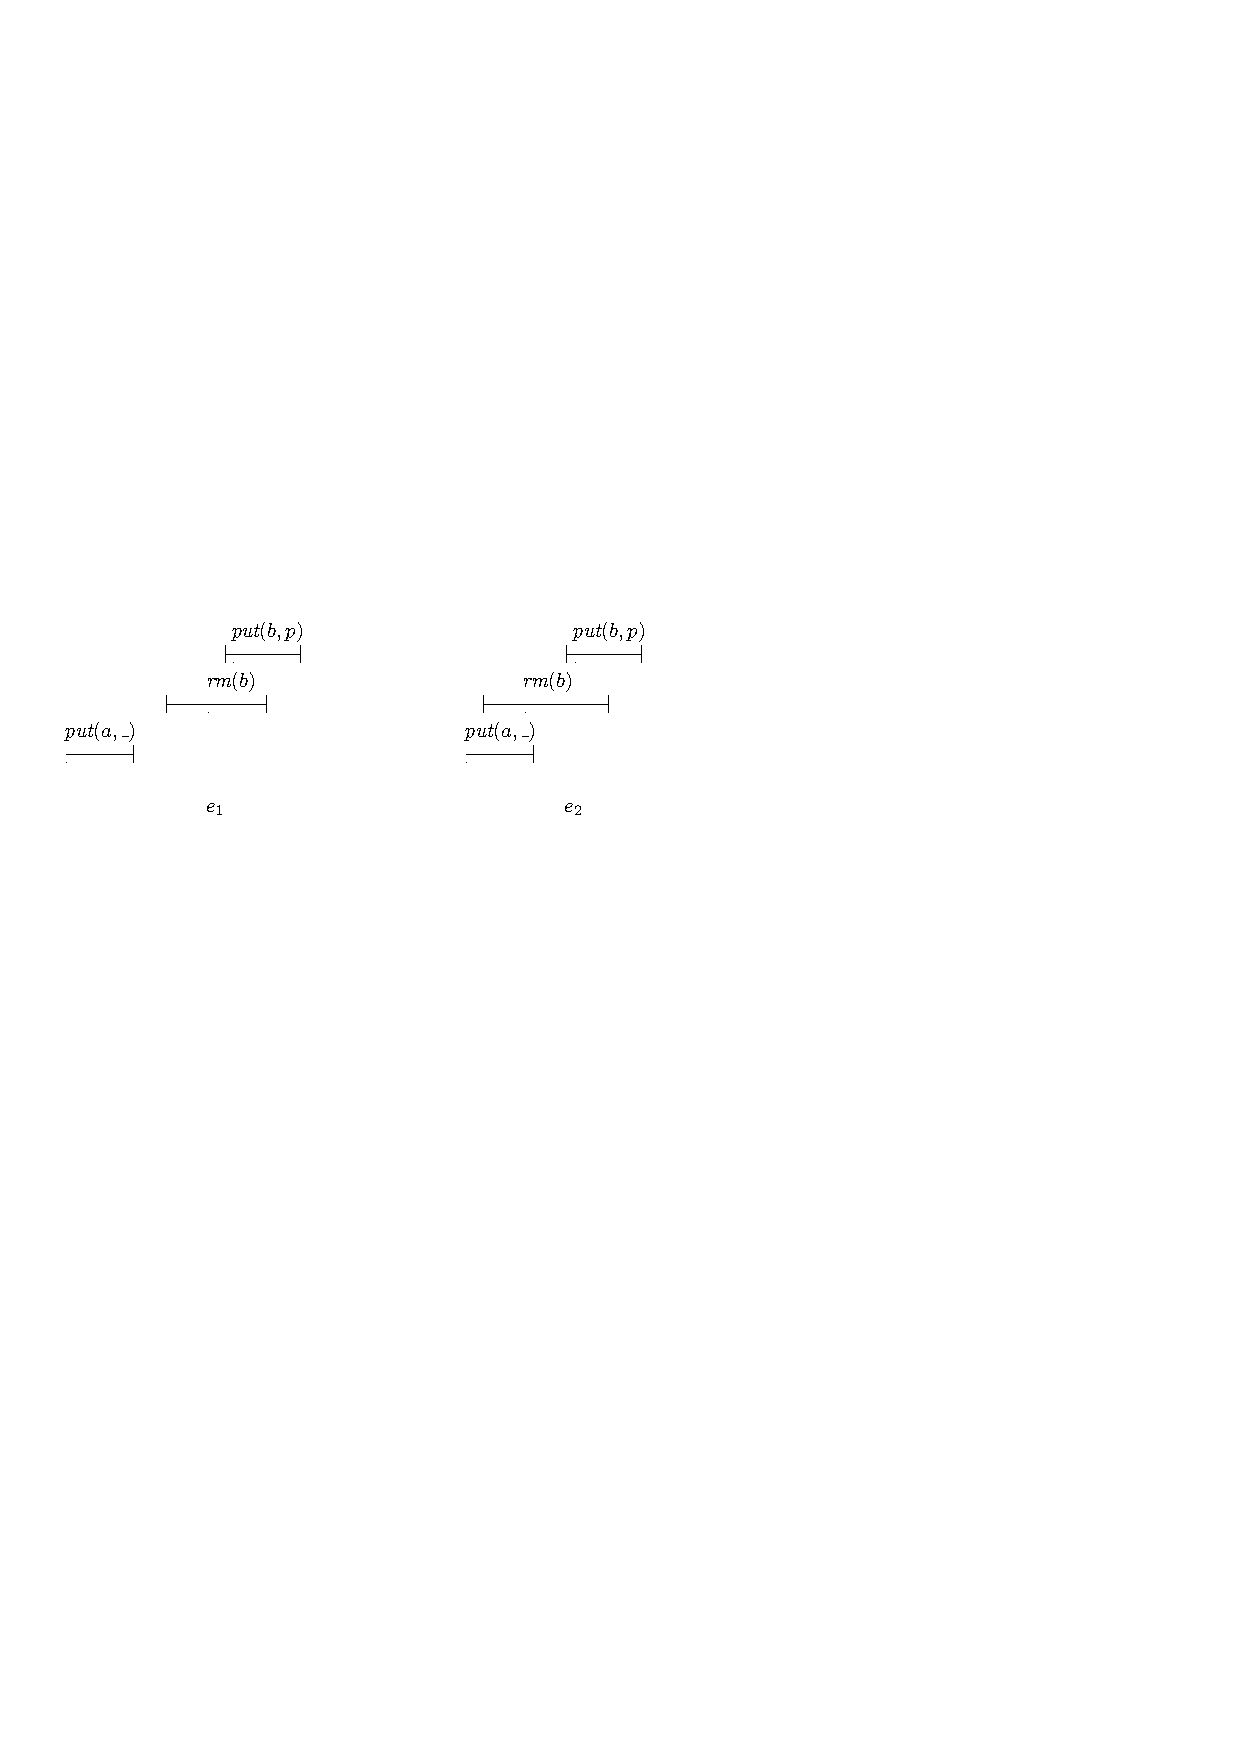
\includegraphics[width=0.7 \textwidth]{figures/PIC_HIS_PQ1Lar-rprp.pdf}
%\vspace{-10pt}
  \caption{Conditions recognized by $\mathcal{A}_{\textit{l-lar}}^4$}
  \label{fig:his for APQ1Lar-4}
\end{figure}

Let $\mathcal{A}_{\textit{1-lar}}$ be the union of $\mathcal{A}_{\textit{l-lar}}^1, \mathcal{A}_{\textit{l-lar}}^2, \mathcal{A}_{\textit{l-lar}}^3$ and $\mathcal{A}_{\textit{l-lar}}^4$. The following lemma states that $\mathcal{A}_{\textit{1-lar}}$ is $\mathsf{MatchedMaxPriority}^{>}$-complete. 


%\EPQOneLarisCoRegular*
\begin{restatable}{lemma}{EPQOneLarisCoRegular}
\label{lemma:EPQ1Lar is co-regular}
$\mathcal{A}_{\textit{1-lar}}$ is $\mathsf{MatchedMaxPriority}^{>}$-complete.
\end{restatable}


\begin {proof} 

We need to prove that, given a data-independent implementation $\mathcal{I}$. $\mathcal{A}_{\textit{1-lar}} \cap \mathcal{I} \neq \emptyset$ if and only if there exists $e \in \mathcal{I}$ and $e' \in \textit{proj}(e)$ such that $e'$ is not $\mathsf{MatchedMaxPriority}^{>}$-linearizable. 

By Lemma \ref{lemma:pri execution is enough} and Lemma \ref{lemma:Lin Equals Constraint for EPQ1Lar}, we need to prove the following fact:

\noindent {\bf $\textit{fact}_1$}: Given a data-independent implementation $\mathcal{I}$. $\mathcal{A}_{\textit{1-lar}} \cap \mathcal{I} \neq \emptyset$ if and only if there exists $e \in \mathcal{I}$ and $e' \in \textit{proj}(e)$, $\mathsf{Has\text{-}MatchedMaxPriority}(e)$ holds, $x$ is the value with maximal priority in $e'$, $e'$ has only one maximal priority, and there is a cycle going through $x$ in $G$, where $G$ is the left-right constraint of $x$ in $e'$. 

\noindent The $\textit{only if}$ direction: Let us consider the case of $\mathcal{A}_{\textit{l-lar}}^1$. Assume that $e_1 \in \mathcal{I}$ is accepted by $\mathcal{A}_{\textit{l-lar}}^1$. By data-independence, there exists data-differentiated execution $e \in \mathcal{I}$ and renaming function $r_1$, such that $e_1 = r_1(e)$. Assume that $r_1$ maps $d$ into $b$ and maps $f_1,\ldots,f_m$ into $a$. Let $e'$ be obtained from $e$ by projection into $\{ d, f_1,\ldots,f_m \}$. Assume that the priority of $b$ is $p$. It is easy to see that $e'$ has only one maximal priority, $\mathsf{Has\text{-}MatchedMaxPriority}(e')$ holds, and there is a cycle going through $d$ in $G$, where $G$ is the left-right constraint of $e'$. The case of $\mathcal{A}_{\textit{l-lar}}^2$, $\mathcal{A}_{\textit{l-lar}}^3$ and $\mathcal{A}_{\textit{l-lar}}^4$ can be similarly proved.

\noindent The $\textit{if}$ direction: Given such $e$, $e'$ and $x$. Let renaming function $r$ maps $x$ into $b$, maps items cover $x$ into $a$, and maps other items into $d$. By data-independence, $r(e) \in \mathcal{I}$. Then depending on the cases of $r(e) \vert_{b}$, we can see that $r(e)$ is accepted by $\mathcal{A}_{\textit{l-lar}}^1$, $\mathcal{A}_{\textit{l-lar}}^2$, $\mathcal{A}_{\textit{l-lar}}^3$ or $\mathcal{A}_{\textit{l-lar}}^4$. \qed
\end {proof}



\subsection{Proofs, Definitions and Register Automata in Subsection \ref{subsec:co-regular of EPQ1Equal}}
\label{sec:appendix proof and definition in section co-regular of EPQ1Equal}

Let $\textit{Items}(e,p)$ be the set of items with priority $p$ in execution $e$. The following lemma states a method to build the linearization of $e$ w.r.t $\mathsf{MatchedMaxPriority}^{=}$. 

\begin{restatable}{lemma}{MaximalInPBadGPMakePQ1Equal}
\label{lemma:maximal in pb and gap-point make a candidate of EPQ1Equal}
Given a data-differentiated execution $e$ where $\mathsf{Has\text{-}MatchedMaxPriority}^{=}(e)$ holds and $p$ is its maximal priority. If there exists a value $x$ with priority $p$, such that for each $y \in \textit{Items}(e,p)$, (1) $x\not<_{\textit{pb}}y$, and (2) the right-most gap-point of $x$ is after $\textit{call}(\textit{put},y,p)$ and $\textit{call}(\textit{rm},y)$. Then $e$ is $\mathsf{MatchedMaxPriority}^{=}$-linearizable. 
\end{restatable}

\begin {proof}

Let $o$ be the right-most gap-point of $x$. We locate linearization points of each operation as follows:

\begin{itemize}
\setlength{\itemsep}{0.5pt}
\item[-] Locate the linearization point of $\textit{rm}(x)$ at $o$,

\item[-] If $\textit{put}(x,p)$ overlaps with $\textit{rm}(x)$, then locate the linearization point of $\textit{put}(x,p)$ just before the linearization point of $\textit{rm}(x)$. Otherwise, $\textit{put}(x,p) <_{\textit{hb}} \textit{rm}(x)$, and we locate the linearization point of $\textit{put}(x,p)$ just before its return action.

\item[-] Locate linearization points of operation of each $y \in \textit{Items}(e,p)$ (except for $x$) just after the call action of the operation.

\item[-] For item $z$ with priority smaller than $p$. If both $\textit{call}(\textit{put},z,\_)$ and $\textit{call}(\textit{rm},z)$ is before $o$, then locate the linearization points of $\textit{put}(z,\_)$ and $\textit{rm}(z)$ just after their call actions. If both $\textit{ret}(\textit{put},z)$ and $\textit{ret}(\textit{rm},z)$ (if exists) is after $o$, then locate the linearization points of $\textit{put}(z,\_)$ and $\textit{rm}(z)$ just before their return actions. Otherwise, $x$ is in interval of $z$, which contradicts the definition of gap-point, and is impossible.
\end{itemize}

Let $l$ be the sequence of linearization points constructed above. It is obvious that $e \sqsubseteq l$. Since for each $y \in \textit{Items}(e,p)$, $o$ is after $\textit{call}(\textit{put},y,\_)$ and $\textit{call}(\textit{rm},x)$, we can see that $\textit{rm}(x)$ is after $\textit{put}(y,p)$ and $\textit{rm}(y)$ in $l$. It is obvious that $\textit{put}(x,p)$ is before $\textit{rm}(x)$ in $l$. Since $x$ does not $<_{\textit{pb}}$ to $y$, we can see that no $\textit{put}(y,p)$ happens before $\textit{put}(x,p)$. Then it is easy to see that $\textit{put}(x,p)$ is after $\textit{put}(y,p)$ in $l$. Since $\mathsf{Has\text{-}MatchedMaxPriority}^{=}(e)$ holds, all other items in $\textit{Items}(e,p)$ has matched $\textit{put}$ and $\textit{rm}$, and it is easy to see that their $\textit{put}$ and $\textit{rm}$ (except for that of $x$) are all before $\textit{rm}(x)$ in $l$.

For item $z$ with priority smaller than $p$, we can see that there are only two possibilities: (1) $\textit{put}(z,\_)$ and $\textit{rm}(z)$ are both before $\textit{rm}(x)$ in $l$, and (2) $\textit{put}(z,\_)$ and $\textit{rm}(z)$ (if exists) are after before $\textit{rm}(x)$ in $l$. Therefore, before $\textit{rm}(x)$ in $l$, the $\textit{put}$ and $\textit{rm}$ of $z$ are matched.

Therefore, it is easy to see that $\mathsf{MatchedMaxPriority^{=}\text{-}Seq}(l,x)$ holds and $e$ is $\mathsf{MatchedMaxPriority}^{=}$-linearizable. \qed 
\end {proof}

With Lemma \ref{lemma:maximal in pb and gap-point make a candidate of EPQ1Equal}, we can prove the following lemma, which states that getting rid of case in \figurename~\ref{fig:introduce pb order} is enough for ensure that $\mathsf{MatchedMaxPriority}^{=}(e)$ holds. 


\EPQOneEqualAsPBandGP*

\begin {proof}

To prove the $\textit{if}$ direction, let $e_{x,y}$ be the execution that is obtained from $e$ by erasing all actions of items that has same priority as $x$, except for actions of $x$ and $y$. It is obvious that $\textit{last}(e_{x,y}) = \seqPQ_1^{=}$. Since $y <_{\textit{pb}}^* x$, according to $\seqPQ_1^{=}$, we can see that $x$ should be chosen as $\textit{itm}$ in $\seqPQ_1^{=}$.

According to Lemma \ref{lemma:Lin Equals Constraint for EPQ1Lar} (Here we temporarily forget the existence of $y$), the only possible position for locating linearizaton point of $\textit{rm}(x)$ is at gap-point of $x$. Otherwise, if the linearizaton point of $\textit{rm}(x)$ is chosen at a position that is not a gap-point of $x$, then there exists unmatched operation before $\textit{rm}(x)$ with smaller priority. Since the rightmost gap-point of $x$ is before $\textit{call}(\textit{put},y,p)$ or $\textit{call}(\textit{rm},y)$, if we locate linearizaton point of $\textit{rm}(x)$ at gap-point of $x$, then $\textit{rm}(x)$ will be before $\textit{call}(\textit{put},y,p)$ or $\textit{call}(\textit{rm},x)$.

Therefore, for every sequence $l = u \cdot \textit{put}(x,p) \cdot v \cdot \textit{rm}(x) \cdot w$, if $e_{x,y} \sqsubseteq l$, then either $u \cdot v$ contains some unmatched operations of priority smaller than $p$, or $w$ contains $\textit{put}(y,p)$ or $\textit{rm}(y)$. In both cases, $l \notin \textit{MS}(\seqPQ_1^{=})$.

To prove the $\textit{only if}$ direction, we prove its contrapositive. Assume we already know that for each $x$ and $y$ has maximal priority in $e$, if $y <_{\textit{pb}}^* x$, then the rightmost gap-point of $x$ is after $\textit{call}(\textit{put},y,p)$ and $\textit{call}(\textit{rm},x)$. We need to prove that $e \sqsubseteq \textit{MS}(\seqPQ_1^{=})$. Recall that we already assume that each single-priority execution has FIFO property, and item with larger priority is not covered by items with smaller priority.

Our proof proceed as follows:

\begin{itemize}
\setlength{\itemsep}{0.5pt}
\item[-] Let $e_{p}$ be the projection of $e$ into operations of priority $p$. Since each single-priority execution has FIFO property, there exists sequence $l_{p}$, such that $e_{p} \sqsubseteq l_{p}$, and when we treat $\textit{put}$ as $\textit{enq}$ and $\textit{rm}$ as $\textit{deq}$, $l_{p}$ belongs to queue.

\item[-] Let $a_1$ be the last inserted item of $l_{p}$.

    Step $1$: Check whether for each $b \in \textit{Items}(e,p)$, (1) $a_1$ does not $<_{\textit{pb}}$ to $b$, and (2) the right-most gap-point of $a$ is after $\textit{call}(\textit{put},b,p)$ and $\textit{call}(\textit{rm},b)$.

    It is easy to see that $a_1$ is of priority $p$, and $a_1$ does not $<_{\textit{pb}}$ to any $b \in \textit{Items}(e,p)$. If for each $b \in \textit{Items}(e,p)$, the rightmost gap-point of $a_1$ is after $\textit{call}(\textit{put},b,p)$ and $\textit{call}(\textit{rm},b)$. Then by Lemma \ref{lemma:maximal in pb and gap-point make a candidate of EPQ1Equal}, we can obtain that $e \sqsubseteq \textit{MS}(\seqPQ_1^{=})$.


\item[-] Otherwise, there exists $a_2 \in \textit{Items}(e,p)$, such that the rightmost gap-point of $a_1$ is before $\textit{call}(\textit{put},a_2,p)$ or $\textit{call}(\textit{rm},a_2)$ in $e$. We can see that each gap-point of $a_2$ is after the rightmost gap-point of $a_1$.%, and thus, the right-most gap-point of $a_2$ is after the rightmost gap-point of $a_1$.
    By assumption, we know that $a_2$ does not $<_{\textit{pb}}$ to $a_1$.

    \begin{itemize}
    \setlength{\itemsep}{0.5pt}
    \item[-] If for each item $b \in \textit{Items}(e,p)$, $a_2$ does not $<_{\textit{pb}}$ to $b$. Then we go to step $1$ and treat $a_2$ similarly as $a_1$.
    \item[-] Otherwise, there exists $a_3$ with priority $p$ such that $a_2 <_{\textit{pb}}^* a_3$.

    Since $l_{p}$ has FIFO property, it is easy to see that there is no cycle in $<_{\textit{pb}}$ order. It is safe to assume that $a_3$ is maximal in the sense of $<_{\textit{pb}}^*$. Or we can say, there does not exists $a_4$, such that $a_3 <_{\textit{pb}}^* a_4$.

    By assumption,we know that the rightmost gap-point of $a_3$ is after $\textit{call}(\textit{put},a_2,p)$ and $\textit{call}(\textit{rm},a_2)$. Therefore, we can see that the rightmost gap-point of $a_3$ is after the rightmost gap-point of $a_1$. Then we go to step $1$ and treat $a_3$ similarly as $a_1$.
    \end{itemize}
\end{itemize}

Let $a^i$ be the $a_1$ in the $\textit{i-th}$ loop of our proof. It is not hard to see that, given $i<j$, the rightmost gap-point of $a^j$ is after the rightmost gap-point of $a^i$. Therefore, the loop finally stop at some $a^f$. $a^f$ satisfies the check of Step $1$. By Lemma \ref{lemma:maximal in pb and gap-point make a candidate of EPQ1Equal}, this implies that $e \sqsubseteq \textit{MS}(\seqPQ_1^{=})$. This completes the proof of $\textit{if}$ direction. \qed
\end {proof}



According to the definition of $<_{\textit{ob}}^*$, if $a <_{\textit{pb}}^* b$, then there exists $a_1,\ldots,a_m$, such that $a <_{\textit{pb}} a_1 <_{\textit{pb}} \ldots <_{\textit{pb}} a_m <_{\textit{pb}} b$. The following lemma states that, the number of intermediate items $a_i$ is in fact bounded.

\OBOrderHasBoundedLength*

\begin {proof}

Our proof proceed as follows:

\begin{itemize}
\setlength{\itemsep}{0.5pt}
\item[-] ($<_{\textit{pb}}^A \cdot <_{\textit{pb}}^A$,$<_{\textit{pb}}^B \cdot <_{\textit{pb}}^B$ and $<_{\textit{pb}}^C \cdot <_{\textit{pb}}^C$): If $c_3 <_{\textit{pb}}^A c_2 <_{\textit{pb}}^A c_1$, then $\textit{put}(c_3,\_)$ happens before $\textit{put}(c_2,\_)$, and $\textit{put}(c_2,\_)$ happens before $\textit{put}(c_1,\_)$. Therefore, it is obvious that $\textit{put}(c_3,\_)$ happens before $\textit{put}(c_1,\_)$ and $c_3 <_{\textit{pb}}^A c_1$.

    Similarly, if $c_3 <_{\textit{pb}}^B c_2 <_{\textit{pb}}^B c_1$, then $c_3 <_{\textit{pb}}^B c_1$.

    If $c_3 <_{\textit{pb}}^C c_2 <_{\textit{pb}}^C c_1$: Since $c_2 <_{\textit{pb}}^C c_1$, $\textit{ret}(\textit{rm},c_2)$ is before $\textit{call}(\textit{put},c_1,\_)$. Since $\textit{rm}(c_2)$ does not happen before $\textit{put}(c_2,\_)$, $\textit{call}(\textit{put},c_2,\_)$ is before $\textit{ret}(\textit{rm},c_2)$. Since $c_3 <_{\textit{pb}}^C c_2$, $\textit{ret}(\textit{rm},c_3)$ is before $\textit{call}(\textit{put},c_2,\_)$. Therefore, $\textit{ret}(\textit{rm},c_3)$ is before $\textit{call}(\textit{put},c_1,\_)$, and $c_3 <_{\textit{pb}}^C c_1$.

    Therefore, when we meet successive $<_{\textit{pb}}^A$, it is safe to leave only the first and the last elements and ignore intermediate elements. Similar cases hold for $<_{\textit{pb}}^B$ and $<_{\textit{pb}}^C$.

\item[-] $<_{\textit{pb}}^A$ and $<_{\textit{pb}}^C$:

    \begin{itemize}
    \setlength{\itemsep}{0.5pt}
    \item[-] ($<_{\textit{pb}}^A \cdot <_{\textit{pb}}^C$): If $c_3 <_{\textit{pb}}^A c_2 <_{\textit{pb}}^C c_1$. Since $c_2 <_{\textit{pb}}^C c_1$, $\textit{ret}(\textit{rm},c_2)$ is before $\textit{call}(\textit{put},c_1,\_)$. Since $\textit{rm}(c_2)$ does not happen before $\textit{put}(c_2,\_)$, $\textit{call}(\textit{put},c_2,\_)$ is before $\textit{ret}(\textit{rm},c_2)$. Since $c_3 <_{\textit{pb}}^A c_2$, $\textit{ret}(\textit{put},c_3)$ is before $\textit{call}(\textit{put},c_2,\_)$. Therefore, $\textit{ret}(\textit{put},c_3)$ is before $\textit{call}(\textit{put},c_1,\_)$, and $c_3 <_{\textit{pb}}^A c_1$.

    \item[-] ($<_{\textit{pb}}^C \cdot <_{\textit{pb}}^A$): If $c_3 <_{\textit{pb}}^C c_2 <_{\textit{pb}}^A c_1$. Since $c_2 <_{\textit{pb}}^A c_1$, $\textit{ret}(\textit{put},c_2)$ is before $\textit{call}(\textit{put},c_1,\_)$. It is obvious that $\textit{call}(\textit{put},c_2,\_)$ is before $\textit{ret}(\textit{put},c_2)$. Since $c_3 <_{\textit{pb}}^C c_2$, $\textit{ret}(\textit{rm},c_3)$ is before $\textit{call}(\textit{put},c_2,\_)$. Therefore, $\textit{ret}(\textit{rm},c_3)$ is before $\textit{call}(\textit{put},c_1,\_)$, and $c_3 <_{\textit{pb}}^C c_1$.

    %Since $c_2 <_{\textit{pb}}^A c_1$, $\textit{put}(c_2,\_)$ happens before $\textit{put}(c_1,\_)$. Since $c_3 <_{\textit{pb}}^C c_2$, $\textit{rm}(c_3)$ happens before $\textit{put}(c_2,\_)$. Therefore, $\textit{rm}(c_3)$ happens before $\textit{put}(c_1,\_)$, and $c_3 <_{\textit{pb}}^C c_1$.
    \end{itemize}

\item[-] $<_{\textit{pb}}^B$ and $<_{\textit{pb}}^C$:

    \begin{itemize}
    \setlength{\itemsep}{0.5pt}
    \item[-] ($<_{\textit{pb}}^B \cdot <_{\textit{pb}}^C$): If $c_3 <_{\textit{pb}}^B c_2 <_{\textit{pb}}^C c_1$. Since $c_2 <_{\textit{pb}}^C c_1$, $\textit{ret}(\textit{rm},c_2)$ is before $\textit{call}(\textit{put},c_1,\_)$. It is obvious that $\textit{call}(\textit{rm},c_2)$ is before $\textit{ret}(\textit{rm},c_2)$. Since $c_3 <_{\textit{pb}}^B c_2$, $\textit{ret}(\textit{rm},c_3)$ is before $\textit{call}(\textit{rm},c_2)$. Therefore, $\textit{ret}(\textit{rm},c_3)$ is before $\textit{call}(\textit{put},c_1,\_)$, and $c_3 <_{\textit{pb}}^C c_1$.

    \item[-] ($<_{\textit{pb}}^C \cdot <_{\textit{pb}}^B$): If $c_3 <_{\textit{pb}}^C c_2 <_{\textit{pb}}^B c_1$. Since $c_2 <_{\textit{pb}}^B c_1$, $\textit{ret}(\textit{rm},c_2)$ is before $\textit{call}(\textit{rm},c_1)$. Since $\textit{rm}(c_2)$ does not happen before $\textit{put}(c_2,\_)$, $\textit{call}(\textit{put},c_2,\_)$ is before $\textit{ret}(\textit{rm},c_2)$. Since $c_3 <_{\textit{pb}}^C c_2$, $\textit{ret}(\textit{rm},c_3)$ is before $\textit{call}(\textit{put},c_2,\_)$. Therefore, $\textit{ret}(\textit{rm},c_3)$ is before $\textit{call}(\textit{rm},c_1)$, and $c_3 <_{\textit{pb}}^B c_1$.
    \end{itemize}

\item[-]  ($<_{\textit{pb}}^A \cdot <_{\textit{pb}}^B \cdot <_{\textit{pb}}^A$): If $c_4 <_{\textit{pb}}^A c_3 <_{\textit{pb}}^B c_2 <_{\textit{pb}}^A c_1$:
    \begin{itemize}
    \setlength{\itemsep}{0.5pt}
    \item[-] If $\textit{call}(\textit{rm},c_2)$ is before $\textit{call}(\textit{put},c_1,\_)$: Since $c_3 <_{\textit{pb}}^B c_2$, $\textit{ret}(\textit{rm},c_3)$ is before $\textit{call}(\textit{rm},c_2)$. Then $\textit{ret}(\textit{rm},c_3)$ is before $\textit{call}(\textit{put},c_1,\_)$, and $c_3 <_{\textit{pb}}^C c_1$. This implies that $c_4 <_{\textit{pb}}^A c_3 <_{\textit{pb}}^C c_1$. According to the fact for $<_{\textit{pb}}^A \cdot <_{\textit{pb}}^C$, we know that $c_4  <_{\textit{pb}}^A c_1$.

    \item[-] If $\textit{call}(\textit{rm},c_2)$ is after $\textit{call}(\textit{put},c_1,\_)$: Since $c_2 <_{\textit{pb}}^A c_1$, $\textit{ret}(\textit{put},c_2,\_)$ is before $\textit{call}(\textit{put},c_1,\_)$. Since $c_3 <_{\textit{pb}}^B c_2$, $\textit{rm}(c_3)$ happens before $\textit{rm}(c_2)$, and then we know that $\textit{put}(c_2,\_)$ can not happen before $\textit{put}(c_3,\_)$. Since $\textit{put}(c_2,\_)$ does not happen before $\textit{put}(c_3,\_)$, $\textit{call}(\textit{put},c_3,\_)$ is before $\textit{ret}(\textit{put},c_2,\_)$. Since $c_4 <_{\textit{pb}}^A c_3$, $\textit{ret}(\textit{put},c_4)$ is before $\textit{call}(\textit{put},c_3,\_)$. Therefore, $\textit{ret}(\textit{put},c_4)$ is before $\textit{call}(\textit{put},c_1,\_)$, and $c_4 <_{\textit{pb}}^A c_1$.
    \end{itemize}

\item[-]  ($<_{\textit{pb}}^B \cdot <_{\textit{pb}}^A \cdot <_{\textit{pb}}^B$): If $c_4 <_{\textit{pb}}^B c_3 <_{\textit{pb}}^A c_2 <_{\textit{pb}}^B c_1$: Since $c_2 <_{\textit{pb}}^B c_1$, $\textit{ret}(\textit{rm},c_2)$ is before $\textit{call}(\textit{rm},c_1)$. Since $c_3 <_{\textit{pb}}^A c_2$, we can see that $\textit{put}(c_3,\_) <_{\textit{hb}} \textit{put}(c_2,\_)$. Since each single-priority execution has FIFO property, we know that $\textit{rm}(c_2)$ does not happen before $\textit{rm}(c_3)$, and thus, $\textit{call}(\textit{rm},c_3)$ is before $\textit{ret}(\textit{rm},c_2)$. Since $c_4 <_{\textit{pb}}^B c_3$, $\textit{ret}(\textit{rm},c_4)$ is before $\textit{call}(\textit{rm},c_3)$. Therefore, $\textit{ret}(\textit{rm},c_4)$ is before $\textit{call}(\textit{rm},c_1)$, and $c_4 <_{\textit{pb}}^B c_1$.

\end{itemize}

Based on above results, given $a <_{\textit{pb}}^{b_1} a_1 <_{\textit{pb}} \ldots <_{\textit{pb}}^{b_m} a_m <_{\textit{pb}}^{b_{\textit{m+1}}} b$, where each $b_i$ is in $\{ A,B,C \}$, we can merge relations, until we got one of the following facts:

\begin{itemize}
\setlength{\itemsep}{0.5pt}
\item[-] $a <_{\textit{pb}}^A b$, $a <_{\textit{pb}}^B b$ or $a <_{\textit{pb}}^C b$,

\item[-] $a <_{\textit{pb}}^A a_i <_{\textit{pb}}^B b$, or $a <_{\textit{pb}}^B a_i <_{\textit{pb}}^A b$, for some $i$,
\end{itemize}

This completes the proof of this lemma. \qed
\end {proof}

There are many enumerations of operations of $a$, $b$ and $a_1$ that may makes $a <_{\textit{pb}}^* b$. The following lemma states that with the help of gap-points, the number of potential enumerations can be further reduced into only five.


\begin{restatable}{lemma}{FiveEnmuerationisEnoughForEPQOneEqual}
\label{lemma:five enumeration is enough for EPQ1Equal}
Given a data-differentiated $p$-execution $e$ with $\textit{last}(e) = \seqPQ_1^{=}$. Let $a$ and $b$ be items with maximal priority $p$. Assume that $a <_{\textit{pb}}^* b$, and the rightmost gap-point of $b$ is before $\textit{call}(\textit{put},a,p)$ or $\textit{call}(\textit{rm},a)$. Then, there are five possible enumeration of operations of $a$, $b$, $a_1$ (if exists), where $a_1$ is the possible intermediate items for obtain $a <_{\textit{pb}}^* b$.
\end{restatable}
\begin {proof}

Let us prove by consider all the possible reason of $a <_{\textit{pb}}^* b$. According to Lemma \ref{lemma:ob order has bounded length}, we need to consider five reasons: Let $o$ be the right-most gap-point of $b$.

\begin{itemize}
\setlength{\itemsep}{0.5pt}
\item[-] Reason $1$, $a <_{\textit{pb}}^A b$:

    Since $a <_{\textit{pb}}^A b$, $\textit{put}(a,p) <_{\textit{hb}} \textit{put}(b,p)$. Since $o$ is after $\textit{call}(\textit{put},b,p)$, and thus, after $\textit{call}(\textit{put},a,p)$, we can see that $o$ is before $\textit{call}(\textit{rm},b)$.

    Since single-priority execution must satisfy the FIFO property, $\textit{rm}(b)$ does not happen before $\textit{rm}(a)$, and thus, $\textit{call}(\textit{rm},a)$ is before $\textit{ret}(\textit{rm},b)$. If $\textit{call}(\textit{rm},a)$ is before $\textit{call}(\textit{rm},b)$, then $o$ is also a gap-point of $a$ and contradicts our assumption. So we know that $\textit{call}(\textit{rm},a)$ is after $\textit{call}(\textit{rm},b)$. If $\textit{ret}(\textit{rm},a)$ is before $\textit{ret}(\textit{rm},b)$, since we already assume that there exists gap-point of $a$, this gap-point is also a gap-point of $b$, and is after $o$, which contradicts that $o$ is the rightmost gap-point of $b$. Therefore, $\textit{ret}(\textit{rm},a)$ is after $\textit{ret}(\textit{rm},b)$.

    According to above discussion, there are two possible enumeration of operations of $a$ and $b$, as shown in \figurename~\ref{fig:history enumeration 1 for PQ1Equal} and \figurename~\ref{fig:history enumeration 2 for PQ1Equal}. Here we explicitly draw the leftmost gap-point of $a$ as $o'$. Since the position of $\textit{ret}(\textit{put},b)$ does not influence the correctness, we can simply ignore it.

\item[-] Reason $2$, $a <_{\textit{pb}}^B b$:

    Since $a <_{\textit{pb}}^B b$, $\textit{ret}(\textit{rm},a)$ is before $\textit{call}(\textit{rm},b)$. Since $o$ is after $\textit{call}(\textit{rm},b)$, we can see that $o$ is before $\textit{call}(\textit{put},a,p)$. This implies that $\textit{ret}(\textit{rm},a)$ is before $\textit{call}(\textit{put},a,p)$, and then $\textit{rm}(a) <_{\textit{hb}} \textit{put}(a)$, which is impossible. Therefore, we can safely ignore this reason.

\item[-] Reason $3$, $a <_{\textit{pb}}^C b$:

    Since $a <_{\textit{pb}}^B b$, $\textit{ret}(\textit{rm},a)$ is before $\textit{call}(\textit{put},b,p)$. Since $o$ is after $\textit{call}(\textit{put},b)$, we can see that $o$ is before $\textit{call}(\textit{put},a,p)$. This implies that $\textit{ret}(\textit{rm},a)$ is before $\textit{call}(\textit{put},a,p)$, and then $\textit{rm}(a) <_{\textit{hb}} \textit{put}(a)$, which is impossible. Therefore, we can safely ignore this reason.

\item[-] Reason $4$, $a <_{\textit{pb}}^A a_1 <_{\textit{pb}}^B b$:

    Since $a_1 <_{\textit{pb}}^B b$, $\textit{rm}(a_1) <_{\textit{hb}} \textit{rm}(b)$, and $\textit{ret}(\textit{rm},a_1)$ is before $\textit{call}(\textit{rm},b)$. Since $\textit{rm}(a_1)$ does not happen before $\textit{put}(a_1)$, $\textit{call}(\textit{put},a_1,p)$ is before $\textit{ret}(\textit{rm},a_1)$. Since $a <_{\textit{pb}}^A a_1$, $\textit{ret}(\textit{put},a,p)$ is before $\textit{call}(\textit{put},a_1,p)$. Therefore, $\textit{ret}(\textit{put},a,p)$ is before $\textit{call}(\textit{rm},b)$. Since $\textit{call}(\textit{rm},b)$ is before $o$, we can see that $o$ is before $\textit{call}(\textit{rm},a)$.

    If $\textit{call}(\textit{rm},a)$ is after $\textit{ret}(\textit{rm},b)$, then $e \vert_{ \{ a,a_1,b \} }$ violates the FIFO property. Therefore, $\textit{call}(\textit{rm},a)$ is before $\textit{ret}(\textit{rm},b)$. Similarly as the case of reason $1$, we can see that $\textit{ret}(\textit{rm},b)$ is before $\textit{ret}(\textit{rm},a)$.

    According to above discussion, there are three possible enumeration of operations of $a$, $a_1$ and $b$, as shown in \figurename~\ref{fig:history enumeration 3 for PQ1Equal}, \figurename~\ref{fig:history enumeration 4 for PQ1Equal} and \figurename~\ref{fig:history enumeration 5 for PQ1Equal}. Here we explicitly draw the leftmost gap-point of $a$ as $o'$. Since the position of $\textit{ret}(\textit{put},a_1,p)$ and $\textit{call}(\textit{put},a,p)$ do not influence the correctness, we can simply ignore it. We also ignore $\textit{call}(\textit{put},b,p)$ and $\textit{ret}(\textit{put},b)$, since the only requirements of them are (1) $\textit{rm}(b)$ does not happen before $\textit{put}(b)$ and (2) $\textit{call}(\textit{put},b,p)$ is before $o$.

\item[-] Reason $5$, $a <_{\textit{pb}}^B a_1 <_{\textit{pb}}^A b$:

    Since $a_1 <_{\textit{pb}}^A b$, $\textit{ret}(\textit{put},a_1)$ is before $\textit{call}(\textit{put},b,p)$. Since $\textit{call}(\textit{put},b,p)$ is before $o$, we can see that $\textit{ret}(\textit{put},a_1)$ is before $o$.

    \begin{itemize}
    \setlength{\itemsep}{0.5pt}
    \item[-] If $o$ is before $\textit{call}(\textit{rm},a)$: Then $o$ is obviously before $\textit{ret}(\textit{rm},a)$. Since $a <_{\textit{pb}}^B a_1$, $\textit{ret}(\textit{rm},a)$ is before $\textit{call}(\textit{rm},a_1)$. Then we can see that, $o$ is before $\textit{call}(\textit{rm},a_1)$, and remember that $a_1 <_{\textit{pb}}^A b$. Then we can goto the case of reason $1$ and treat $a_1$ as $a$. Therefore, we can safely ignore this.

    \item[-] If $o$ is before $\textit{call}(\textit{put},a,p)$: Since $\textit{rm}(a)$ does not happen before $\textit{put}(a,p)$, we can see that $\textit{call}(\textit{put},a,p)$ is before $\textit{ret}(\textit{rm},a)$, and then $o$ is before $\textit{ret}(\textit{rm},a)$. Then similarly as above case, we can see that $o$ is before $\textit{call}(\textit{rm},a_1)$, and $a_1 <_{\textit{pb}}^A b$. Then we can goto the case of reason $1$ and treat $a_1$ as $a$. Therefore, we can safely ignore this.
    \end{itemize}
\end{itemize}

This completes the proof of this lemma. \qed
\end {proof}

\begin{figure}[htbp]
  \centering
  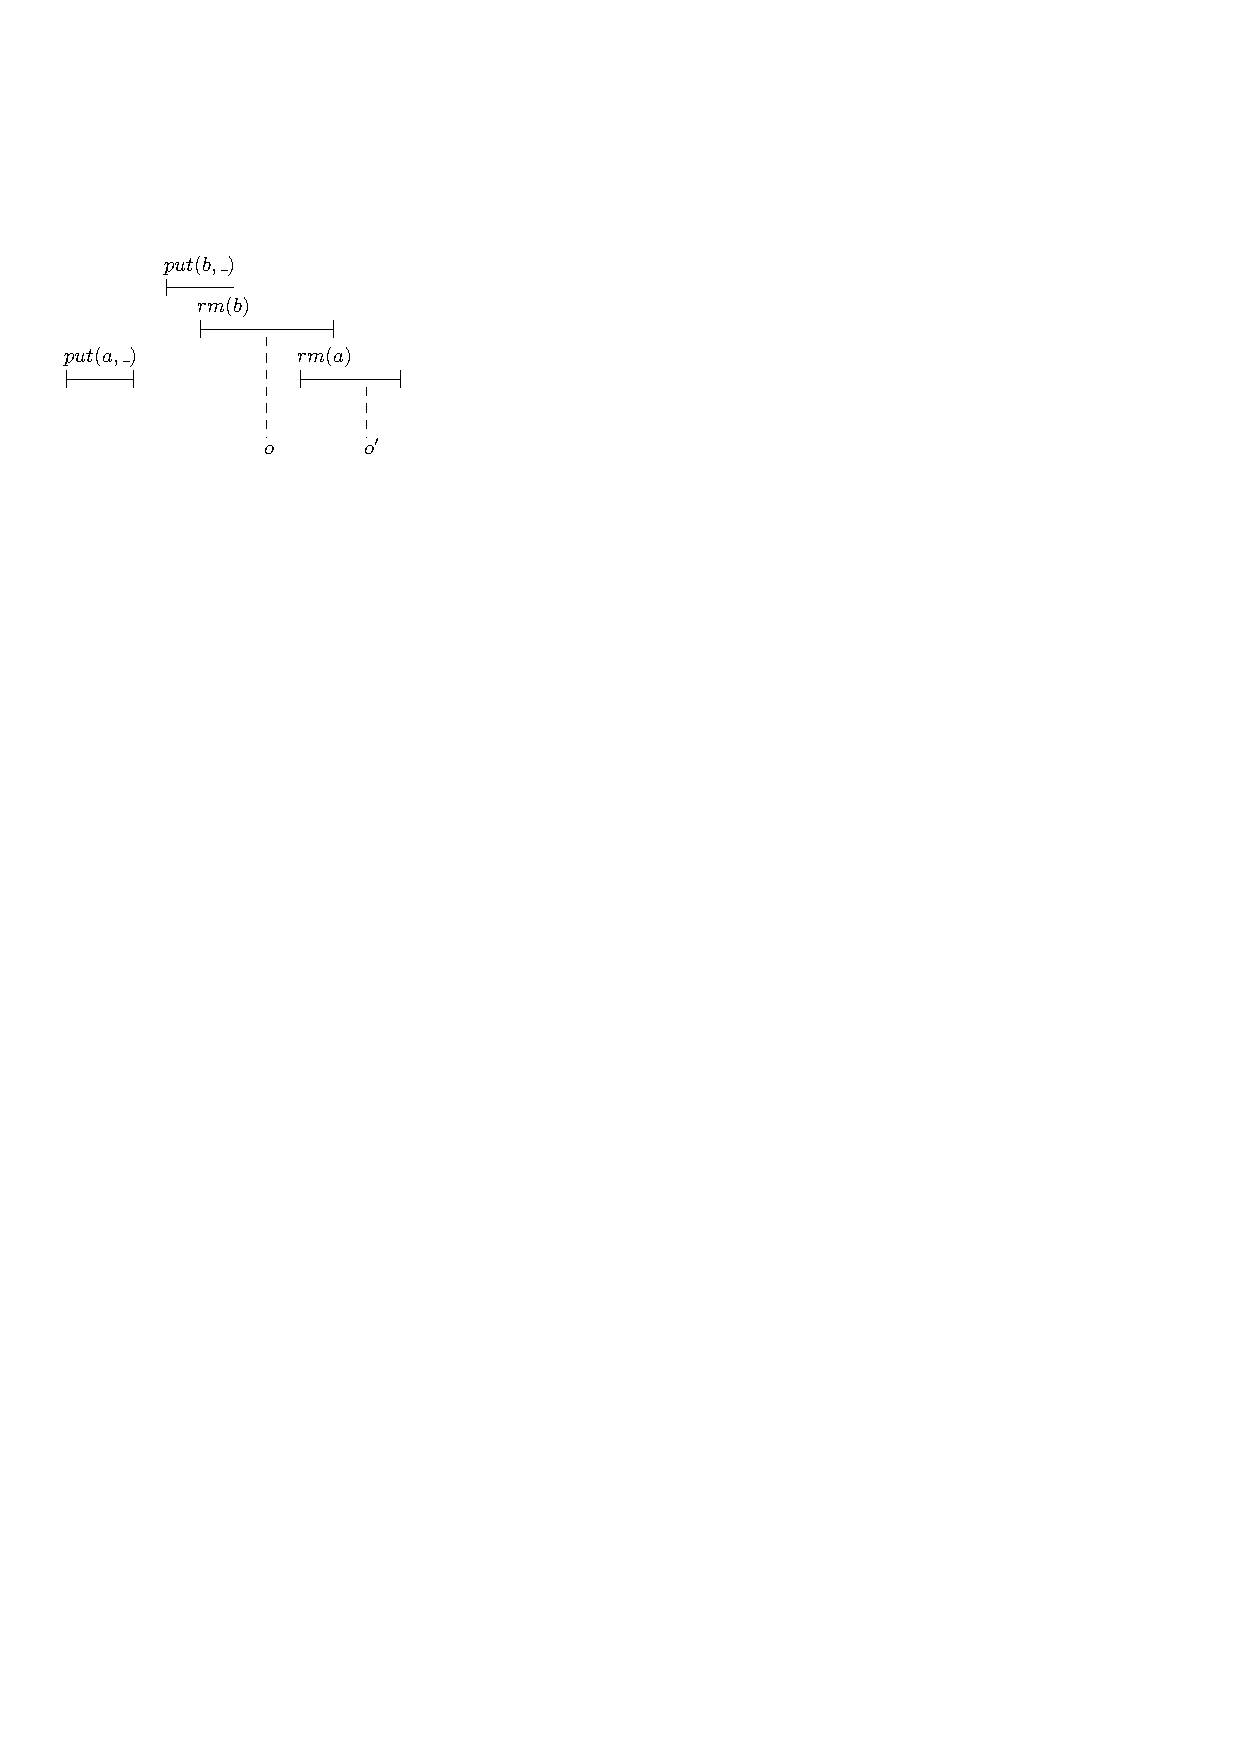
\includegraphics[width=0.4 \textwidth]{figures/PIC-HIS-PQ1Equal-1.pdf}
%\vspace{-10pt}
  \caption{The first possible enumeration.}
  \label{fig:history enumeration 1 for PQ1Equal}
\end{figure}


\begin{figure}[htbp]
  \centering
  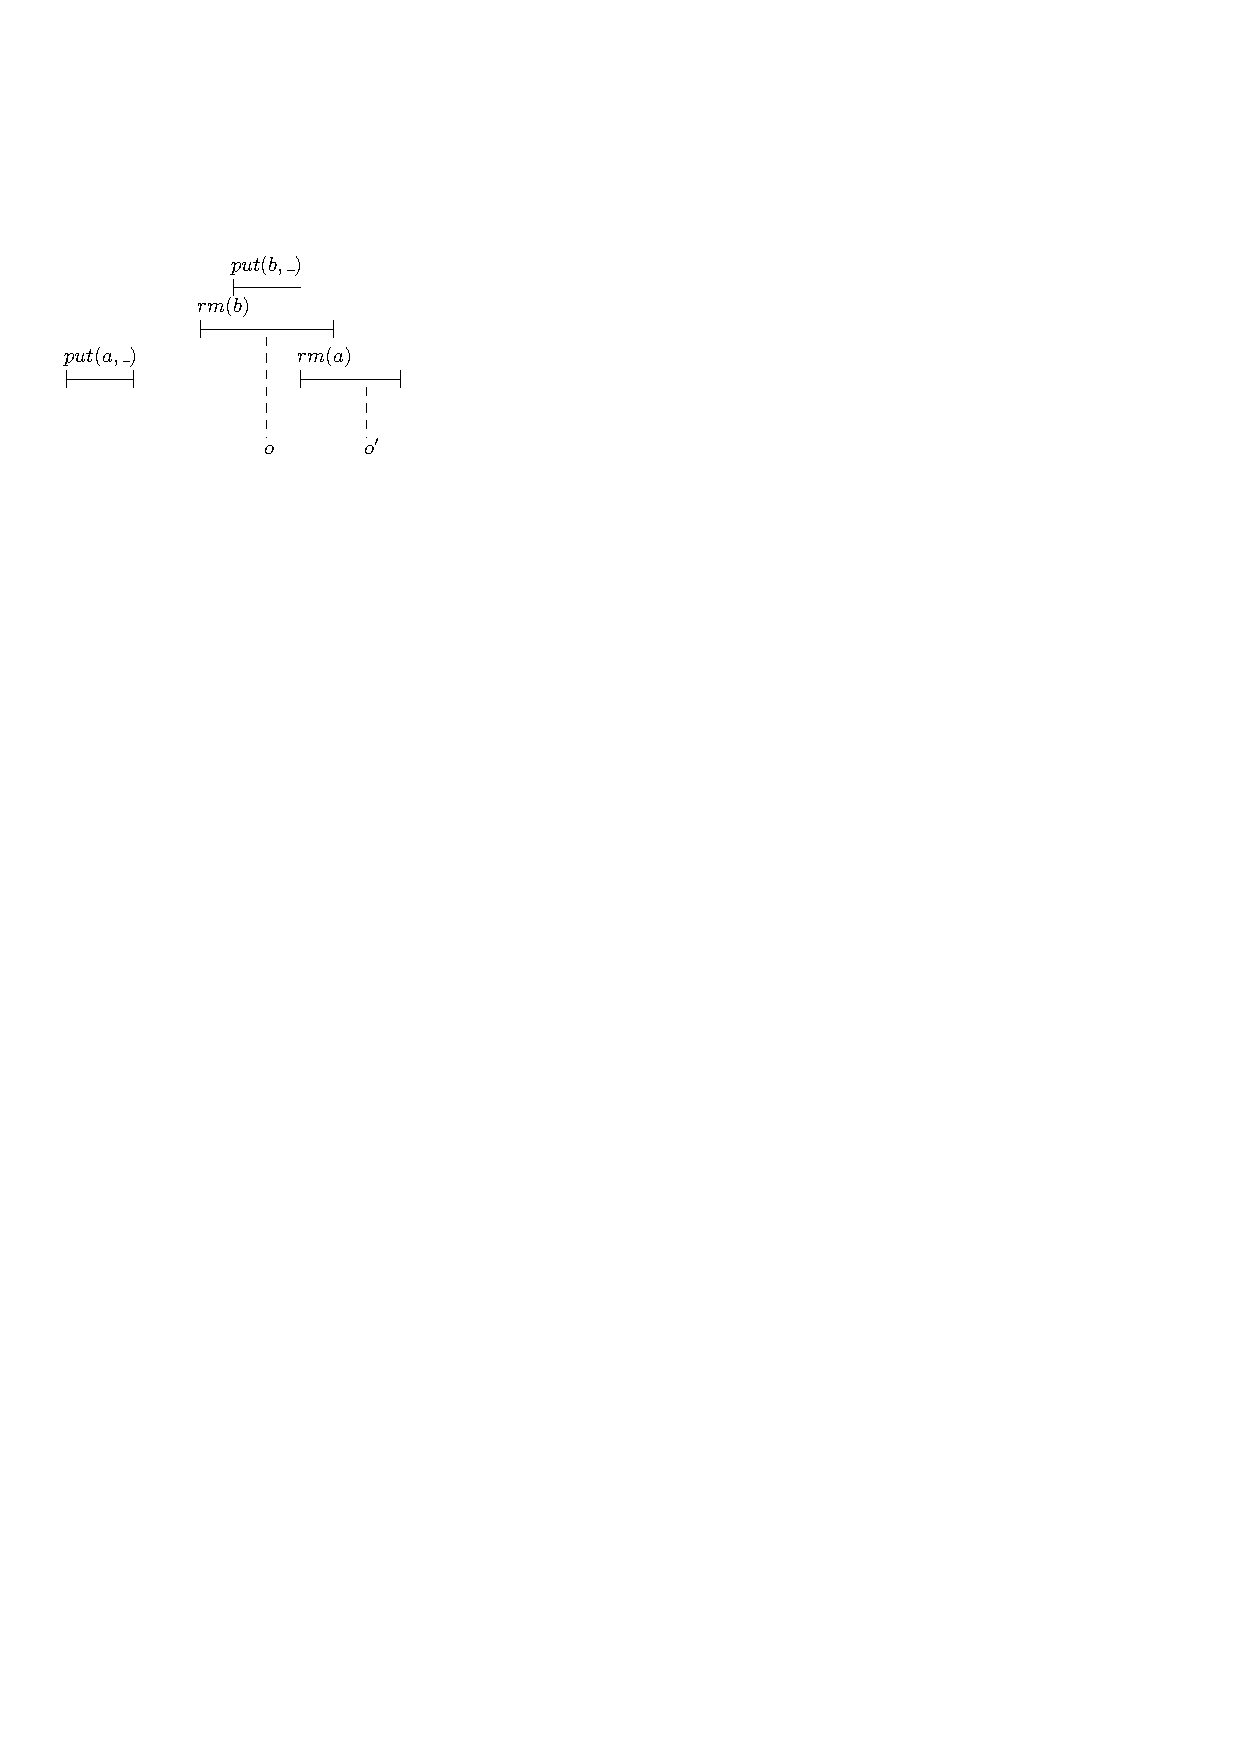
\includegraphics[width=0.4 \textwidth]{figures/PIC-HIS-PQ1Equal-2.pdf}
%\vspace{-10pt}
  \caption{The second possible enumeration.}
  \label{fig:history enumeration 2 for PQ1Equal}
\end{figure}

\begin{figure}[htbp]
  \centering
  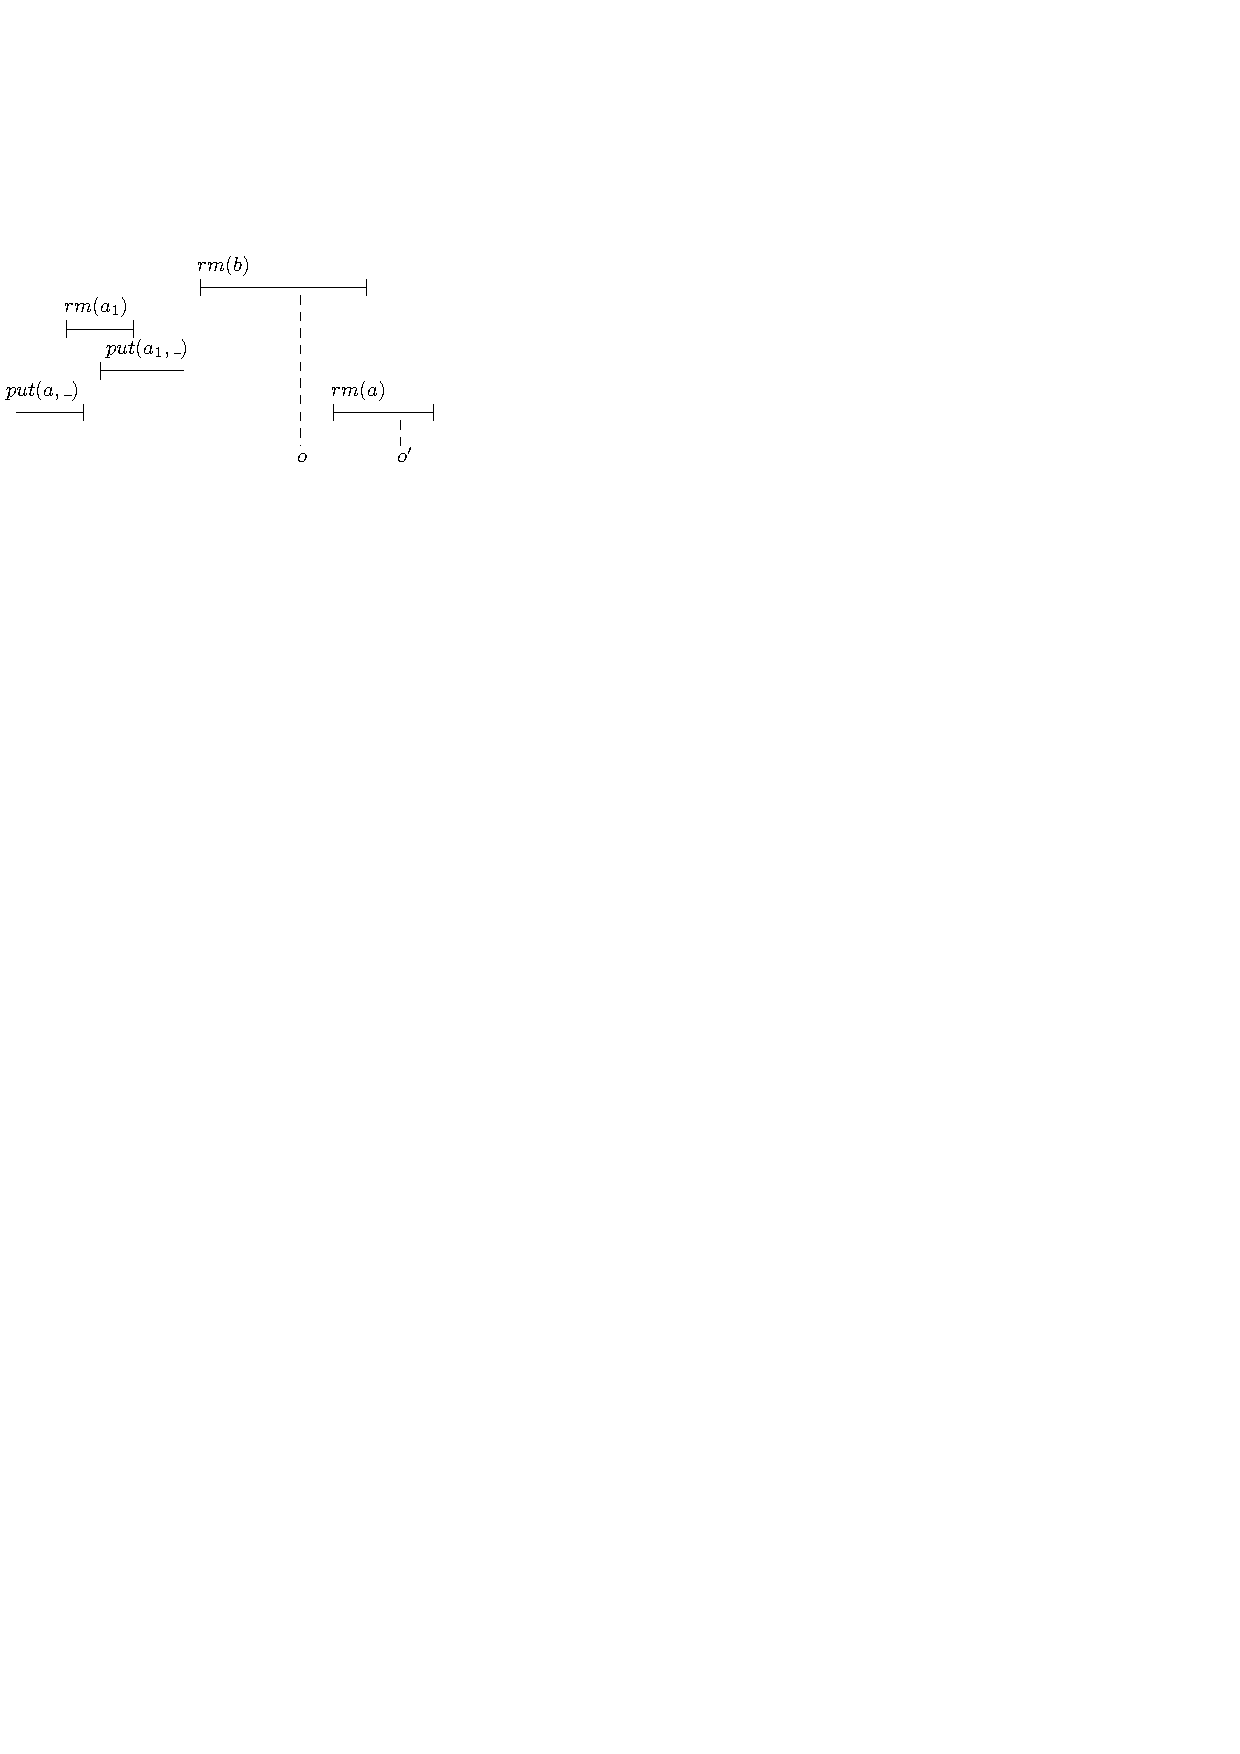
\includegraphics[width=0.4 \textwidth]{figures/PIC-HIS-PQ1Equal-3.pdf}
%\vspace{-10pt}
  \caption{The third possible enumeration.}
  \label{fig:history enumeration 3 for PQ1Equal}
\end{figure}

\begin{figure}[htbp]
  \centering
  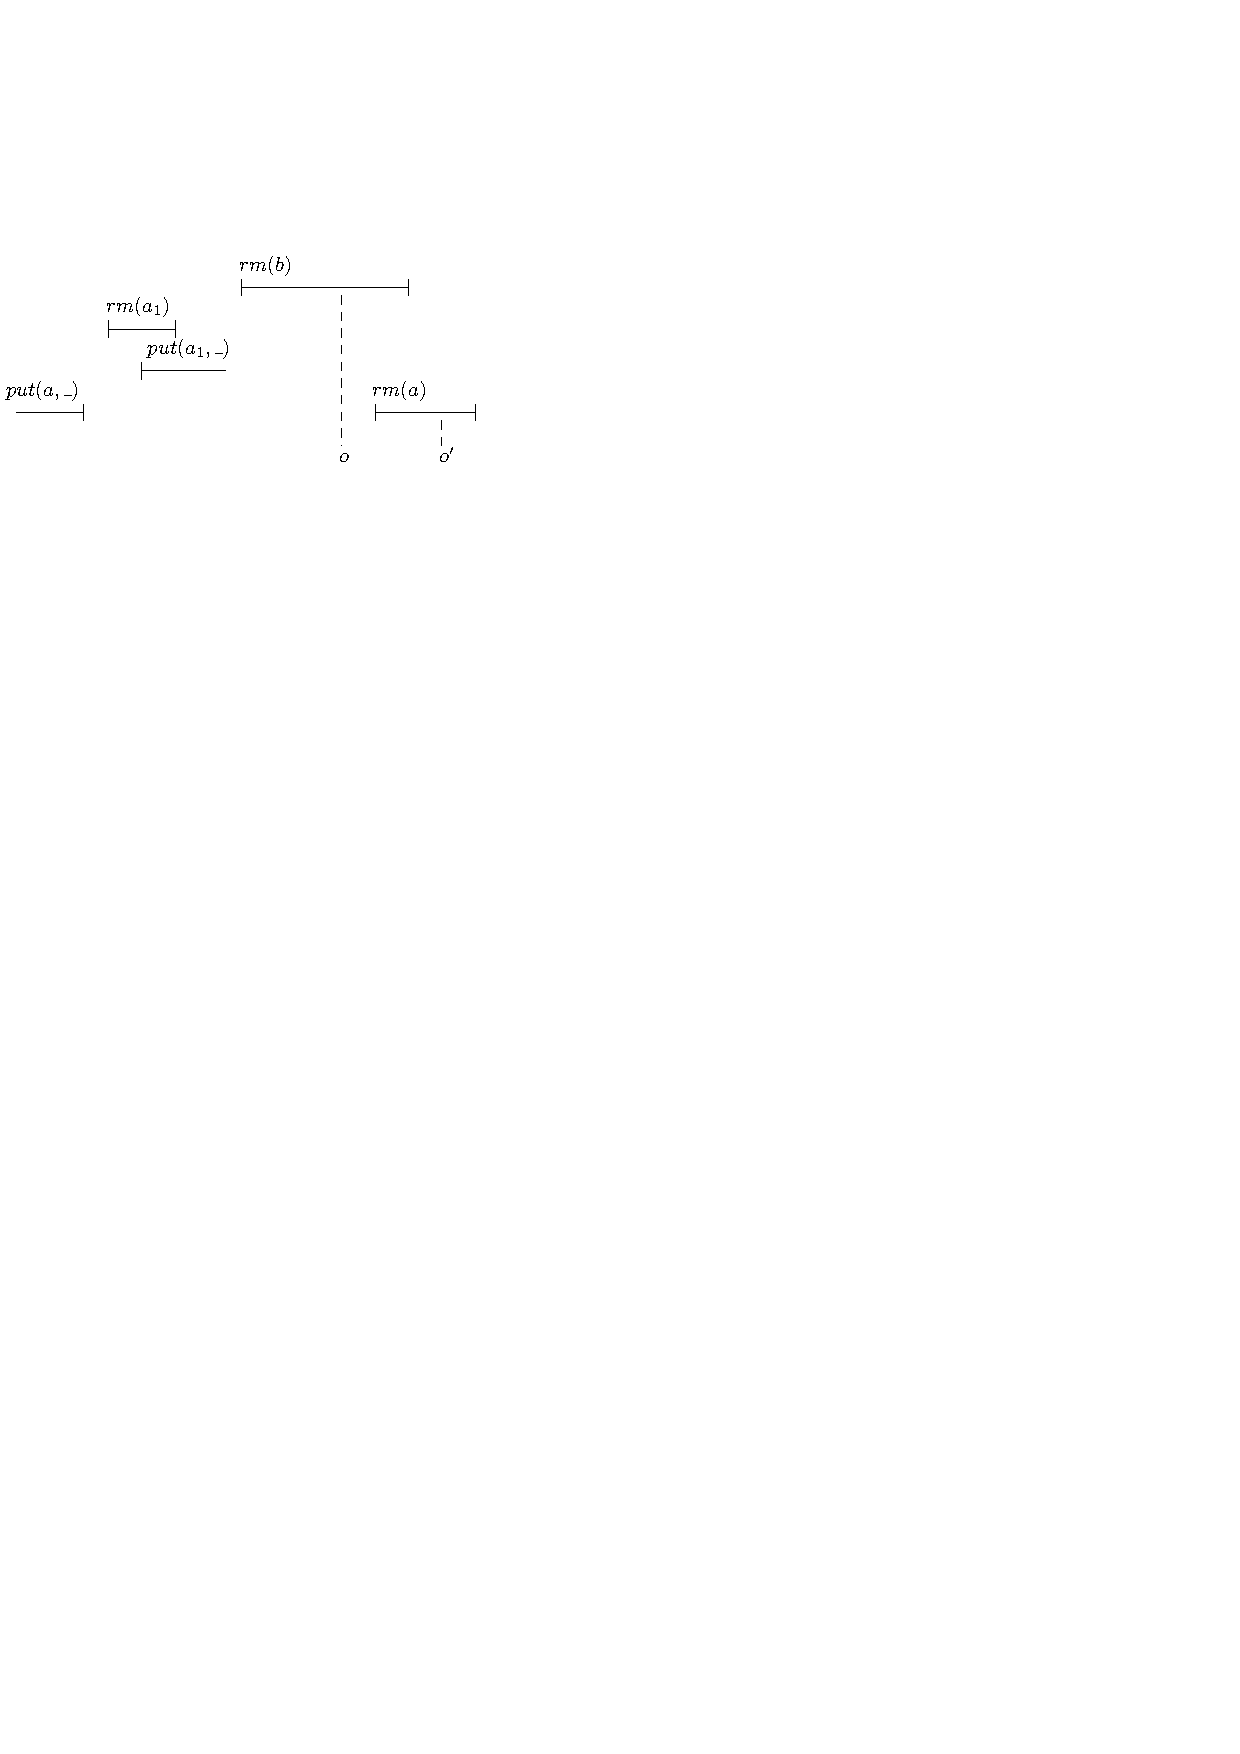
\includegraphics[width=0.4 \textwidth]{figures/PIC-HIS-PQ1Equal-4.pdf}
%\vspace{-10pt}
  \caption{The forth possible enumeration.}
  \label{fig:history enumeration 4 for PQ1Equal}
\end{figure}

\begin{figure}[htbp]
  \centering
  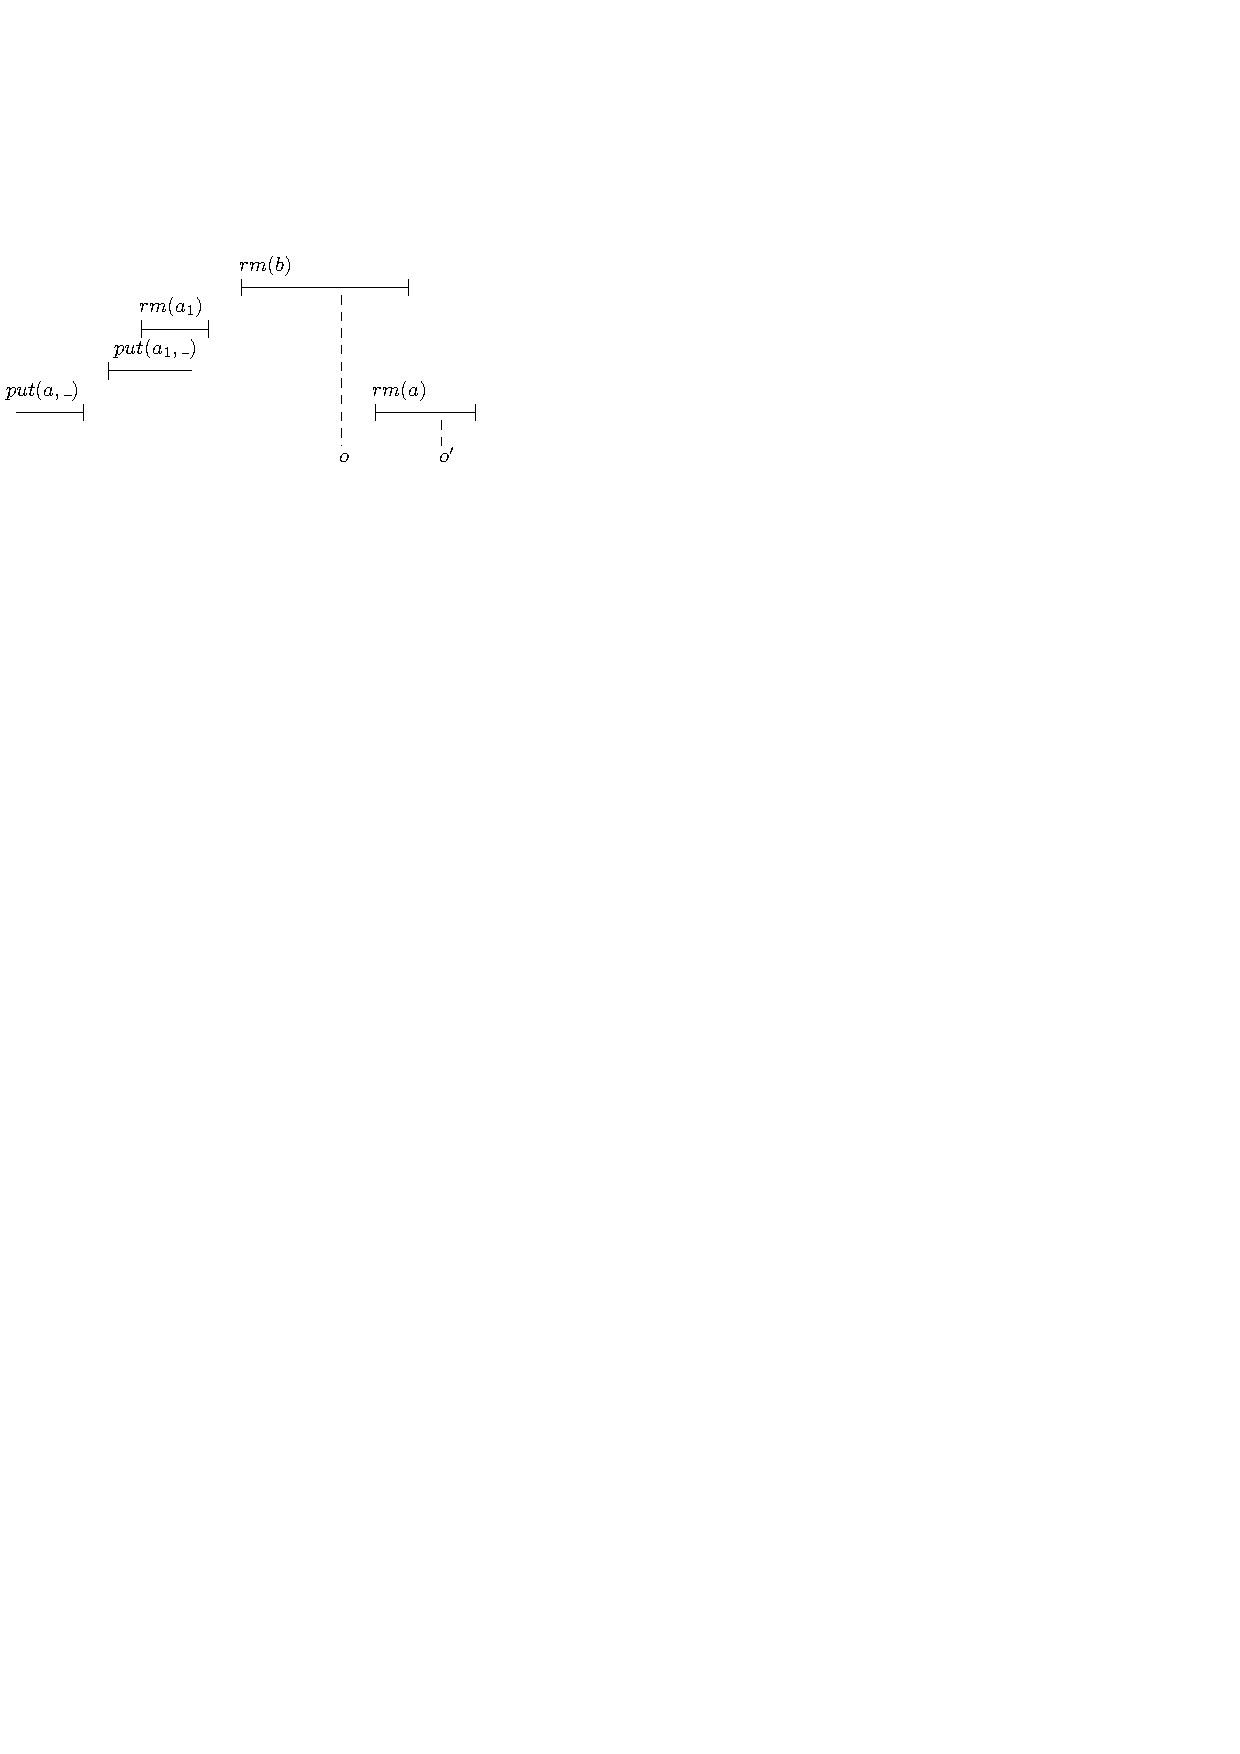
\includegraphics[width=0.4 \textwidth]{figures/PIC-HIS-PQ1Equal-5.pdf}
%\vspace{-10pt}
  \caption{The fifth possible enumeration.}
  \label{fig:history enumeration 5 for PQ1Equal}
\end{figure}


Let us begin to represent several register automata that is used to capture the existence of a data-differentiated $\_$-execution $e$, $e$ has a projection $e'$, $\textit{last}(e') = \seqPQ_1^{=}$, there exists items $a$ and $b$ with maximal priority in $e'$, $a <_{\textit{pb}}^* b$, and the rightmost gap-point of $b$ is before $\textit{call}(\textit{put},a,\_)$ or $\textit{call}(\textit{rm},a)$.

Given a data-differentiated $\_$-execution $e$, two actions $\textit{act}_1$, $\textit{act}_2$ of maximal priority in $e$, and assume that $\textit{act}_1$ is before $\textit{act}_2$ in $e$.
we say that $\textit{act}_1$, $\textit{act}_2$ is covered by items $d_1,\ldots,d_m$ in $e$, if the priorities of $d_1,\ldots,d_m$ is smaller than that of $\textit{act}_1$ and $\textit{act}_2$, and

\begin{itemize}
\setlength{\itemsep}{0.5pt}
\item[-] $\textit{ret}(\textit{put},d_m,\_)$ is before $\textit{act}_1$,

\item[-] For each $i < 1 \leq m$,$\textit{put}(d_{\textit{i-1}},\_)$ happens before $\textit{rm}(d_i)$,

\item[-] $\textit{act}_2$ is before $\textit{call}(\textit{rm},d_1)$.
\end{itemize}

According to Lemma \ref{lemma:EPQ1Equal as pb order and gap-point}, Lemma \ref{lemma:ob order has bounded length} and Lemma \ref{lemma:five enumeration is enough for EPQ1Equal}, it is not hard to prove that, given a data-differentiated $\_$-execution $e$ with $\textit{last}(e) = \seqPQ_1^{=}$, $e$ does not linearizable with respect to $\textit{EMS}(\textit{PQ}_1^{=})$, if and only if, one of enumerations holds in $e$ (permit renaming), while $\textit{call}(\textit{rm},a)$ and $\textit{ret}(\textit{rm},b)$ is covered by some $d_1,\ldots,d_m$, $\textit{call}(\textit{rm},b)$ is before $\textit{ret}(\textit{put},d_m,\_)$, and $\textit{call}(\textit{rm},d_1)$ is before $\textit{ret}(\textit{rm},a)$. We say that such $d_1,\ldots,d_m$ constitute the rightmost gap of $b$.


An automaton $\mathcal{A}_{\textit{l-eq}}^1$ is given in \figurename~\ref{fig:automata for first enumeration of PQ1Equal}, and it is constructed for the first enumeration in \figurename~\ref{fig:history enumeration 1 for PQ1Equal}. Here we rename the items that covers $\textit{call}(\textit{rm},a)$ and $\textit{ret}(\textit{rm},b)$ into $d$, and rename the remanning items into $e$. In this figure, $c = \textit{call}(\textit{put},e,\textit{anyPri}),\textit{ret}(\textit{put},e)$, $\textit{call}(\textit{rm},e), \textit{ret}(\textit{rm},e),\textit{call}(\textit{rm},\textit{empty}),\textit{ret}(\textit{rm},\textit{empty})$, $c_1 = c + \textit{call}(\textit{put},d,\textit{les}_p)$, $c_2 = c_1 + \textit{ret}(\textit{put},b)$, $c_3 = c_2 + \textit{call}(\textit{put},d),\textit{ret}(\textit{rm},d)$, $c_4 = c + \textit{ret}(\textit{put},b) + \textit{ret}(\textit{rm},d)$.

\begin{figure}[htbp]
  \centering
  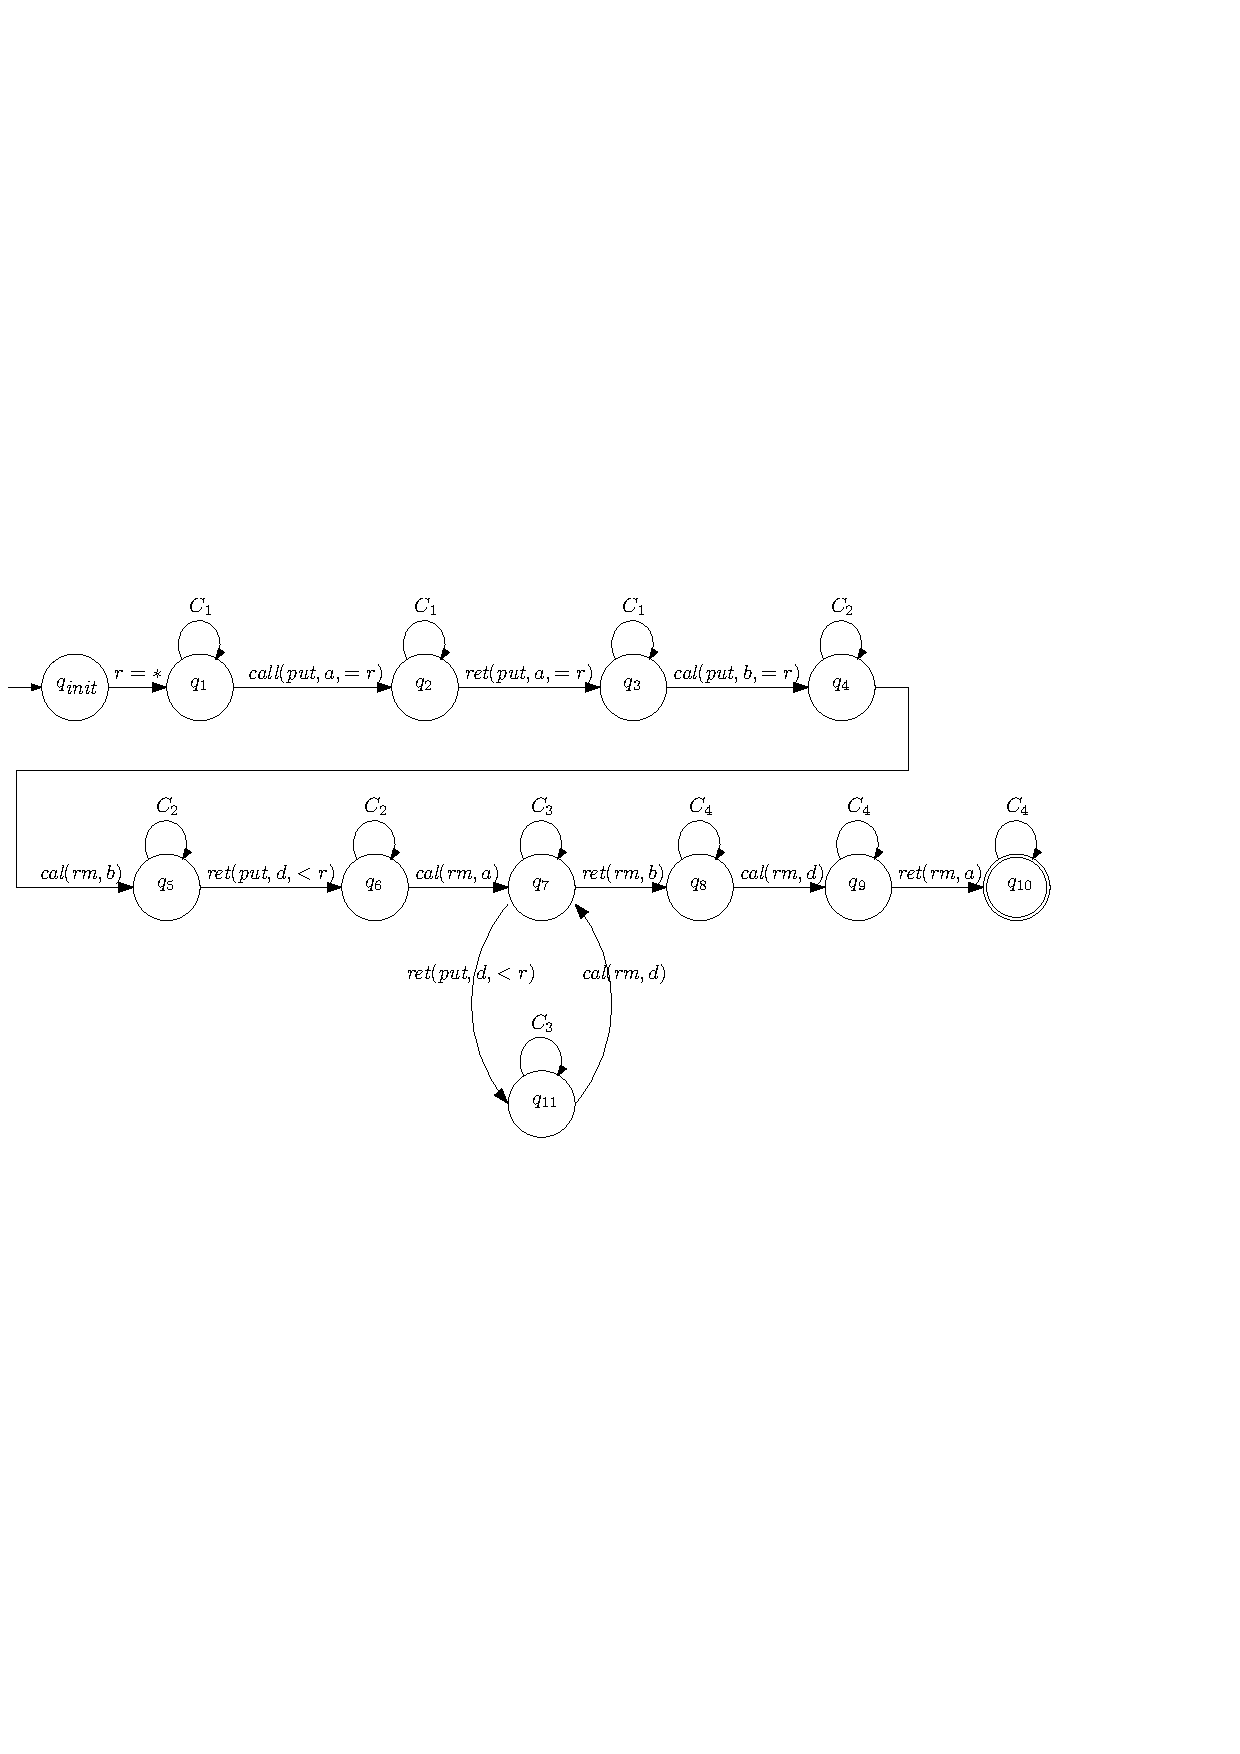
\includegraphics[width=0.8 \textwidth]{figures/PIC_AUTO_PQ1Equ-1.pdf}
%\vspace{-10pt}
  \caption{Automaton $\mathcal{A}_{\textit{l-eq}}^1$}
  \label{fig:automata for first enumeration of PQ1Equal}
\end{figure}


An automaton $\mathcal{A}_{\textit{l-eq}}^2$ is given in \figurename~\ref{fig:automata for second enumeration of PQ1Equal}, and it is constructed for the second enumeration in \figurename~\ref{fig:history enumeration 2 for PQ1Equal}. In \figurename~\ref{fig:automata for second enumeration of PQ1Equal}, $c_1$, $c_2$, $c_3$ and $c_4$ is same as that in \figurename~\ref{fig:automata for first enumeration of PQ1Equal}.

\begin{figure}[htbp]
  \centering
  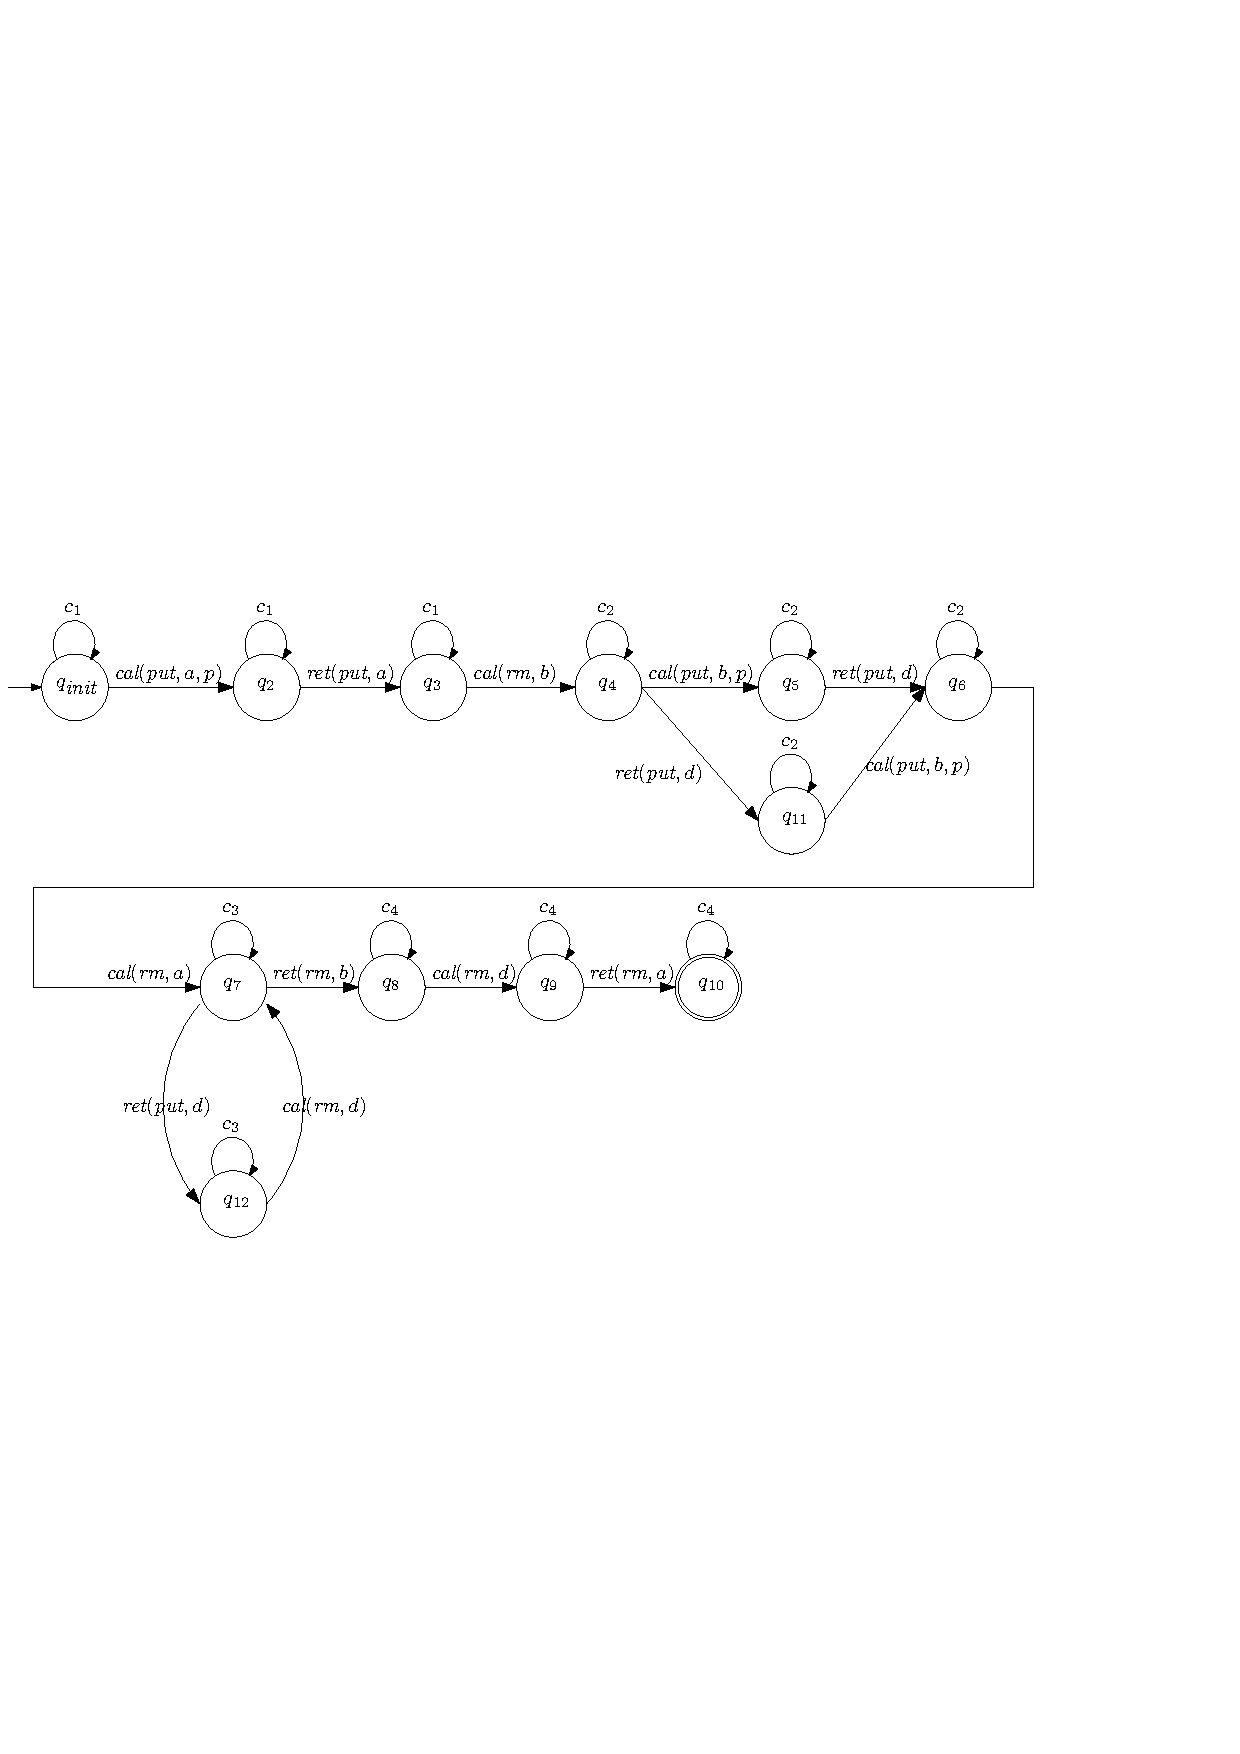
\includegraphics[width=0.8 \textwidth]{figures/PIC_AUTO_PQ1Equ-2.pdf}
%\vspace{-10pt}
  \caption{Automaton $\mathcal{A}_{\textit{l-eq}}^2$}
  \label{fig:automata for second enumeration of PQ1Equal}
\end{figure}

For the third enumeration in \figurename~\ref{fig:history enumeration 3 for PQ1Equal}. Since we want to ensure that $a$ and $b$ are putted only once, we need to explicitly record the positions of $\textit{call}(\textit{put},a,p)$ and $\textit{call}(\textit{put},b,p)$. Since the positions of $\textit{call}(\textit{put},a,p)$ and $\textit{call}(\textit{put},b,p)$ are not fixed, there are finite possible cases to consider, as shown below:

\begin{itemize}
\setlength{\itemsep}{0.5pt}
\item[-] If $\textit{call}(\textit{put},b,p)$ is after $\textit{call}(\textit{rm},b)$ and before $\textit{call}(\textit{rm},a)$: There are two possible positions of $\textit{call}(\textit{put},a,p)$: (1) before $\textit{call}(\textit{rm},a_1)$, and (2) after $\textit{call}(\textit{rm},a_1)$, and before $\textit{ret}(\textit{put},a)$.

\item[-] If $\textit{call}(\textit{put},b,p)$ is after $\textit{ret}(\textit{rm},a_1)$ and before $\textit{call}(\textit{rm},b)$: same as above case.

\item[-] If $\textit{call}(\textit{put},b,p)$ is after $\textit{call}(\textit{put},a_1,\_)$ and before $\textit{ret}(\textit{rm},a_1)$: same as above case.

\item[-] If $\textit{call}(\textit{put},b,p)$ is after $\textit{ret}(\textit{put},a)$ and before $\textit{call}(\textit{put},a_1,p)$: same as above case.

\item[-] If $\textit{call}(\textit{put},b,p)$ is after $\textit{call}(\textit{rm},a_1)$ and before $\textit{ret}(\textit{put},a)$: There are three possible positions of $\textit{call}(\textit{put},a,p)$: (1) after $\textit{call}(\textit{put},b,p)$ and before $\textit{ret}(\textit{put},a)$, (2) after $\textit{call}(\textit{rm},a_1)$ and before $\textit{call}(\textit{put},b,p)$, and (3) before $\textit{call}(\textit{rm},a_1)$.

\item[-] If $\textit{call}(\textit{put},b,p)$ is before $\textit{call}(\textit{rm},a_1)$: There are three possible positions of $\textit{call}(\textit{put},a,p)$: (1) after $\textit{call}(\textit{rm},a_1)$ and before $\textit{ret}(\textit{put},a)$, (2) after $\textit{call}(\textit{put},b,p)$ and before $\textit{call}(\textit{rm},a_1)$, and (3) before $\textit{call}(\textit{put},b,p)$.
\end{itemize}

Therefore, there are fourteen possible cases that satisfy the third enumeration in \figurename~\ref{fig:history enumeration 3 for PQ1Equal}. For each case, we construct an finite automaton. Let $\textit{Auts}_{\textit{1-eq}}^{3}$ be the set of finite automata that is constructed for above fourteen cases. For example, for the case $\textit{ca}_1$ when $\textit{call}(\textit{put},a,p)$ is before $\textit{call}(\textit{rm},a_1)$, $\textit{call}(\textit{put},b,p)$ is after $\textit{ret}(\textit{rm},a_1)$, and $\textit{call}(\textit{put},b,p)$ is before $\textit{call}(\textit{rm},b)$, we construct a finite automaton $\mathcal{A}_{\textit{l-eq}}^{\textit{3-1}}$ in \figurename~\ref{fig:automata for ca1 of third enumeration of Rpr2}. In \figurename~\ref{fig:automata for ca1 of third enumeration of Rpr2}, let $c$ and $c_1 = c + \textit{call}(\textit{put},d,\textit{les}_p)$ the same as that in \figurename~\ref{fig:automata for first enumeration of PQ1Equal}. Let $c_2 = c_1 + \textit{ret}(\textit{put},a_1)$, $c_3 = c_2 + \textit{ret}(\textit{put},b)$, $c_4 = c_3 + \textit{call}(\textit{put},d) + \textit{ret}(\textit{rm},d)$, and $c_5 = c + \textit{ret}(\textit{put},b) + \textit{ret}(\textit{put},a_1) + \textit{ret}(\textit{rm},d)$. The other register automata in $\textit{Auts}_{\textit{1-eq}}^{3}$ can be similarly constructed.

\begin{figure}[htbp]
  \centering
  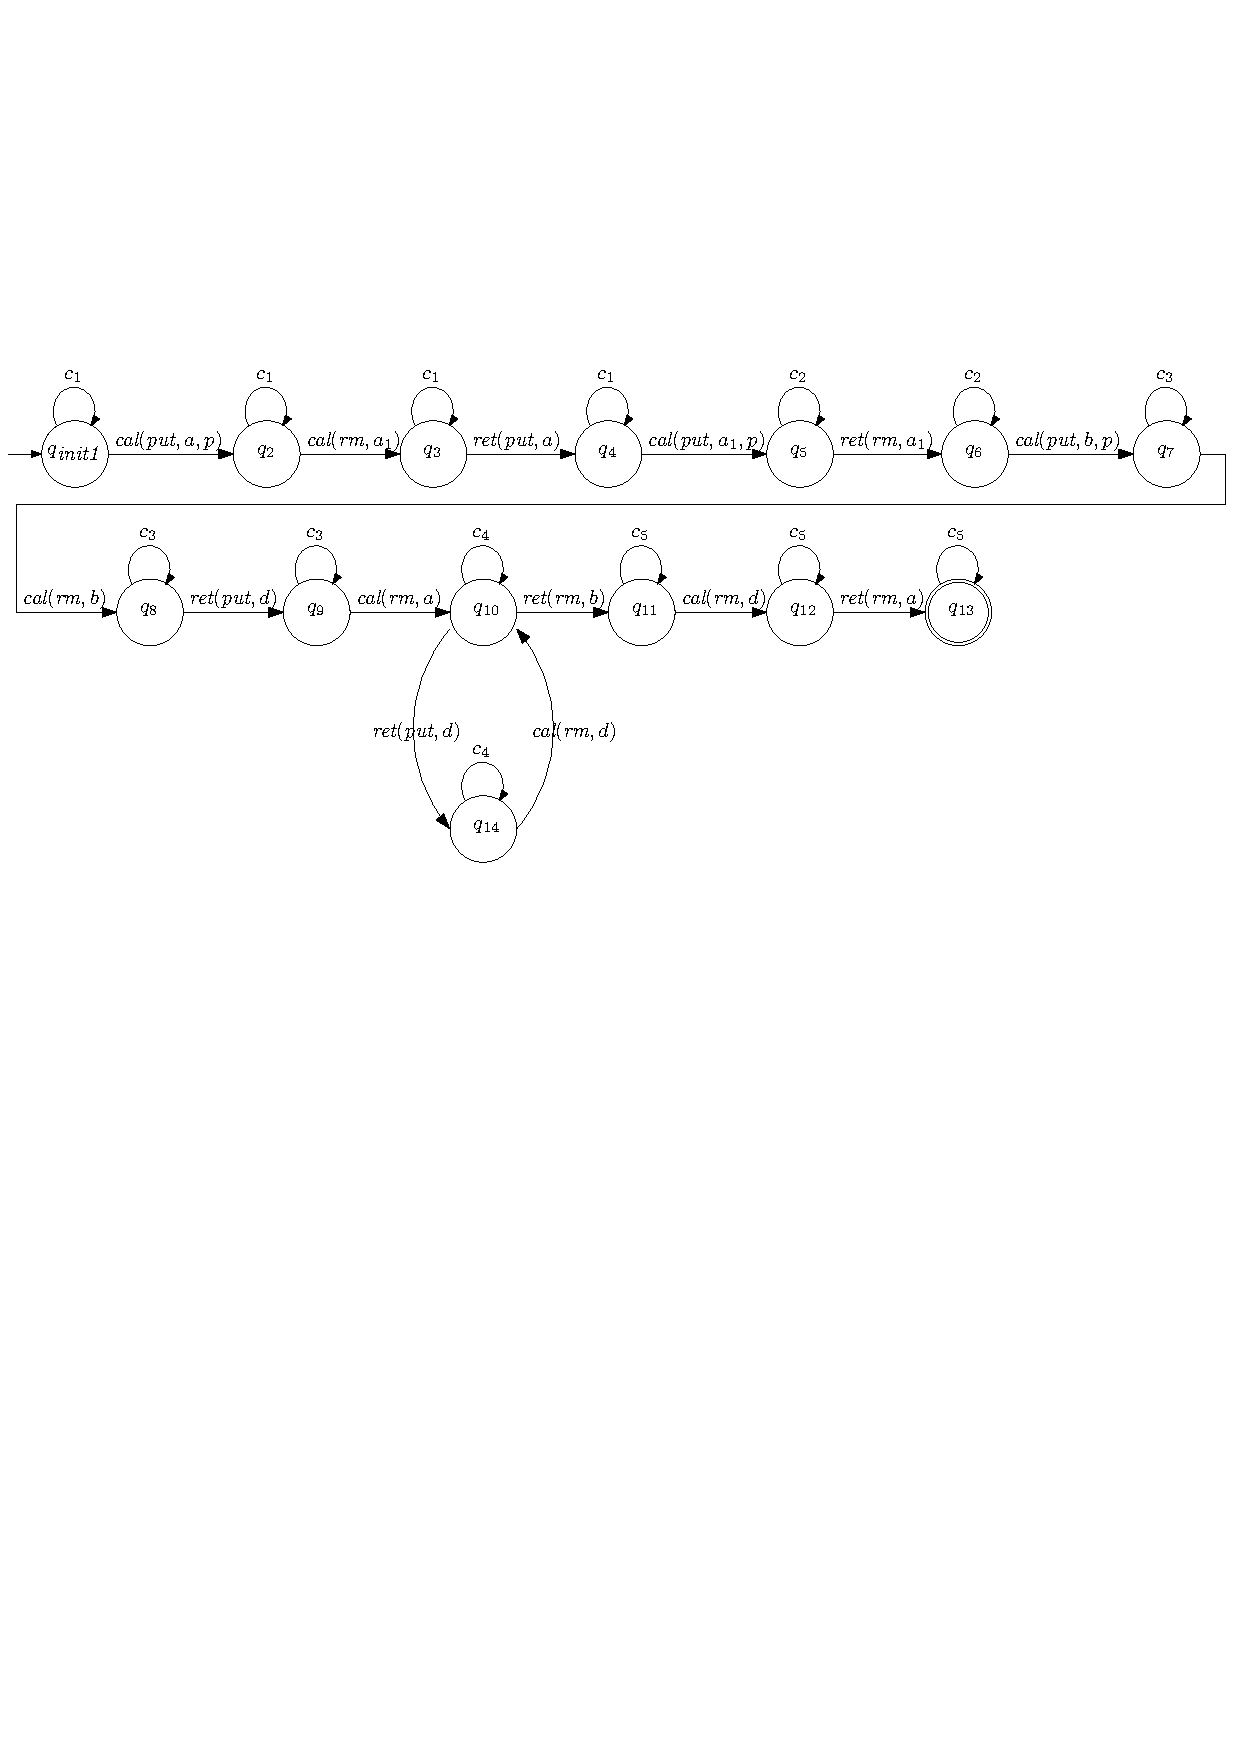
\includegraphics[width=0.8 \textwidth]{figures/PIC_AUTO_PQ1Equ-3-1.pdf}
%\vspace{-10pt}
  \caption{Automaton $\mathcal{A}_{\textit{l-eq}}^{\textit{3-1}}$}
  \label{fig:automata for ca1 of third enumeration of Rpr2}
\end{figure}

Similarly, we construct sets $\textit{Auts}_{\textit{1-eq}}^{4}$ and $\textit{Auts}_{\textit{1-eq}}^{5}$ of register automata for the forth enumeration in \figurename~\ref{fig:history enumeration 4 for PQ1Equal} and the fifth enumeration in \figurename~\ref{fig:history enumeration 5 for PQ1Equal}, respectively.

Let $\textit{Auts}_{\textit{1-eq}} = \{ \mathcal{A}_{\textit{l-eq}}^1, \mathcal{A}_{\textit{l-eq}}^2 \} \cup \textit{Auts}_{\textit{1-eq}}^{3} \cup \textit{Auts}_{\textit{1-eq}}^{4} \cup \textit{Auts}_{\textit{1-eq}}^{5}$. The following lemma states that $\textit{PQ}_1^{=}$ is co-regular.


\begin{restatable}{lemma}{EPQOneEqualIsCoRegular}
\label{lemma:EPQ1Equal is co-regular}
$\mathsf{MatchedMaxPriority}^{=}$ is co-regular.
\end{restatable}

\begin {proof}

We need to prove that, given a data-independence implementation $\mathcal{I}$, $\textit{Auts}_{\textit{1-eq}} \cap \mathcal{I} \neq \emptyset$, if and only if $\exists e \in \mathcal{I}_{\neq},$ $e' \in \textit{proj}(e),$ $\seqPQ_1^{=} \in \textit{last}(e') \wedge e'$ does not linearizable w.r.t. $\textit{MS}(\seqPQ_1^{=})$.

By Lemma \ref{lemma:pri execution is enough} and Lemma \ref{lemma:EPQ1Equal as pb order and gap-point}, we need to prove the following fact:

\noindent {\bf $\textit{fact}_1$}: Given a data-independence implementation $\mathcal{I}$, $\textit{Auts}_{\textit{1-eq}} \cap \mathcal{I} \neq \emptyset$ if and only if $\exists e \in \mathcal{I}_{\neq},$ $e' \in \textit{proj}(e)$, $\textit{last}(e')=\seqPQ_1^{=}$, $a$ and $b$ are two items with maximal priority $p$ in $e'$, $e'$ is a $p$-execution, $a <_{\textit{pb}}^* b$ in $e'$, and the rightmost gap-point of $b$ is before $\textit{call}(\textit{put},a,p)$ or $\textit{call}(\textit{rm},a)$ in $e'$.

\noindent The $\textit{only if}$ direction: Assume that $e_1 \in \mathcal{I}$ is accepted by some register automata in $\textit{Auts}_{\textit{1-eq}}$. By data-independence, there exists data-differentiated execution $e_2 \in \mathcal{I}$ and a renaming function $r$, such that $e_1=r(e_2)$. Since $e_1$ is accepted by some register automata in  $\textit{Auts}_{\textit{1-eq}}$, let $x$, $y$ and $z$ (if exists) be the items that are renamed into $b$, $a$ and $a_1$ (if exists) by $r$, respectively, and let $d_1,\ldots,d_m$ be the items that are renamed into $d$ by $r$.

let $e'' = e_2 \vert_{ \{ x,y,z,d_1,\ldots,d_m \} }$. It is obvious that $e'' \in \textit{proj}(e_2)$ is a $p$-execution, $\textit{last}(e'') = \seqPQ_1^{=}$. According to our construction of automata in $\textit{Auts}_{\textit{1-eq}}$, it is not hard to see that $x$ and $y$ has maximal priority in $h_2$, $y <_{\textit{pb}}^* x$, and the rightmost gap-point of $x$ is before $\textit{call}(\textit{put},y,p)$ or $\textit{call}(\textit{rm},y)$ in $e''$.

\noindent The $\textit{if}$ direction: Assume that there exists $e \in \mathcal{I}_{\neq},e' \in \textit{proj}(e)$, such that $last(e')=\textit{PQ}_1^{=}$, $a'$ and $b'$ are two items with maximal priority $p$ in $e'$, $e'$ is a $p$-execution, $a' <_{\textit{pb}}^* b'$ in $e'$, and the rightmost gap-point of $b'$ is before $\textit{call}(\textit{put},a',p)$ or $\textit{call}(\textit{rm},a')$ in $e'$. By data-independence, we can obtain execution $e_1$ as follows: (1) rename $a'$ and $b'$ into $a$ and $b$, respectively, (2) for the items $d_1,\ldots,d_m$ that constitute the rightmost gap of $b'$, we rename them into $d$, (3) if $a' <_{\textit{pb}}^A a'_1 <_{\textit{pb}}^B b$, we rename $a'_1$ into $a_1$, and (4) rename the other items into $e$. It is easy to see that $\textit{last}(e_1) = \seqPQ_1^{=}$, $a$ and $b$ has maximal priority in $e_1$, $a <_{\textit{pb}}^* b$ in $e_1$, and the rightmost gap-point of $b$ is before $\textit{call}(\textit{put},a,p)$ or $\textit{call}(\textit{rm},a)$ in $e_1$. By Lemma \ref{lemma:five enumeration is enough for EPQ1Equal}, there are five possible enumeration of operations of $a$, $b$, $a_1$ (if exists). Then


\begin{itemize}
\setlength{\itemsep}{0.5pt}
\item[-] If $a <_{\textit{pb}}^* b$ because of the first enumeration, it is easy to see that $h_1$ is accepted by $\mathcal{A}_{\textit{l-eq}}^1$.

\item[-] If $a <_{\textit{pb}}^* b$ because of the second enumeration, it is easy to see that $h_1$ is accepted by $\mathcal{A}_{\textit{l-eq}}^2$.

\item[-] If $a <_{\textit{pb}}^* b$ because of the third enumeration, it is easy to see that $h_1$ is accepted by some register automaton in $\textit{Auts}_{\textit{1-eq}}^{3}$.

\item[-] If $a <_{\textit{pb}}^* b$ because of the forth enumeration, it is easy to see that $h_1$ is accepted by some register automaton in $\textit{Auts}_{\textit{1-eq}}^{4}$.

\item[-] If $a <_{\textit{pb}}^* b$ because of the fifth enumeration, it is easy to see that $h_1$ is accepted by some register automaton in $\textit{Auts}_{\textit{1-eq}}^{5}$.
\end{itemize}

This completes the proof of this lemma. \qed
\end {proof}





\subsection{Co-Regular of $\seqPQ_2^{>}$}
\label{subsec:appendix co-regular of EPQ2Lar}


\begin{restatable}{lemma}{EPQ2LarIsAlwaysCoRegular}
\label{lemma:EPQ2Lar is always co-regular}
Given a data-differentiated $\_$-execution $e$, if $\textit{last}(e) = \seqPQ_2^{>}$, then $e \sqsubseteq \textit{MS}(\seqPQ_2^{>})$.
\end{restatable}

\begin {proof}
Since $\textit{last}(e) = \seqPQ_2^{>}$, the actions with maximal priority in $e$ is some unmatched $\textit{put}$. Therefore, no matter how we locate linearization points, we can always obtain a sequence $l$ of operations that contains unmatched $\textit{put}$ with maximal priority, and this satisfy the guard of $\textit{MS}(\seqPQ_2^{>})$. This completes the proof of this lemma. \qed
\end {proof}




\subsection{Co-Regular of $\seqPQ_2^{=}$}
\label{subsec:appendix co-regular of EPQ2Equal}

\begin{restatable}{lemma}{EPQ2EqualAsHappenBefore}
\label{lemma:EPQ2Equal as happen before}
Given a data-differentiated $p$-execution $e$ with $\textit{last}(e) = \seqPQ_2^{=}$. $e$ does not linearizable to $\textit{MS}(\seqPQ_2^{=})$, if and only if there exists $x$ and $y$ with priority $p$, $x$ has unmatched $\textit{put}$, $y$ has matched $\textit{put}$ and $\textit{rm}$, and $\textit{put}(x,p) <_{\textit{hb}} \textit{put}(y,p)$.
\end{restatable}

\begin {proof}

The $\textit{if}$ direction is obvious.

To prove the $\textit{only if}$ direction, we prove its contrapositive. Assume that for each pair of $x$ and $y$ with maximal priority in $e$, if $x$ has unmatched $\textit{put}$, $y$ has matched $\textit{put}$ and $\textit{rm}$, then $\textit{put}(x,p)$ does not happen before $\textit{put}(y,p)$. We need to prove that $e \sqsubseteq \textit{MS}(\seqPQ_2^{=})$.

Let $x_1,\ldots,x_m$ be the set of items with priority $p$ and has unmatched $\textit{put}$ in $e$, let $y_1,\ldots,y_n$ be the set of items with priority $p$ and has matched $\textit{put}$ and $\textit{rm}$ in $e$. By assumption, we know that $\textit{call}(\textit{put},y_i,p)$ is before $\textit{ret}(\textit{put},x_j)$ for each $i,j$. Then we explicitly construction the linearization of $e$ by locating the linearization points of $e$ as follows:

\begin{itemize}
\setlength{\itemsep}{0.5pt}
\item[-] For each $x_i$, locate the linearization point of $\textit{put}(x_i,p)$ just before its return action.

\item[-] For each $y_j$, locate the lineariztion point of $\textit{put}(y_j,p)$ jest after its call action.

\item[-] For other operations, locate their linearization points at an arbitrary location after its call action and before its return action.
\end{itemize}

Let $l$ be the sequence of linearization points. It is easy to see that $e \sqsubseteq l$. Since linearization points of $\textit{put}(x_i,p)$ is after the linearization point of $\textit{put}(y_j,p)$ for each $i,j$, it is easy to see that $l \in \textit{MS}(\seqPQ_2^{=})$. This completes the proof of this lemma. \qed
\end {proof}

Lemma \ref{lemma:EPQ2Equal as happen before} shows how to check violation to $\textit{MS}(\seqPQ_2^{=})$. However, the case in Lemma \ref{lemma:EPQ2Equal as happen before} violates our assumption that each single-priority execution is FIFO. Therefore, we know that $\seqPQ_2^{=}$ is always co-regular, as states by the following lemma.

\begin{restatable}{lemma}{EPQ2EqualIsAlwaysCoRegular}
\label{lemma:EPQ2Equal is always co-regular}
Given a data-differentiated $p$-execution $e$, if $\textit{last}(e) = \seqPQ_2^{=}$, then $e \sqsubseteq \textit{MS}(\seqPQ_2^{=})$.
\end{restatable}

\begin {proof}

According to Lemma \ref{lemma:EPQ2Equal as happen before}, if $\textit{last}(e) = \seqPQ_2^{=}$ and $e$ does not linearizable to $\textit{MS}(\seqPQ_2^{=})$, then there exists $x$ and $y$ with priority $p$, $x$ has unmatched $\textit{put}$, $y$ has matched $\textit{put}$, and $\textit{put}(x,p) <_{\textit{hb}} \textit{put}(y,p)$. Let $e_1 = e \vert_{ \{ x,y \} }$. It is obvious that $e_1$ does not satisfy FIFO property. This contradicts the assumption that every single-priority execution has FIFO property, and thus, we can safely ignore this case. \qed
\end {proof}




\subsection{Co-Regular of $\seqPQ_3$}
\label{subsec:co-regular of EPQ3}

In this subsection we prove that $\seqPQ_3$ is co-regular. The notion of left-right constraint of $\textit{rm}(\textit{empty})$ is inspired by left-right constraint of queue \cite{Bouajjani:2015}.

\begin{definition}\label{def:left-right constraint for rmEmpty operation}
Given a data-differentiated execution $e$, and $o = \textit{rm}(\textit{empty})$ of $e$. The left-right constraint of $o$ is the graph $G$ where:

\begin{itemize}
\setlength{\itemsep}{0.5pt}
\item[-] the nodes are the items of $e$ or $o$, to which we add a node,

\item[-] there is an edge from item $d_1$ to $o$, if $\textit{put}(d_1,\_)$ happens before $o$,

\item[-] there is an edge from $o$ to item $d_1$, if $o$ happens before $\textit{rm}(d_1)$ or $\textit{rm}(d_1)$ does not exists in $h$,

\item[-] there is an edge from item $d_1$ to item $d_2$, if $\textit{put}(d_1,\_)$ happens before $\textit{rm}(d_2,\_)$.
\end{itemize}
\end{definition}


Given a data-differentiated execution $e$ and $o = \textit{rm}(\textit{empty})$ of $e$, it is obvious that $\textit{last}(e) = \seqPQ_3$. Let $\textit{USet}_1(e,o) = \{ \textit{op} \vert$ $\textit{op}$ is an operation of some item, and either $\textit{op} <_{\textit{hb}} o$, or there is $\textit{op}'$ with the same item of $\textit{op}$, such that $\textit{op}' <_{\textit{hb}} o \}$. For each $i \geq 1$, let $\textit{USet}_{\textit{i+1}}(e,o) = \{ \textit{op} \vert$ $\textit{op}$ is an operation of some item, $\textit{op}$ is not in $\textit{USet}_k(e,o)$ for each $k \leq i$, and either $\textit{op}$ happens before some $o' \in \textit{USet}_i(e,o)$, or there is $\textit{op}''$ with the same item of $o$ and $\textit{op}''$ happens before some $o' \in \textit{USet}_i(e,o) \}$. We can see that $\textit{USet}_i(e,o) \cap \textit{USet}_j(e,o) = \emptyset$ for any $i \neq j$. Let $\textit{USet}(e,o) = \textit{USet}_1(e,o) \cup \textit{USet}_2(e,o) \cup \ldots$.


Similarly as $\textit{UVSet}$, we can prove the following two lemmas for $\textit{USet}$.

\begin{restatable}{lemma}{USetHasMatchedPutandRm}
\label{lemma:USet has matched put and rm}
Given a data-differentiated execution $e$ with $\textit{last}(e) = \seqPQ_3$. Let $o$ be a $\textit{rm}(\textit{empty})$ of $e$. Let $G$ be the graph representing the left-right constraint of $o$. Assume that $G$ has no cycle going through $o$. Then, $\textit{USet}(e,o)$ contains only matched $\textit{put}$ and $\textit{rm}$.
\end{restatable}

This Lemma can be similarly proved as Lemma \ref{lemma:UVSet has matched put and rm}.


\begin{restatable}{lemma}{RmxDoesNotHappenBeforeUSetForEPQ3}
\label{lemma:Rmx does not happen before USet for EPQ3}
Given a data-differentiated $\_$execution $e$ with $\textit{last}(e) = \seqPQ_3$. Let $o$ be a $\textit{rm}(\textit{empty})$ of $e$. Let $G$ be the graph representing the left-right constraint of $o$. Assume that $G$ has no cycle going through $o$. Then, $o$ does not happen before any operation in $\textit{USet}(e,o)$.
\end{restatable}

This Lemma can be similarly proved as Lemma \ref{lemma:Rmx does not happen before UVSet for EPQ1Lar}.

Then we can prove that getting rid of cycle though $o$ in left-right constraint is enough for ensure linearizable w.r.t $\textit{MS}(\seqPQ_3)$, as stated by the following lemma.


\begin{restatable}{lemma}{LINEqualsConstraintforEPQ3}
\label{lemma:Lin Equals Constraint for EPQ3}
Given a data-differentiated execution $e$ with $\textit{last}(e) = \seqPQ_3$. $e$ does not linearizable w.r.t $\textit{MS}(\textit{PQ}_3)$, if and only if there exists $o = \textit{rm}(\textit{empty})$ in $e$, $G$ has a cycle going through $o$, where $G$ is the graph representing the left-right constraint of $o$.
\end{restatable}

\begin {proof}

To prove the $\textit{if}$ direction, assume that there is such a cycle. Assume by contradiction that $e \sqsubseteq \textit{MS}(\seqPQ_3)$, and let $U$ and $V$ be the set of operations in $u$ and $v$. Let the cycle be $d_1 \rightarrow d_2 \rightarrow \ldots \rightarrow d_m \rightarrow o \rightarrow d_1$ in $G$. Since $d_m \rightarrow o$, $\textit{put}(d_m,\_)$ happens before $o$, and it is easy to see that $\textit{put}(d_m,\_)$ is in $U$. Since $U$ contains matched $\textit{put}$ and $\textit{rm}$, we can see that operations of $d_m$ is in $U$. Similarly, we can see that operations of $d_{\textit{m-1}},\ldots,d_1$ is in $U$. If $\textit{rm}(d_1)$ does not exists, then this contradicts that $U$ contains matched $\textit{put}$ and $\textit{rm}$. Else, if $\textit{rm}(d_1)$ exists, since $o$ happens before $\textit{rm}(d_1)$, we can see that $\textit{rm}(d_1) \in V$, which contradicts that $\textit{rm}(d_1) \in U$. This completes the proof of the $\textit{if}$ direction.

To prove the $\textit{only if}$ direction, we prove its contrapositive. Assume that for each such $o$ and $G$, $G$ has no cycle going through $o$. Let $O$ be the set of operations of $e$, except for $\textit{rm}(\textit{empty})$. Let $O_L = \textit{USet}(e,o)$, $O_R = O \setminus O_L$.

By Lemma \ref{lemma:USet has matched put and rm}, we can see that $O_L = \textit{USet}(e,o)$ contains only matched $\textit{put}$ and $\textit{rm}$. Let $O'_L$ be the union of $O_L$ and all the $\textit{rm}(\textit{empty})$ that happens before some operations in $O_L \cup \{ o \}$. Let $O'_R$ be the union of $O_R$ and the remanning $\textit{rm}(\textit{empty})$. It remains to prove that for $O'_L$, $\{ o \}$, $O'_R$, no elements of the latter set happens before elements of the former set. We prove this by showing that all the following cases are impossible:

\begin{itemize}
\setlength{\itemsep}{0.5pt}
\item[-] Case $1$: If some operation $o_r \in O'_R$ happens before $o$. Then we can see that $o_r \in \textit{USet}(e,o)$ or is a $\textit{rm}(\textit{empty})$ that happens before $o$, and then $o_r \in O'_L$, which contradicts that $o_r \in O'_R$.

\item[-] Case $2$: If some operation $o_r \in O'_R$ happens before some operation $o_l \in O'_L$. Then we know that $o_r \in \textit{USet}(e,o)$ or is a $\textit{rm}(\textit{empty})$ that happens before some operations in $O_L \cup \{ o \}$, and then $o_r \in O'_L$, which contradicts that $o_r \in O'_R$.

\item[-] Case $3$: If $o$ happens before some $o_l \in O'_L$. If $o_l \in \textit{USet}(e,o)$, then by Lemma \ref{lemma:Rmx does not happen before USet for EPQ3} we know that this is impossible. Else, $o_l$ is a $\textit{rm}(\textit{empty})$ that happens before some operations in $O_L \cup \{ o \}$, and $o$ happens before some operations in $O_L \cup \{ o \}$, which is impossible by Lemma \ref{lemma:Rmx does not happen before USet for EPQ3}.
\end{itemize}

This completes the proof of the $\textit{only if}$ direction.

\qed
\end {proof}

Let us begin to represent an automaton that is used for capture the case that, in a sub-execution $e'$ of an execution $e$, $\textit{last}(e')=\seqPQ_3$, $e'$ does not linearizable to $\textit{MS}(\seqPQ_3)$, and the reason is that there is a cycle going through some $\textit{rm}(\textit{empty})$ $o$ in the left-right constraint of $o$. The automaton is $\mathcal{A}_{\seqPQ}^3$, which is given in \figurename~\ref{fig:automata for PQ3}. In \figurename~\ref{fig:automata for PQ3}, let $c = \textit{call}(\textit{put},d,\textit{anyPri}),\textit{ret}(\textit{put},d), \textit{call}(\textit{rm},d), \textit{ret}(\textit{rm},d),\textit{call}(\textit{rm},\textit{empty}),\textit{ret}(\textit{rm},\textit{empty})$, $c_1 = c + \textit{call}(\textit{put},b,\textit{anyPri})$, $c_2 = c_1 + \textit{ret}(\textit{rm},b)$, and $c_3 = c + \textit{ret}(\textit{rm},b)$.

\begin{figure}[htbp]
  \centering
  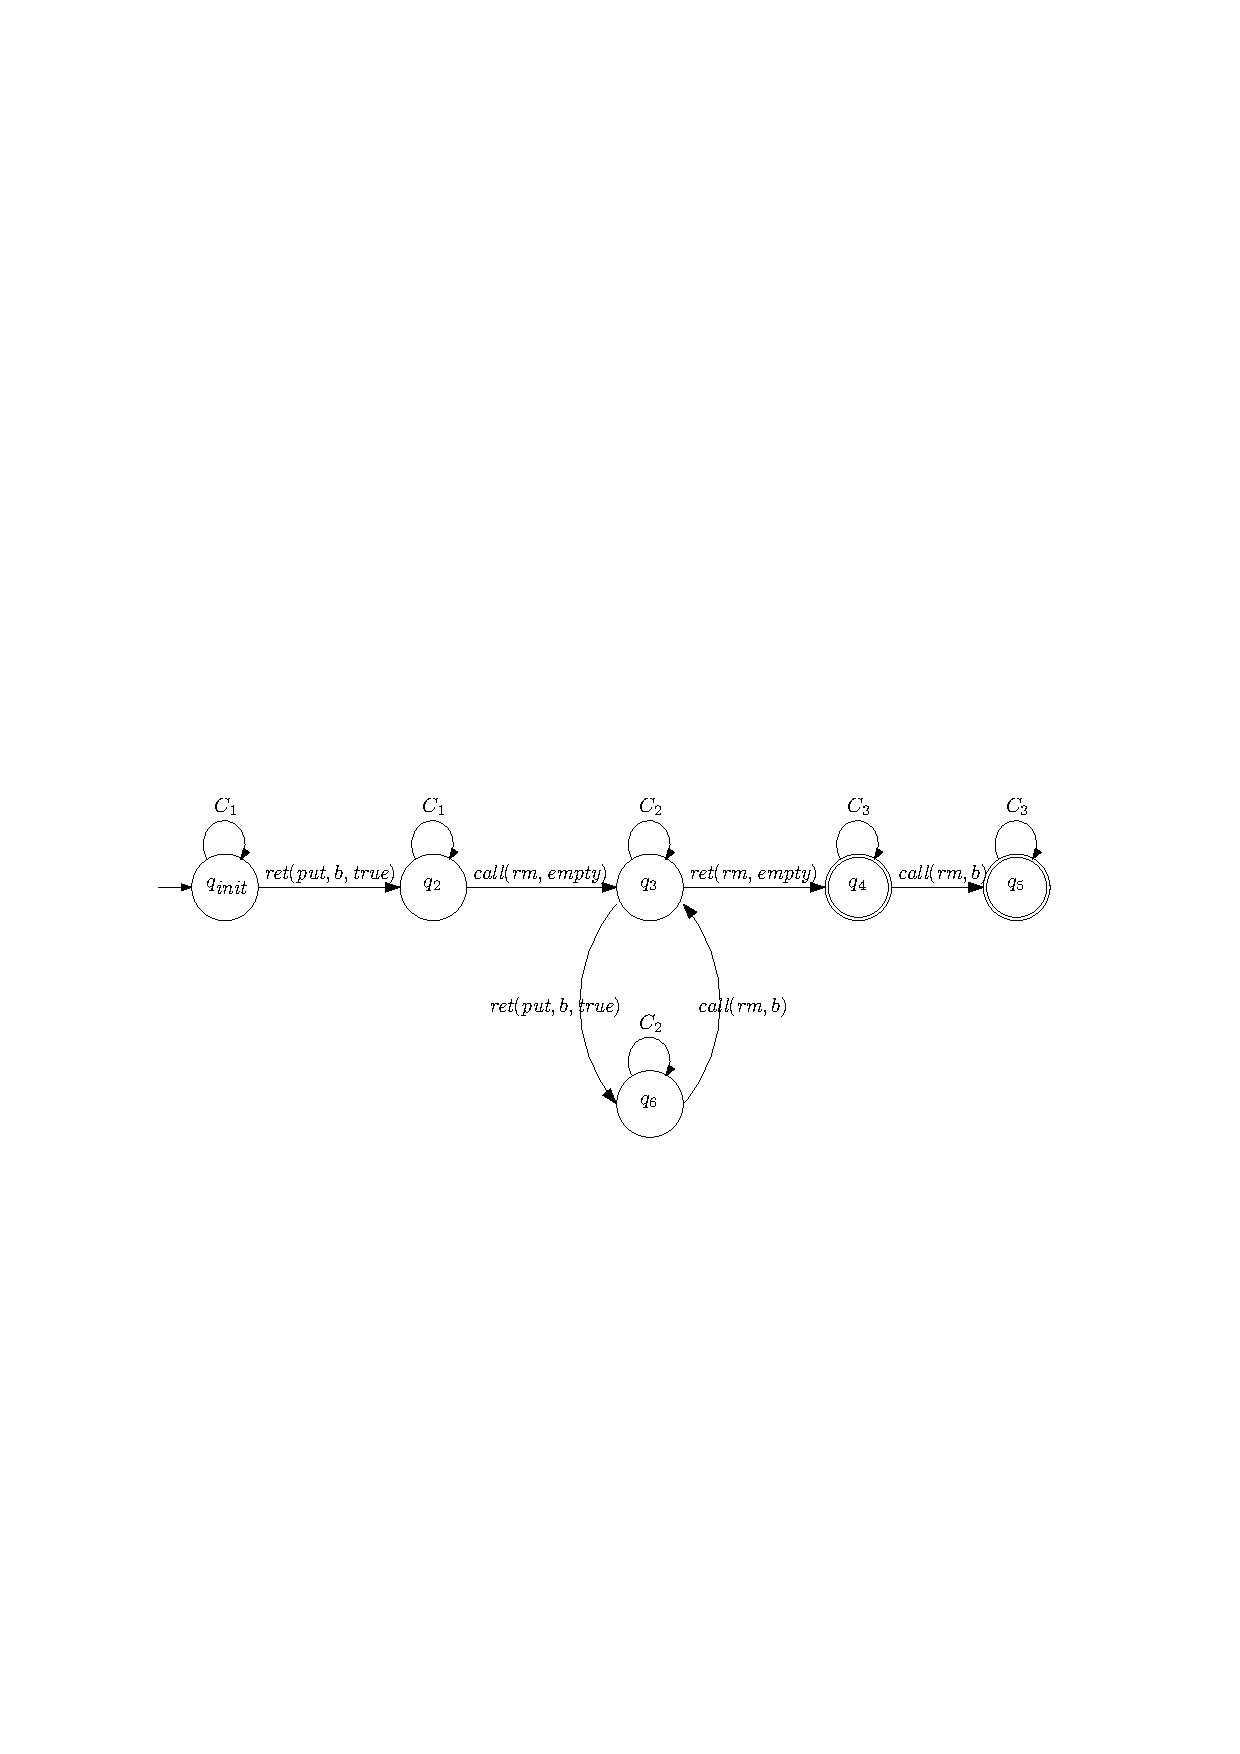
\includegraphics[width=0.8 \textwidth]{figures/PIC_AUTO_PQ3.pdf}
%\vspace{-10pt}
  \caption{Automaton $\mathcal{A}_{\seqPQ}^3$}
  \label{fig:automata for PQ3}
\end{figure}

Given a data-differentiated execution $e$, we say that $o = \textit{rm}(\textit{empty})$ in $e$ is covered by items $d_1,\ldots,d_m$ in $h$, if

\begin{itemize}
\setlength{\itemsep}{0.5pt}
\item[-] $\textit{put}(d_m,\_)$ happens before $o$,

\item[-] For each $i < 1 \leq m$,$\textit{put}(d_{\textit{i-1}},\_)$ happens before $\textit{rm}(d_i)$,

\item[-] $o$ happens before $\textit{rm}(d_1)$, or $\textit{rm}(d_1)$ does not exists in $e$
\end{itemize}

According to the definition of left-right constraint for $o$, in a data-differentiated execution $e$, there is a cycle going through $o$, if and only if there exists items $d_1,\ldots,d_m$, such that $o$ is covered by $d_1,\ldots,d_m$.


\begin{restatable}{lemma}{EPQ3IsCoRegular}
\label{lemma:EPQ3 is co-regular}
$\seqPQ_3$ is co-regular.
\end{restatable}

\begin {proof}

We need to prove that, given a data-independence implementation $\mathcal{I}$, $\mathcal{A}_{\seqPQ}^3 \cap \mathcal{I} \neq \emptyset$ if and only if $\exists e \in \mathcal{I}_{\neq},e' \in \textit{proj}(e), last(e')=\seqPQ_3 \wedge e$ does not linearizable w.r.t. $\textit{MS}(\seqPQ_3)$.

By Lemma \ref{lemma:Lin Equals Constraint for EPQ3}, we need to prove the following fact:

\noindent {\bf $\textit{fact}_1$}: Given a data-independence implementation $\mathcal{I}$, $\mathcal{A}_{\seqPQ}^3 \cap \mathcal{I} \neq \emptyset$ if and only if $\exists e \in \mathcal{I}_{\neq},e' \in \textit{proj}(e), last(e')=\seqPQ_3$, $o = \textit{rm}(\textit{empty})$ is in $e'$, and $o$ is covered by some items $d_1,\ldots,d_m$ in $e'$.


\noindent The $\textit{only if}$ direction: Assume that $e_1 \in \mathcal{I}$ is accepted by $\mathcal{A}_{\seqPQ}^3$. By data-independence, there exists data-differentiated execution $e_2 \in \mathcal{I}$ and a renaming function $r$, such that $e_1=r(e_2)$. Let $d_1,\ldots,d_m$ be the items in $e_2$ such that $r(d_i)=b$ for each $1 \leq i \leq m$. Let $e_3 = e_2 \vert_{ \{ o, d_1, \ldots, d_m \} }$. It is obvious that $e_3 \in \textit{proj}(e_2)$ and $\textit{last}(e_3) = \seqPQ_3$. It is easy to see that $o$ is covered by $d_1,\ldots,d_m$.

\noindent The $\textit{if}$ direction: Assume that there exists such $e$, $e'$, $o$ and $d_1,\ldots,d_m$. Then, let $e_1$ be obtained from $e$ by renaming $d_1,\ldots,d_m$ into $b$ and renaming other items into $d$. By data-independence, $e_1 \in \mathcal{I}$. It is easy to see that $e_1$ is accepted by $\mathcal{A}_{\seqPQ}^3$.

This completes the proof of this lemma. \qed
\end {proof}


\forget{
\section{Proofs and Definitions in Section \ref{sec:relate other data structures with extended priority queue}}
\label{sec:appendix proof and definition in section relate other data structures with extended priority queue}


\subsection{Proofs and Definitions in Subsection \ref{subsec:relate multiSet with extended priority queue}}
\label{subsec:appendix proof and definition in section relate multiset with extended priority queue}

In this section, we use the notions of inductive rules, $\textit{last}$ of a sequential execution, step-by-step and co-regular in \cite{Bouajjani:2015}. Since they are quite similar to the corresponding notions of extended priority queues in Section \ref{sec:inductive rules of extended priority queue}, Section \ref{sec:step-by-step linearizability of extended priority queues} and Section \ref{sec:co-regular of extended priority queues}, we do not introduce their definitions here.

Let us first define three predicates:

\begin{itemize}
\setlength{\itemsep}{0.5pt}
\item[-] Given a sequential execution $l$ of multi-set, $\textit{noDE}(l)$ is satisfied when each operation of $l$ is not $\textit{delete}(\textit{empty})$.

\item[-] Given a sequential execution $l$ of multi-set, $\textit{matched-MS}(l)$ is satisfied, if (1) for each item $a \in \mathbb{D}$, if $\textit{insert}(a)$ is in $l$, then $\textit{delete}(a)$ is in $l$, and (2) for each item $a \in \mathbb{D}$, if $\textit{delete}(a)$ is in $l$, then $\textit{insert}(a)$ is in $l$.

\item[-] Given a sequential execution $l$ of multi-set, $l \in \textit{Insert}^*$ is satisfied when each operation of $l$ is a $\textit{insert}$ event.
\end{itemize}

Let $\textit{MSet}$ be the set of sequential executions $w$ which can be derived from the empty word by inductive rules of multi-set. $\textit{MSet}$ is defined by the following inductive rules:

\begin{itemize}
\setlength{\itemsep}{0.5pt}
\item[-] $\textit{MSet}_0 \equiv \epsilon \in \textit{MSet}$.

\item[-] $\textit{MSet}_1 \equiv (u \in \textit{MSet}) \wedge
(u \in \textit{Insert}^*)
\Rightarrow
(u \cdot \textit{insert}(\textit{itm}) \in \textit{MSet})$.

\item[-] $\textit{MSet}_2 \equiv
(u \cdot v \cdot w \in \textit{MSet}) \wedge
(\textit{noDE}(u \cdot v \cdot w))
\Rightarrow
(u \cdot \textit{insert}(\textit{itm}) \cdot v \cdot \textit{delete}(\textit{itm}) \cdot w \in \textit{MSet})$.

\item[-] $\textit{MSet}_3 \equiv
(u \cdot v \in \textit{MSet}) \wedge
(\textit{matched-MS}(u) )
\Rightarrow
(u \cdot \textit{delete}(\textit{empty}) \cdot v \in \textit{MSet})$.
\end{itemize}

Thus, given a sequential execution $e$, we define $\textit{last}(e)$ as the last possible rule to generate $e$ according to the rules of multi-set:

\begin{itemize}
\setlength{\itemsep}{0.5pt}
\item[-] If $e$ contains $\textit{delete}(\textit{empty})$, then $\textit{last}(e) = \textit{MS}_3$.

\item[-] Else, if $e$ contains $\textit{delete}$, then $\textit{last}(e) = \textit{MSet}_2$.

\item[-] Else, if $e$ contains only $\textit{insert}$, then $\textit{last}(e) = \textit{MSet}_1$.

\item[-] Else ($e = \epsilon$), $\textit{last}(e) = \textit{MSet}_0$.
\end{itemize}

The following three lemmas state that the rules for multi-set are step-by-step linearizability.

\begin{restatable}{lemma}{MS1isStepByStepLinearizability}
\label{lemma:MS1 is step-by-step linearizability}
If a differentiated concurrent execution $e$ is linearizable w.r.t. $\textit{MS}(\textit{MSet}_1)$ with witness $x$, then $e \setminus x \sqsubseteq \textit{MSet} \Rightarrow e \sqsubseteq \textit{MSet}$.
\end{restatable}

\begin {proof}
Let $h$ be the data-differentiated history of $e$, and $l$ be an sequential execution such that $h \sqsubseteq l$ and $l$ matches $\textit{MSet}_1$ with witness $x$. Let $h'=h \setminus x$ and assume that $h' \sqsubseteq l' \in \textit{MSet}$. Let $e_{\textit{lp}}$ be an execution with linearization points of $e$ and the linearization points is added according to $l'$. Or we can say, $e_{\textit{lp}}$ is generated from $e$ by instrumenting linearization points, and the projection of $e_{\textit{lp}}$ into operation is $l'$.

Let sequence $e'_{\textit{lp}}$ be generated from $e_{\textit{lp}}$ by adding $\textit{insert}(x)$ at an arbitrary time point between $\textit{call}(\textit{insert},x)$ and $\textit{ret}(\textit{insert},x)$. Let $l''$ be the projection of $e'_{\textit{lp}}$ into operations.

It is easy to see that $h \sqsubseteq l''$. Since $l''$ is obtained from $l'$ by adding one $\textit{insert}(x)$, we can see that $l''$ contains only $\textit{insert}$, and then $l'' \in \textit{MSet}$. \qed
\end {proof}


\begin{restatable}{lemma}{MS2isStepByStepLinearizability}
\label{lemma:MS2 is step-by-step linearizability}
If a differentiated concurrent execution $e$ is linearizable w.r.t. $\textit{MS}(\textit{MSet}_2)$ with witness $x$, then $e \setminus x \sqsubseteq \textit{MSet} \Rightarrow e \sqsubseteq \textit{MSet}$.
\end{restatable}

\begin {proof}
Let $h$ be the data-differentiated history of $e$, and $l$ be an sequential execution such that $h \sqsubseteq l$ and $l$ matches $\textit{MSet}_1$ with witness $x$. Let $h'=h \setminus x$ and assume that $h' \sqsubseteq l' \in \textit{MSet}$. Let $e_{\textit{lp}}$ be an execution with linearization points of $e$ and the linearization points is added according to $l'$. Or we can say, $e_{\textit{lp}}$ is generated from $e$ by instrumenting linearization points, and the projection of $e_{\textit{lp}}$ into operation is $l'$.

It is easy to see that $\textit{delete}(x)$ does not happen before $\textit{insert}(x)$, and then $\textit{call}(\textit{insert},x)$ is before $\textit{ret}(\textit{delete},x)$ in $e$. Let sequence $e'_{\textit{lp}}$ be generated from $e_{\textit{lp}}$ by adding $\textit{insert}(x)$ just after $\textit{call}(\textit{insert},x)$ and adding $\textit{delete}(x)$ just before $\textit{ret}(\textit{delete},x)$. Let $l''$ be the projection of $e'_{\textit{lp}}$ into operations.

It is easy to see that $h \sqsubseteq l''$. Since (1) $l' \in \textit{MSet}$, (2) $l''$ is obtained from $l'$ by adding one $\textit{insert}(x)$ and one $\textit{delete}(x)$, while $\textit{insert}(x)$ is before $\textit{delete}(x)$ (3)and $l'$ does not contain $\textit{delete}(\textit{empty})$, we can see that $l'' \in \textit{MSet}$. \qed
\end {proof}


\begin{restatable}{lemma}{MS3isStepByStepLinearizability}
\label{lemma:MS3 is step-by-step linearizability}
If a differentiated concurrent execution $e$ is linearizable w.r.t. $\textit{MS}(\textit{MSet}_3)$ and $o$ is a $\textit{delete}(\textit{empty})$ event, then $e \setminus o \sqsubseteq \textit{MSet} \Rightarrow e \sqsubseteq \textit{MSet}$.
\end{restatable}

\begin {proof}
This Lemma can be similarly proved as Lemma \ref{lemma:EPQ3 is step-by-step linearizability}. \qed
\end {proof}

The following lemma states that $\textit{MSet}_1$ is always co-regular.

\begin{restatable}{lemma}{MS1IsAlwaysCoRegular}
\label{lemma:MS1 is always co-regular}
Given a differentiated execution $e$, if $\textit{last}(e) = \textit{MSet}_1$, then $e \sqsubseteq \textit{MS}(\textit{MSet}_1)$.
\end{restatable}

\begin {proof}
Since $\textit{last}(e) = \textit{MSet}_1$, there are only $\textit{insert}$ in $e$. Then no matter how we locate linearization points of operations of $e$, we can always obtain a sequence in $\textit{MS}(\textit{MSet}_1)$. This completes the proof of this lemma. \qed
\end {proof}

The following lemma shows how to detect violation to $\textit{MS}(\textit{MSet}_2)$.

\begin{restatable}{lemma}{ReduceMS2intoOneValue}
\label{lemma:reduce MS2 into one value}
Given a differentiated execution $e$, there exists some $e' \in \textit{proj}(e)$, such that $\textit{last}(e') = \textit{MSet}_2$ and $e'$ doe not linearizable w.r.t $\textit{MS}(\textit{MSet}_2)$, if and only if one of the following case holds for some $x \in \mathbb{D}$.
\begin{itemize}
\setlength{\itemsep}{0.5pt}
\item[-] $\textit{delete}(x)$ is in $e$ while $\textit{insert}(x)$ is not in $e$.

\item[-] there is more than one $\textit{delete}(x)$ in $e$ and one $\textit{insert}(x)$ in $e$.

\item[-] $\textit{delete}(x) <_{\textit{hb}} \textit{insert}(x)$ in $e$.
\end{itemize}
\end{restatable}

\begin {proof}

The $\textit{only if}$ is obvious and omitted here.

To prove the $\textit{if}$ direction, we prove its contrapositive. Assume that for each item $x$ of $e$, the following conditions are satisfied:

\begin{itemize}
\setlength{\itemsep}{0.5pt}
\item[-] If $\textit{delete}(x)$ is in $e$, then $\textit{insert}(x)$ is also in $e$.

\item[-] There is at most $\textit{delete}(x)$ in $e$.

\item[-] $\textit{delete}(x)$ does not happen before $\textit{insert}(x)$.
\end{itemize}

Assume by contradiction that there exists some $e' \in \textit{proj}(e)$, such that $\textit{last}(e') = \textit{MSet}_2$ and $e'$ doe not linearizable w.r.t $\textit{MS}(\textit{MSet}_2)$. Since $\textit{last}(e') = \textit{MSet}_2$, there exists $\textit{delete}$ in $e$. Let this $\textit{delete}$ operation be $\textit{delete}(a)$. By assumption, we know that in $e$ there exists one $\textit{insert}(a)$ and one $\textit{delete}(a)$, and $\textit{delete}(a)$ does not happen before $\textit{insert}(a)$. Then we know that $\textit{call}(\textit{insert},x)$ is before $\textit{ret}(\textit{delete},x)$.

Let $e_{\textit{lp}}$ be generated from $e$ by (1) put the linearization of $\textit{insert}(x)$ just after $\textit{call}(\textit{insert},x)$, (2) put the linearization of $\textit{delete}(x)$ just before $\textit{ret}(\textit{insert},x)$, and (3) for other operations, put its linearization point at an arbitrary between its call and return actions. Let $l'$ be the projection of $e_{\textit{lp}}$ into operations. It is obvious that $h \sqsubseteq l'$. According to our construction of $e_{\textit{lp}}$, we can see that in $l'$, $\textit{insert}(x)$ is before $\textit{delete}(x)$. Therefore, we can see that $l' \in \textit{MS}(\textit{MSet}_2)$, which contradicts our assumption. This completes the proof of the $\textit{id}$ direction. \qed
\end {proof}

According to Lemma \ref{lemma:reduce MS2 into one value}, to check violation to $\textit{MS}(\textit{MSet}_2)$, we need to consider three cases for some $b \in \mathbb{D}$: (1) there is $\textit{delete}(b)$ but there is not $\textit{insert}(x)$, (2) there is more than one $\textit{delete}(b)$ and one $\textit{insert}(b)$ in $e$, and (3) $\textit{delete}(b) <_{\textit{hb}} \textit{insert}(b)$.

For each such case, we construct a register automata. We generate register automata $\mathcal{A}_{\textit{MS}}^1$ for the first case, and it is shown in \figurename~\ref{fig:automata 1 for MS-2 in appendix}. Here $c_1 = \textit{call}(\textit{insert},a),\textit{ret}(\textit{insert},a)$, $\textit{call}(\textit{delete},a),\textit{ret}(\textit{delete},a),
\textit{call}(\textit{delete},\textit{empty}),\textit{ret}(\textit{delete},\textit{empty})$, $c_2 = c_1 + \textit{call}(\textit{delete},b) + \textit{ret}(\textit{delete},b)$.


\begin{figure}[htbp]
  \centering
  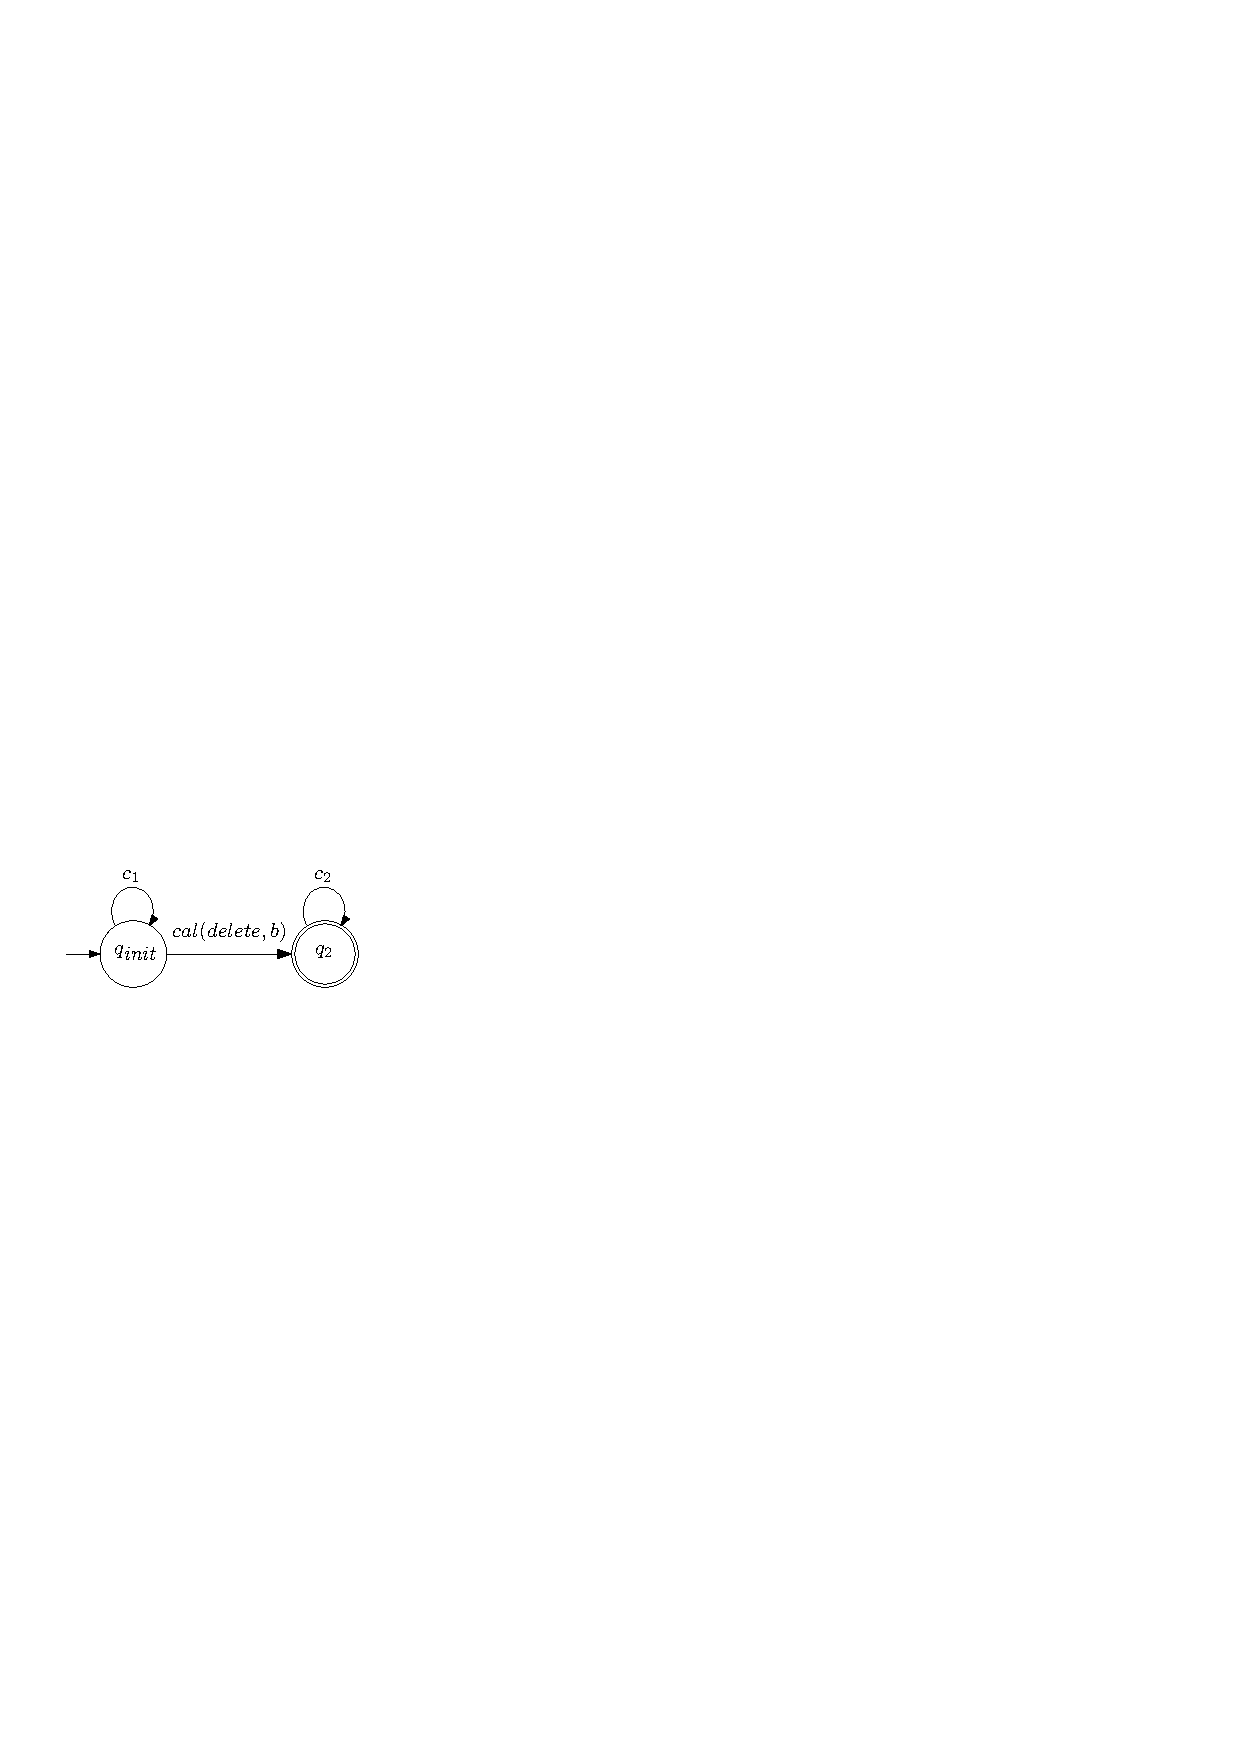
\includegraphics[width=0.3 \textwidth]{figures/PIC_AUTO_MS_1.pdf}
%\vspace{-10pt}
  \caption{Automaton $\mathcal{A}_{\textit{MS}}^1$}
  \label{fig:automata 1 for MS-2 in appendix}
\end{figure}


We generate register automata $\mathcal{A}_{\textit{MS}}^2$ for the second case, and it is shown in \figurename~\ref{fig:automata 2 for MS-2 in appendix}. Here $c_1 = \textit{call}(\textit{insert},a),\textit{ret}(\textit{insert},a), \textit{call}(\textit{delete},a),\textit{ret}(\textit{delete},a),\textit{call}(\textit{delete},\textit{empty})$, $\textit{ret}(\textit{delete},\textit{empty})$, $c_2 = c_1 + \textit{ret}(\textit{insert},b)$, $c_3 = c_2 + \textit{ret}(\textit{delete},b)$, $c_4 = c_3 + \textit{call}(\textit{delete},b)$, $c_5 = c_1 + \textit{ret}(\textit{delete},b)$, $c_6 = c_5 + \textit{call}(\textit{delete},b)$.

\begin{figure}[htbp]
  \centering
  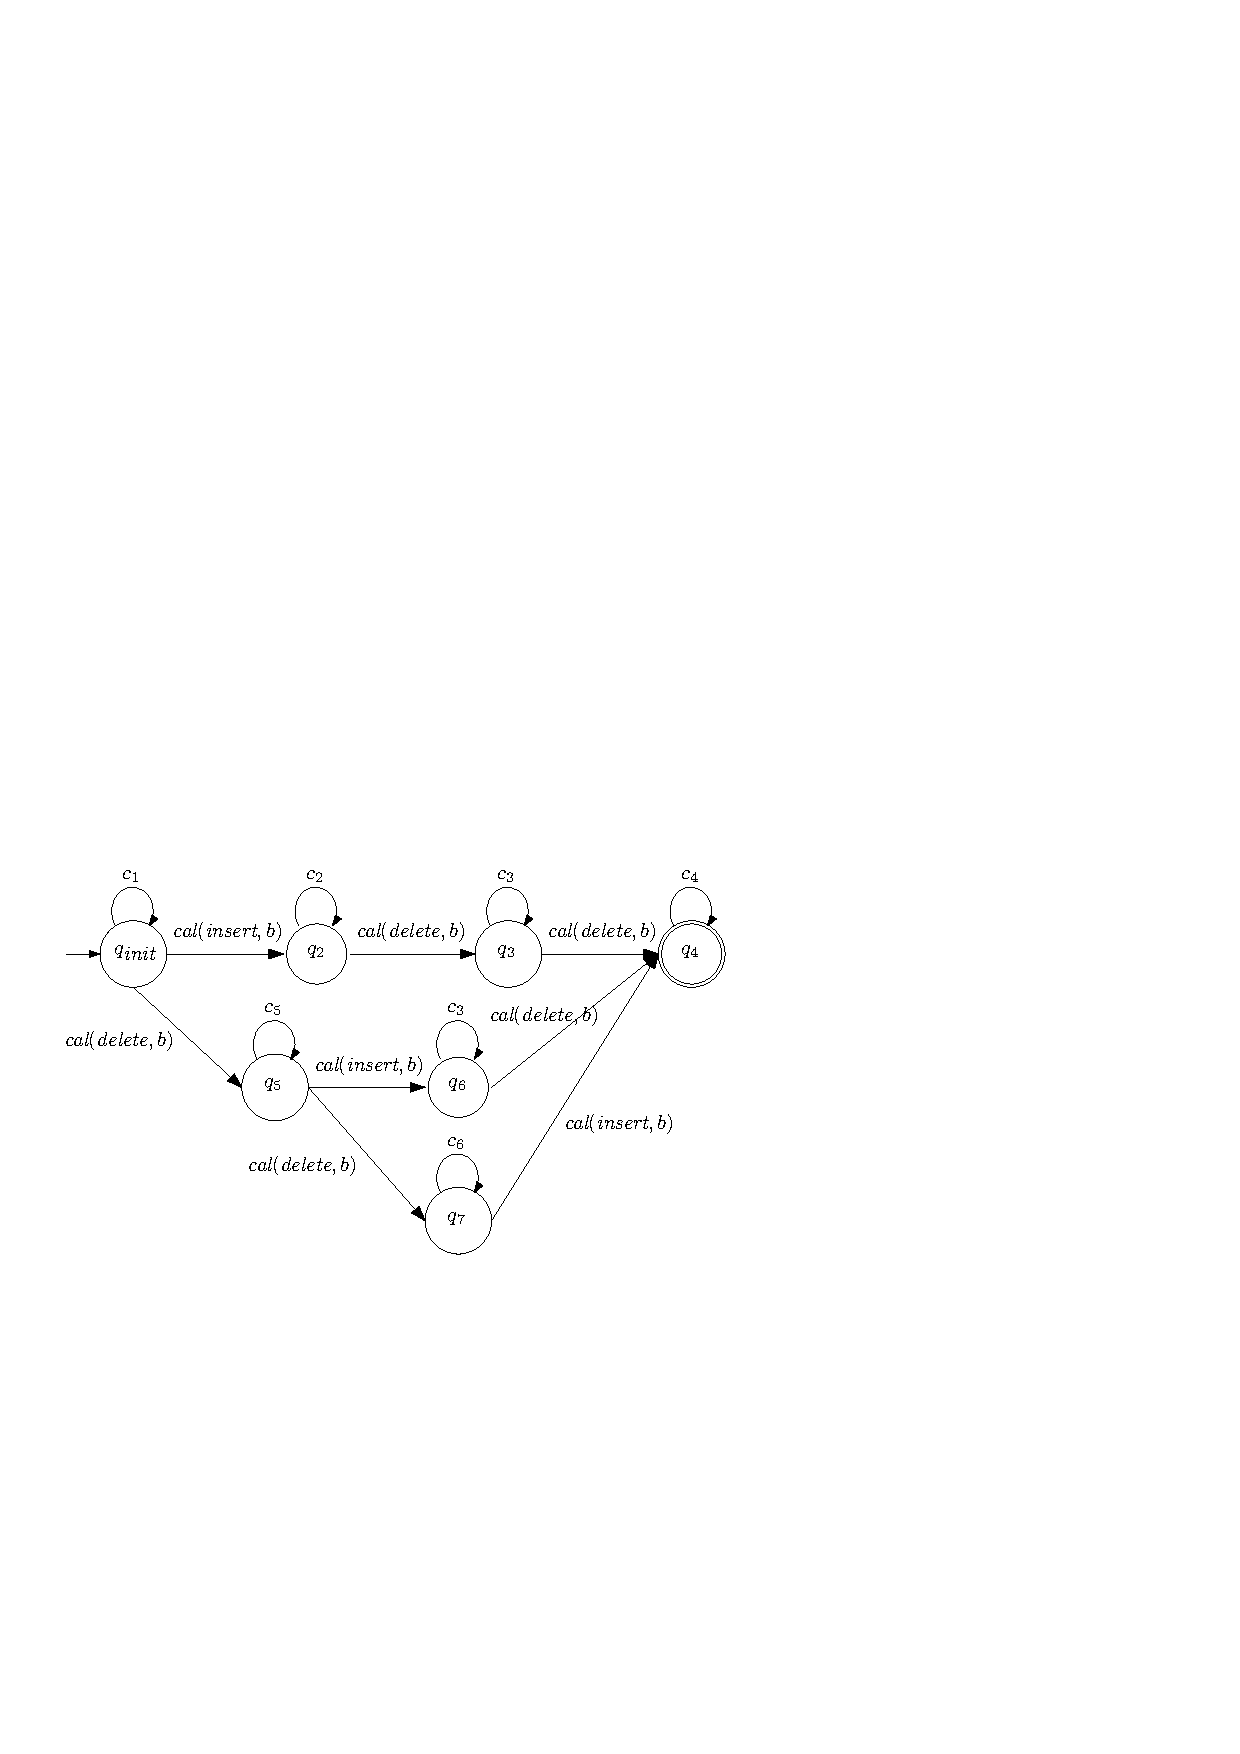
\includegraphics[width=0.7 \textwidth]{figures/PIC_AUTO_MS_2.pdf}
%\vspace{-10pt}
  \caption{Automaton $\mathcal{A}_{\textit{MS}}^2$}
  \label{fig:automata 2 for MS-2 in appendix}
\end{figure}


We generate register automata $\mathcal{A}_{\textit{MS}}^3$ for the third case, and it is shown in \figurename~\ref{fig:automata 3 for MS-2 in appendix}. Here $c_1 = \textit{call}(\textit{insert},a)$, $\textit{ret}(\textit{insert},a)$, $\textit{call}(\textit{delete},a)$, $\textit{ret}(\textit{delete},a),\textit{call}(\textit{delete},b)$, $\textit{call}($ $\textit{delete},\textit{empty}),\textit{ret}(\textit{delete},\textit{empty})$, $c_2 = c_1 + \textit{ret}(\textit{delete},b)$, $c_3 = c_2 + \textit{ret}(\textit{insert},b)$.

\begin{figure}[htbp]
  \centering
  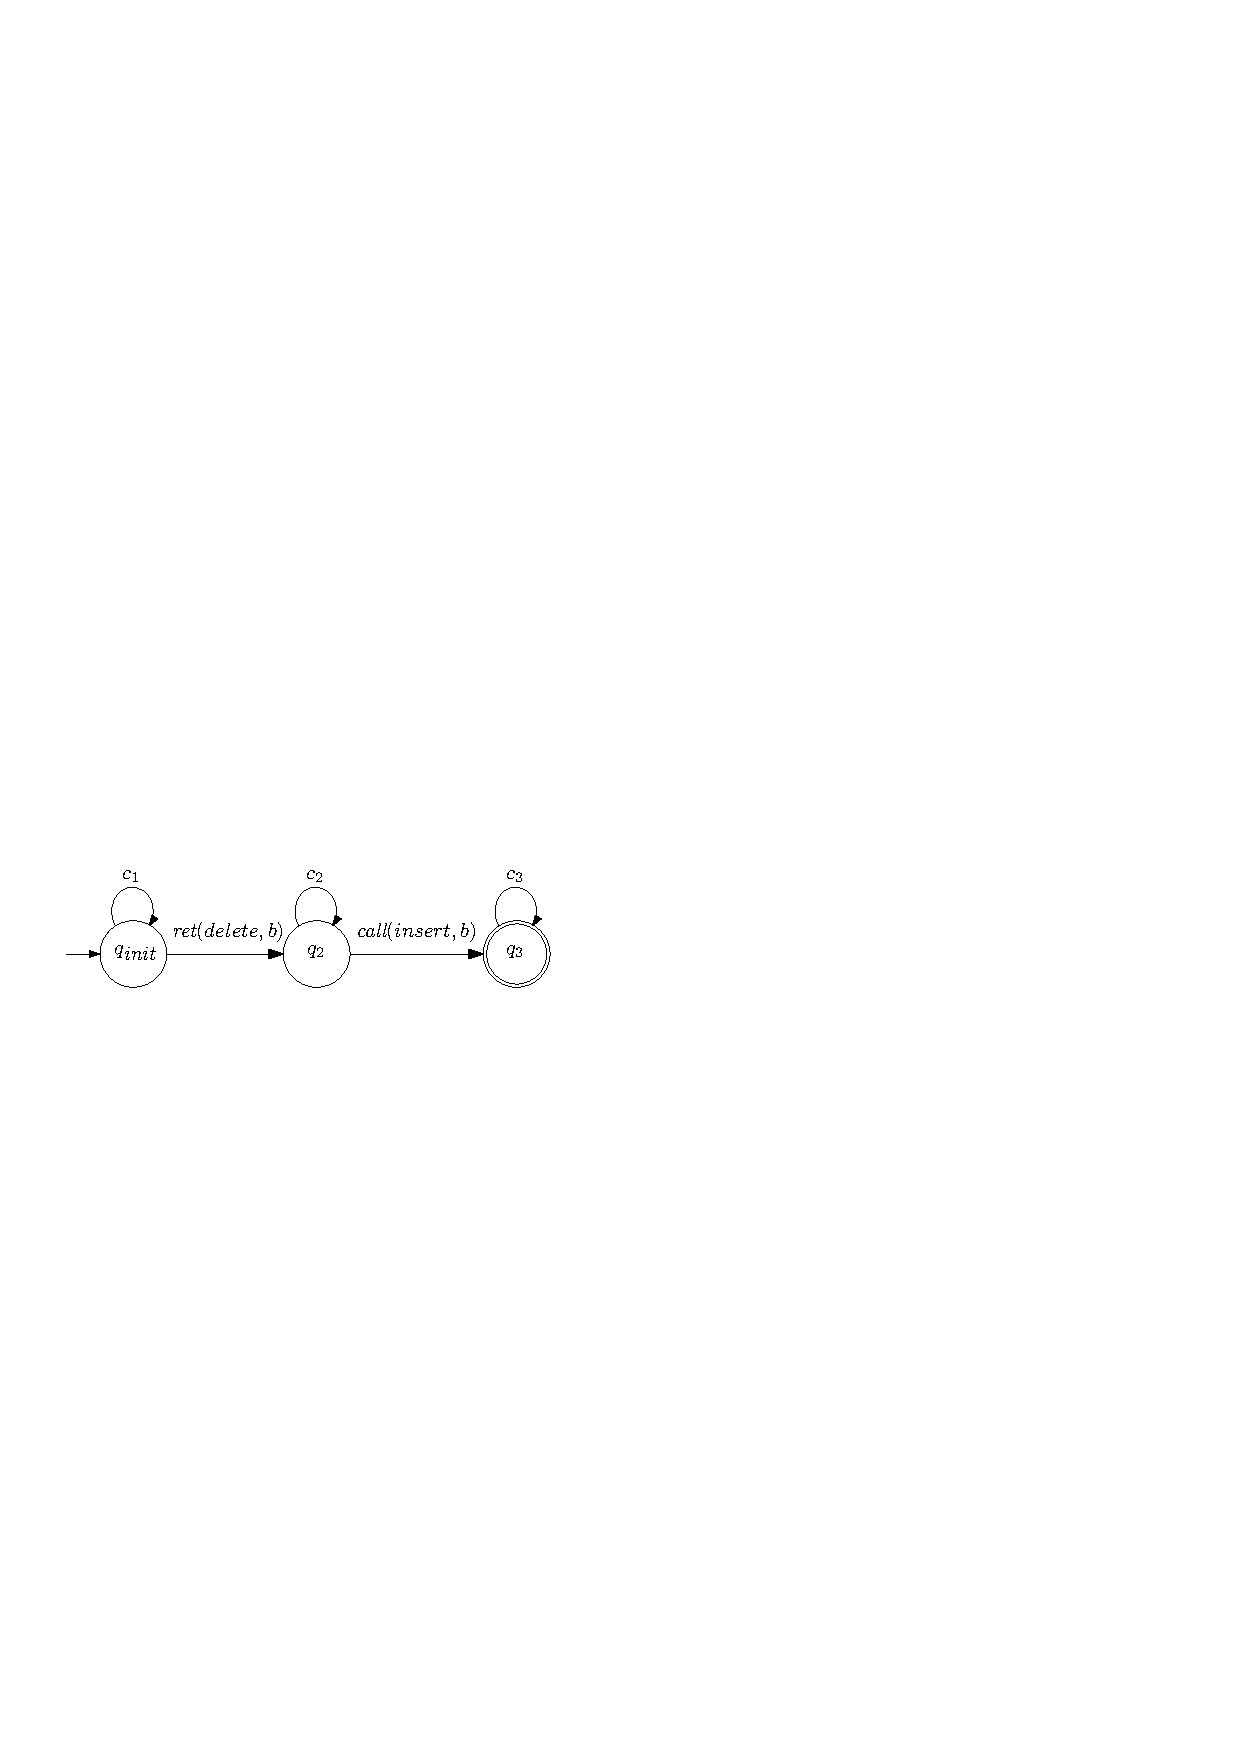
\includegraphics[width=0.6 \textwidth]{figures/PIC_AUTO_MS_3.pdf}
%\vspace{-10pt}
  \caption{Automaton $\mathcal{A}_{\textit{MS}}^3$}
  \label{fig:automata 3 for MS-2 in appendix}
\end{figure}


Let $\textit{Auts}_{\textit{2-ms}} = \{ \mathcal{A}_{\textit{MS}}^1, \mathcal{A}_{\textit{MS}}^2, \mathcal{A}_{\textit{MS}}^3 \}$. The following lemma states that $\textit{MS}_2$ is co-regular.


\begin{restatable}{lemma}{MS2IsCoRegular}
\label{lemma:MS2 is co-regular}
$\textit{MSet}_2$ is co-regular.
\end{restatable}

\begin {proof}

According to \cite{Bouajjani:2015}, we need to prove that, given a independence implementation $\mathcal{I}$, $\textit{Auts}_{\textit{2-ms}} \cap \mathcal{I} \neq \emptyset$, if and only if $\exists e \in \mathcal{I}_{\neq},$ $e' \in \textit{proj}(e),$ $\textit{last}(e') = \textit{MSet}_2 \wedge e'$ does not linearizable w.r.t. $\textit{MS}(\textit{MSet}_2)$.

By Lemma \ref{lemma:reduce MS2 into one value}, we need to prove the following fact:

\noindent {\bf $\textit{fact}_1$}: given a independence implementation $\mathcal{I}$, $\textit{Auts}_{\textit{2-ms}} \cap \mathcal{I} \neq \emptyset$, if and only if $\exists e \in \mathcal{I}_{\neq}$, and one of the following case holds for some $x \in \mathbb{D}$.
\begin{itemize}
\setlength{\itemsep}{0.5pt}
\item[-] $\textit{delete}(x)$ is in $e$ while $\textit{insert}(x)$ is not in $e$.

\item[-] there is more than one $\textit{delete}(x)$ in $e$ and one $\textit{insert}(x)$ in $e$.

\item[-] $\textit{delete}(x) <_{\textit{hb}} \textit{insert}(x)$ in $e$.
\end{itemize}

\noindent The $\textit{only if}$ direction: Assume that $e_1 \in \mathcal{I}$ is accepted by some register automata in $\textit{Auts}_{\textit{1-eq}}$. By data-independence, there exists data-differentiated execution $e_2 \in \mathcal{I}$ and a renaming function $r$, such that $e_1=r(e_2)$. Since $e_1$ is accepted by some register automata in  $\textit{Auts}_{\textit{1-eq}}$, let $y$ be the item that are renamed into $b$ by $r$. Then it is not hard to see that $y$ satisfies one of three conditions in $e_2$.

\noindent The $\textit{if}$ direction: Assume that there exists such $e \in \mathcal{I}_{\neq}$ and $x$. Let renaming function $r$ maps $x$ into $b$ and all other items into $a$. By data-independence, we can see that $r(e) \in \mathcal{I}$. Then it is easy to see that $r(e)$ is accepted by some automaton in $\textit{Auts}_{\textit{2-ms}}$. \qed
\end {proof}

Similar to Lemma \ref{lemma:EPQ3 is co-regular}, we can prove that $\textit{MSet}_3$ is co-regular, as stated by the following lemma.

\begin{restatable}{lemma}{MSet3IsCoRegular}
\label{lemma:MSet3 is co-regular}
$\textit{MSet}_3$ is co-regular.
\end{restatable}

Similar as register automata for $\seqPQ_3$, we have register automata $\mathcal{A}_{\textit{MS}}^4$ for $\textit{MSet}_3$, which is shown in \figurename~\ref{fig:automata 4 for MS-3 in appendix}. In \figurename~\ref{fig:automata 4 for MS-3 in appendix}, let $c = \textit{call}(\textit{insert},d),\textit{ret}(\textit{insert},d), \textit{call}(\textit{delete},d)$, $\textit{ret}(\textit{delete},d),\textit{call}(\textit{delete},\textit{empty}),\textit{ret}(\textit{delete},\textit{empty})$, $c_1 = c + \textit{call}(\textit{insert},b)$, $c_2 = c_1 + \textit{ret}(\textit{delete},b)$, and $c_3 = c + \textit{ret}(\textit{delete},b)$.

\begin{figure}[htbp]
  \centering
  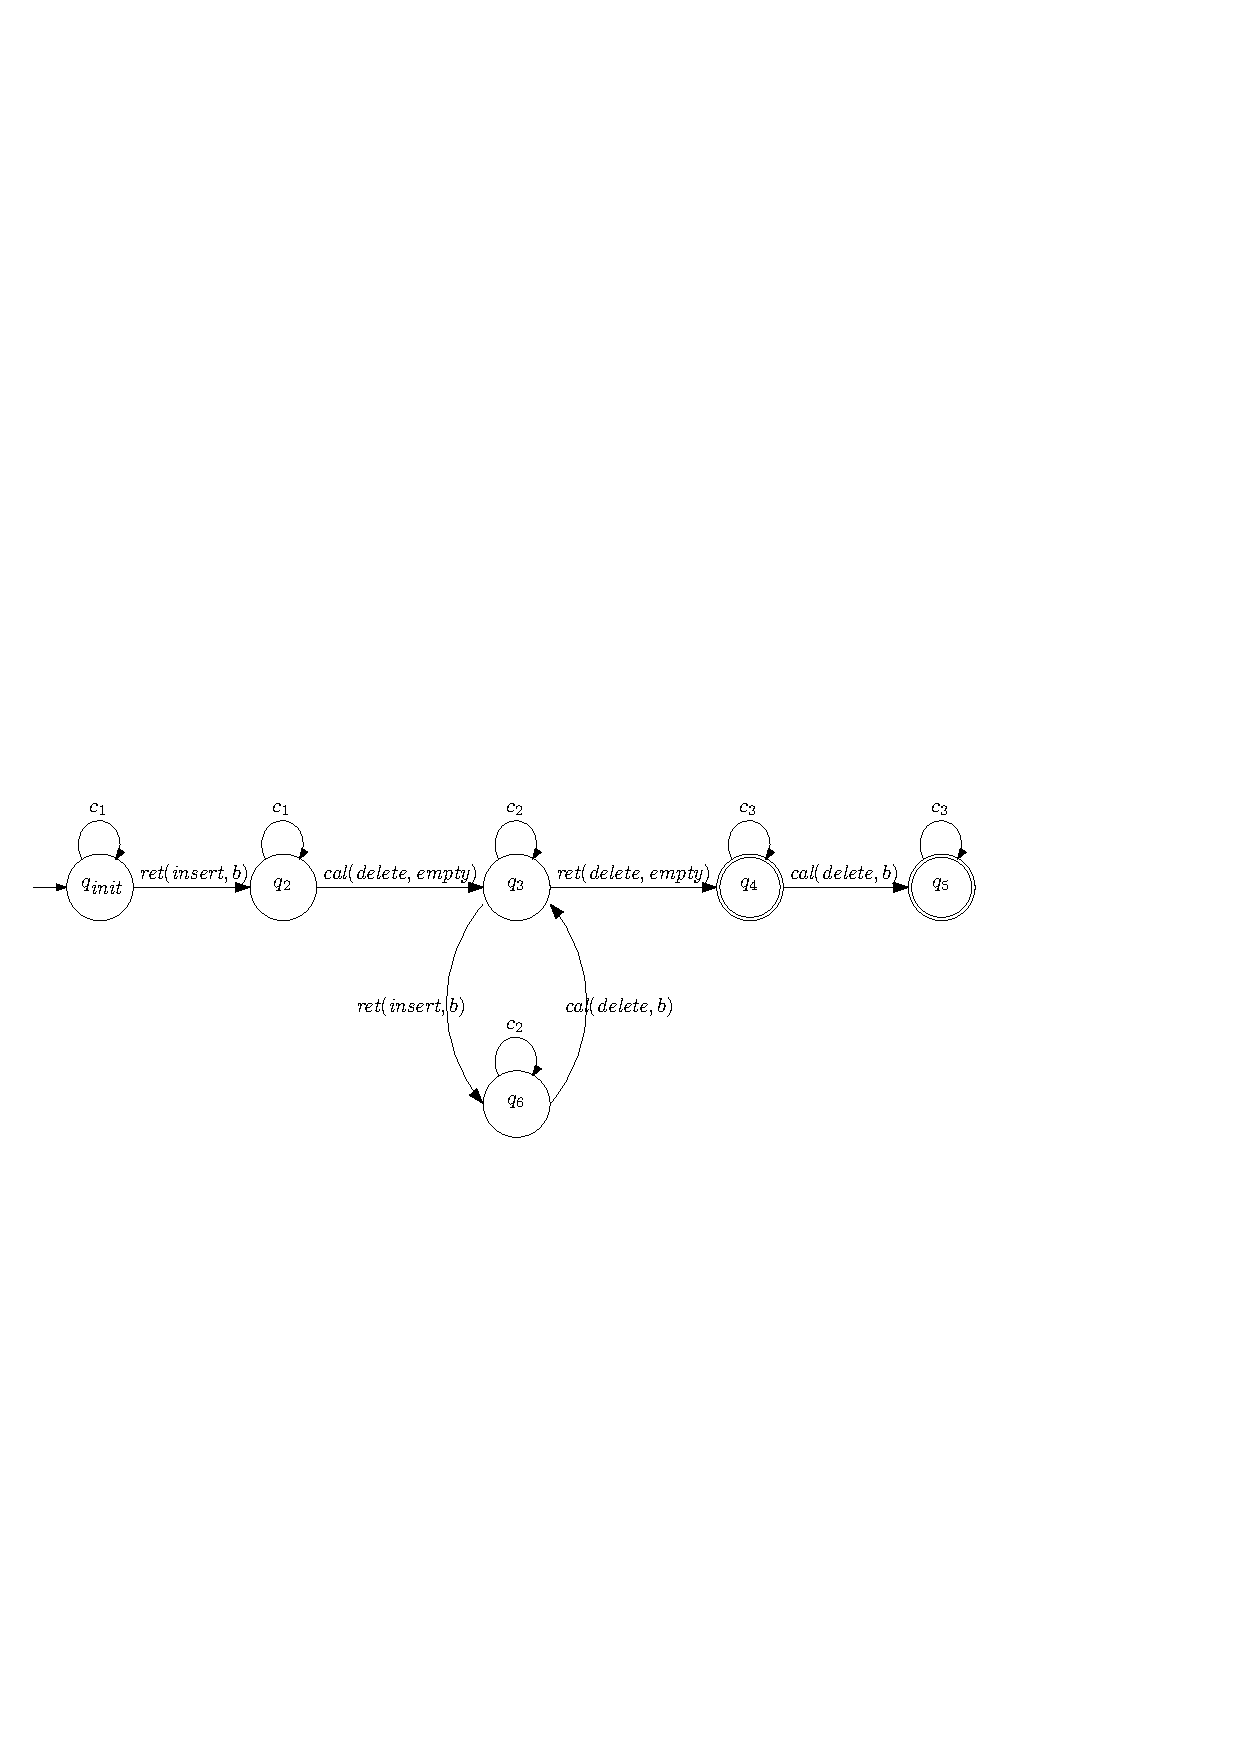
\includegraphics[width=0.8 \textwidth]{figures/PIC_AUTO_MS_4.pdf}
%\vspace{-10pt}
  \caption{Automaton $\mathcal{A}_{\textit{MS}}^4$}
  \label{fig:automata 4 for MS-3 in appendix}
\end{figure}

The following lemma shows that our transformation from multi-set into extended priority queue is correct.

\RelateMultiSetwithEPQ*

\begin {proof}

For the $\textit{only if}$ direction, given an execution $e_m \in \mathcal{I}_m$ of multi-set, such that $e_m$ is accepted by some automaton in $\textit{Auts}_{\textit{MS}}$. If $e_m$ is accepted by $\mathcal{A}_{\textit{MS}}^1$, $\mathcal{A}_{\textit{MS}}^2$, $\mathcal{A}_{\textit{MS}}^3$ or $\mathcal{A}_{\textit{MS}}^4$, then it is easy to see that $\textit{MStoEPQ}(e_m)$ is accepted by $\mathcal{A}_{\textit{SinPri}}^2$, $\mathcal{A}_{\textit{SinPri}}^3$, $\mathcal{A}_{\textit{SinPri}}^1$ or $\mathcal{A}_{\seqPQ}^3$, respectively.

For the $\textit{if}$ direction, given an execution $e_{\textit{epq}}$ of extended priority queue, such that $e_{\textit{epq}} = \textit{MStoEPQ}(e_m)$ for some $e_m$ of multi-set, and $e_{\textit{epq}}$ is accepted by some automaton in $\textit{Auts}_{\seqPQ}$.

According to definition of $\textit{MStoEPQ}$, we can see that (1) in $e_{\textit{epq}}$ there does not exist two items with comparable priorities, and (2) in $e_{\textit{epq}}$, there does not exists two items with a same priority. Therefore, the register automata for $\seqPQ_1$ and the register automaton $\mathcal{A}_{\textit{SinPri}}^4$ can be safely ignored. Then, if $e_{\textit{epq}}$ is accepted by $\mathcal{A}_{\textit{SinPri}}^1$, $\mathcal{A}_{\textit{SinPri}}^2$, $\mathcal{A}_{\textit{SinPri}}^3$ or $\mathcal{A}_{\seqPQ}^3$, then it is easy to see that $e_m$ is accepted by $\mathcal{A}_{\textit{MS}}^3$, $\mathcal{A}_{\textit{MS}}^1$, $\mathcal{A}_{\textit{MS}}^2$ and $\mathcal{A}_{\textit{MS}}^4$, respectively. \qed
\end {proof}



\subsection{Proofs and Definitions in Subsection \ref{subsec:relate stack with extended priority queue}}
\label{subsec:appendix proof and definition in section relate stack with extended priority queue}
}





